%% (Master) Thesis template
% Template version used: v1.4
%
% Largely adapted from Adrian Nievergelt's template for the ADPS
% (lecture notes) project.


%% We use the memoir class because it offers a many easy to use features.
\documentclass[11pt,a4paper,titlepage]{memoir}

%% Packages
%% ========

%% LaTeX Font encoding -- DO NOT CHANGE
\usepackage[OT1]{fontenc}

%% Babel provides support for languages.  'english' uses British
%% English hyphenation and text snippets like "Figure" and
%% "Theorem". Use the option 'ngerman' if your document is in German.
%% Use 'american' for American English.  Note that if you change this,
%% the next LaTeX run may show spurious errors.  Simply run it again.
%% If they persist, remove the .aux file and try again.
\usepackage[english]{babel}

%% Input encoding 'utf8'. In some cases you might need 'utf8x' for
%% extra symbols. Not all editors, especially on Windows, are UTF-8
%% capable, so you may want to use 'latin1' instead.
\usepackage[utf8]{inputenc}

%% This changes default fonts for both text and math mode to use Herman Zapfs
%% excellent Palatino font.  Do not change this.
\usepackage[sc]{mathpazo}

%% The AMS-LaTeX extensions for mathematical typesetting.  Do not
%% remove.
\usepackage{amsmath,amssymb,amsfonts,mathrsfs}

%% NTheorem is a reimplementation of the AMS Theorem package. This
%% will allow us to typeset theorems like examples, proofs and
%% similar.  Do not remove.
%% NOTE: Must be loaded AFTER amsmath, or the \qed placement will
%% break
\usepackage[amsmath,thmmarks]{ntheorem}

%% LaTeX' own graphics handling
\usepackage{graphicx}

%% We unfortunately need this for the Rules chapter.  Remove it
%% afterwards; or at least NEVER use its underlining features.
\usepackage{soul}

%% This allows you to add .pdf files. It is used to add the
%% declaration of originality.
\usepackage{pdfpages}

%% Some more packages that you may want to use.  Have a look at the
%% file, and consult the package docs for each.
%% See the TeXed file for more explanations

%% [OPT] Multi-rowed cells in tabulars
%\usepackage{multirow}

%% [REC] Intelligent cross reference package. This allows for nice
%% combined references that include the reference and a hint to where
%% to look for it.
\usepackage{varioref}

%% [OPT] Easily changeable quotes with \enquote{Text}
%\usepackage[german=swiss]{csquotes}

%% [REC] Format dates and time depending on locale
\usepackage{datetime}

%% [OPT] Provides a \cancel{} command to stroke through mathematics.
%\usepackage{cancel}

%% [NEED] This allows for additional typesetting tools in mathmode.
%% See its excellent documentation.
\usepackage{mathtools}

%% [ADV] Conditional commands
%\usepackage{ifthen}

%% [OPT] Manual large braces or other delimiters.
%\usepackage{bigdelim, bigstrut}

%% [REC] Alternate vector arrows. Use the command \vv{} to get scaled
%% vector arrows.
\usepackage[h]{esvect}

%% [NEED] Some extensions to tabulars and array environments.
\usepackage{array}

%% [OPT] Postscript support via pstricks graphics package. Very
%% diverse applications.
%\usepackage{pstricks,pst-all}

%% [?] This seems to allow us to define some additional counters.
%\usepackage{etex}

%% [ADV] XY-Pic to typeset some matrix-style graphics
%\usepackage[all]{xy}

%% [OPT] This is needed to generate an index at the end of the
%% document.
%\usepackage{makeidx}

%% [OPT] Fancy package for source code listings.  The template text
%% needs it for some LaTeX snippets; remove/adapt the \lstset when you
%% remove the template content.
\usepackage{listings}
\lstset{language=TeX,basicstyle={\normalfont\ttfamily}}

%% [REC] Fancy character protrusion.  Must be loaded after all fonts.
\usepackage{microtype}

%% [REC] Nicer tables.  Read the excellent documentation.
\usepackage{booktabs}

%% My additional packages
\usepackage{tikz}
\usepackage{float}
\usepackage{subcaption}


%% Our layout configuration.  DO NOT CHANGE.
%% Memoir layout setup

%% NOTE: You are strongly advised not to change any of them unless you
%% know what you are doing.  These settings strongly interact in the
%% final look of the document.

% Dependencies
\usepackage{template/ETHlogo}

% Turn extra space before chapter headings off.
\setlength{\beforechapskip}{0pt}

\nonzeroparskip
\parindent=0pt
\defaultlists

% Chapter style redefinition
\makeatletter

\if@twoside
  \pagestyle{Ruled}
  \copypagestyle{chapter}{Ruled}
\else
  \pagestyle{ruled}
  \copypagestyle{chapter}{ruled}
\fi
\makeoddhead{chapter}{}{}{}
\makeevenhead{chapter}{}{}{}
\makeheadrule{chapter}{\textwidth}{0pt}
\copypagestyle{abstract}{empty}

\makechapterstyle{bianchimod}{%
  \chapterstyle{default}
  \renewcommand*{\chapnamefont}{\normalfont\Large\sffamily}
  \renewcommand*{\chapnumfont}{\normalfont\Large\sffamily}
  \renewcommand*{\printchaptername}{%
    \chapnamefont\centering\@chapapp}
  \renewcommand*{\printchapternum}{\chapnumfont {\thechapter}}
  \renewcommand*{\chaptitlefont}{\normalfont\huge\sffamily}
  \renewcommand*{\printchaptertitle}[1]{%
    \hrule\vskip\onelineskip \centering \chaptitlefont\textbf{\vphantom{gyM}##1}\par}
  \renewcommand*{\afterchaptertitle}{\vskip\onelineskip \hrule\vskip
    \afterchapskip}
  \renewcommand*{\printchapternonum}{%
    \vphantom{\chapnumfont {9}}\afterchapternum}}

% Use the newly defined style
\chapterstyle{bianchimod}

\setsecheadstyle{\Large\bfseries\sffamily}
\setsubsecheadstyle{\large\bfseries\sffamily}
\setsubsubsecheadstyle{\bfseries\sffamily}
\setparaheadstyle{\normalsize\bfseries\sffamily}
\setsubparaheadstyle{\normalsize\itshape\sffamily}
\setsubparaindent{0pt}

% Set captions to a more separated style for clearness
\captionnamefont{\sffamily\bfseries\footnotesize}
\captiontitlefont{\sffamily\footnotesize}
\setlength{\intextsep}{16pt}
\setlength{\belowcaptionskip}{1pt}

% Set section and TOC numbering depth to subsection
\setsecnumdepth{subsection}
\settocdepth{subsection}

%% Titlepage adjustments
\pretitle{\vspace{0pt plus 0.7fill}\begin{center}\HUGE\sffamily\bfseries}
\posttitle{\end{center}\par}
\preauthor{\par\begin{center}\let\and\\\Large\sffamily}
\postauthor{\end{center}}
\predate{\par\begin{center}\Large\sffamily}
\postdate{\end{center}}

\def\@advisors{}
\newcommand{\advisors}[1]{\def\@advisors{#1}}
\def\@department{}
\newcommand{\department}[1]{\def\@department{#1}}
\def\@thesistype{}
\newcommand{\thesistype}[1]{\def\@thesistype{#1}}

\renewcommand{\maketitlehooka}{\noindent\ETHlogo[2in]}

\renewcommand{\maketitlehookb}{\vspace{1in}%
  \par\begin{center}\Large\sffamily\@thesistype\end{center}}

\renewcommand{\maketitlehookd}{%
  \vfill\par
  \begin{flushright}
    \sffamily
    \@advisors\par
    \@department, ETH Z\"urich
  \end{flushright}
}

\checkandfixthelayout

\setlength{\droptitle}{-48pt}

\makeatother

% This defines how theorems should look. Best leave as is.
\theoremstyle{plain}
\setlength\theorempostskipamount{0pt}

%%% Local Variables:
%%% mode: latex
%%% TeX-master: "thesis"
%%% End:


%% Theorem environments.  You will have to adapt this for a German
%% thesis.
%% Theorem-like environments

%% This can be changed according to language. You can comment out the ones you
%% don't need.

\numberwithin{equation}{chapter}

%% German theorems
%\newtheorem{satz}{Satz}[chapter]
%\newtheorem{beispiel}[satz]{Beispiel}
%\newtheorem{bemerkung}[satz]{Bemerkung}
%\newtheorem{korrolar}[satz]{Korrolar}
%\newtheorem{definition}[satz]{Definition}
%\newtheorem{lemma}[satz]{Lemma}
%\newtheorem{proposition}[satz]{Proposition}

%% English variants
\newtheorem{theorem}{Theorem}[chapter]
\newtheorem{example}[theorem]{Example}
\newtheorem{remark}[theorem]{Remark}
\newtheorem{corollary}[theorem]{Corollary}
\newtheorem{definition}[theorem]{Definition}
\newtheorem{lemma}[theorem]{Lemma}
\newtheorem{proposition}[theorem]{Proposition}

%% Proof environment with a small square as a "qed" symbol
\theoremstyle{nonumberplain}
\theorembodyfont{\normalfont}
\theoremsymbol{\ensuremath{\square}}
\newtheorem{proof}{Proof}
%\newtheorem{beweis}{Beweis}


%% Helpful macros.
%% Custom commands
%% ===============

%% Special characters for number sets, e.g. real or complex numbers.
\newcommand{\C}{\mathbb{C}}
\newcommand{\K}{\mathbb{K}}
\newcommand{\N}{\mathbb{N}}
\newcommand{\Q}{\mathbb{Q}}
\newcommand{\R}{\mathbb{R}}
\newcommand{\Z}{\mathbb{Z}}
\newcommand{\X}{\mathbb{X}}

%% Fixed/scaling delimiter examples (see mathtools documentation)
\DeclarePairedDelimiter\abs{\lvert}{\rvert}
\DeclarePairedDelimiter\norm{\lVert}{\rVert}

%% Use the alternative epsilon per default and define the old one as \oldepsilon
\let\oldepsilon\epsilon
\renewcommand{\epsilon}{\ensuremath\varepsilon}

%% Also set the alternate phi as default.
\let\oldphi\phi
\renewcommand{\phi}{\ensuremath{\varphi}}


%% Make document internal hyperlinks wherever possible. (TOC, references)
%% This MUST be loaded after varioref, which is loaded in 'extrapackages'
%% above.  We just load it last to be safe.
\usepackage[linkcolor=black,colorlinks=true,citecolor=black,filecolor=black]{hyperref}


%% Document information
%% ====================

\title{Exploring Multi-bit Spike Trains in Neuromorphic Computing}
\author{Yi Zhu}
\thesistype{Bachelor Thesis}
\advisors{Advisors: Dr.\ G. Kwasniewski, P. Okanovic, Prof.\ Dr.\ T. Hoefler}
\department{Department of Computer Science}

\begin{document}

\frontmatter

%% Title page is autogenerated from document information above.  DO
%% NOT CHANGE.
\begin{titlingpage}
  \calccentering{\unitlength}
  \begin{adjustwidth*}{\unitlength-24pt}{-\unitlength-24pt}
    \maketitle
  \end{adjustwidth*}
\end{titlingpage}

%% The abstract of your thesis.  Edit the file as needed.
\begin{abstract}
  Spiking Neural Networks (SNNs) represent an emerging paradigm in machine learning, inspired by biological neurons, with potential for greater energy efficiency compared to traditional Artificial Neural Networks (ANNs). Unlike ANNs, which use continuous floating-point outputs, SNNs produce discrete (binary) spikes when a neuron’s membrane voltage exceeds a threshold.

  In this thesis we propose a novel firing model where neurons fire at multiple spiking levels (multi-bit spike trains) when their membrane potentials reach corresponding thresholds. We show that this model enables up to around 50\% faster convergence and slightly better accuracy on various tasks compared to the traditional 1-bit spike train model, while maintaining the energy efficiency of SNNs. We also present an energy consumption model in a real-world workflow and show the multi-bit spike train model can be up to 60\% more energy efficient than the 1-bit spike train model by reducing the number of time steps.
\end{abstract}


%% TOC with the proper setup, do not change.
\cleartorecto
\tableofcontents
\mainmatter

%% Your real content!
\chapter{Introduction}
\label{chap:introduction}

Artificial neural networks (ANNs) \cite{mcculloch1943logical} have been widely used in machine learning and artificial intelligence. The computational principle behind ANNs is based primarily on matrix multiplications which can be efficiently implemented on modern hardware like GPUs \cite{oh2004gpu}. Although such operations can be excellently parallelized and accelerated, the energy consumption of ANNs is still high.

In contrast, human brains are much more energy-efficient than ANNs. The energy consumption of a human brain is estimated to be
around 20 watts \cite{doi:10.1073/pnas.2107022118}, while the energy consumption of a large ANN model like ChatGPT is estimated to be around 23.5 megawatts \cite{DEVRIES20232191}. As such, the human brain is estimated to be over one million times more energy-efficient than ChatGPT. One of the reasons for this energy efficiency is the difference between the neuron models used in ANNs and the biological neurons in the human brain. Unlike ANNs, which use floating-point numbers for numerical computation, biological neurons communicate with each other using spike trains and rely on temporal information \cite{jphysiol.1952.sp004764}.

To model such biological neurons and deploy them in artificial neural networks, spiking neural networks (SNNs) have been proposed. The most commonly used neuron model in SNNs is leaky integrate-and-fire (LIF) \cite{lapicque1907louis}. In this model, a neuron's membrane potential is increased by incoming spikes and decreased by a leak term. When the membrane potential reaches a threshold, the neuron fires a spike and resets its membrane potential. The communication between neurons in SNNs is done by sending spikes, which are binary events.

In this thesis, we propose a novel neuron model where neurons can fire at multiple spiking levels. Instead of firing a single spike when the membrane potential reaches a threshold, neurons can fire multiple spikes at different levels. We call this model the multi-bit spike train model. The motivation behind this model is to increase the communication bandwidth between neurons and enable more efficient training or inference in SNNs. We explore the properties of this model and compare it with the traditional LIF neuron model.

We experiment on various datasets and tasks with the multi-bit spike train model and show that it can achieve better performance than the classic 1-bit spike train model in most cases. Finally, we also present an energy consumption model of the multi-bit spike train model and show that under the assumption of certain hardware implementations it can be more energy-efficient than the LIF neuron model.


\chapter{Background}
\label{chap:background}

\section{Leaky Integrate-and-Fire Neuron Model}
\label{sec:lif}

    \subsection{Dynamics of the Membrane Potential}
    \label{subsec:lif_dynamics}
        A leaky integrate-and-fire (LIF) neuron \cite{lapicque1907louis} is a simple model of that captures the essential dynamics of a neuron. The LIF model is described by the differential equation:
        \begin{equation}
            \tau \frac{\mathrm{d}U(t)}{\mathrm{d}t} = -U(t) + I_{\text{in}}(t)
        \end{equation}
        where $U(t)$ is the neuron's membrane potential, $\tau$ is its time constant, and $I_{\text{in}}(t)$ is the input current to the neuron. The neuron fires a spike when the membrane potential reaches a threshold $U_{\text{th}}$. The membrane potential is then reset to a resting potential $U_{\text{rest}}$. 

        The equation above has an approximate solution given by:
        \begin{equation}
            U[t] = \beta U[t-1] + (1 - \beta) I_{\text{in}}[t]
        \end{equation}
        where $\beta = e^{-\Delta t/\tau}$, $\Delta t$ is the time step, and $I_{\text{in}}[t]$ is the input current at time $t$, defined by the following equation:
        \begin{equation}
            I_{\text{in}}[t] = W\cdot X[t]
        \end{equation}
        where $X[t]$ is the input spike train at time $t$, and $W$ is the weight matrix. 

        Since the weights $W$ are learnable parameters, one often merges the weights with the coefficient $(1 - \beta)$, thus obtaining the following equation:
        \begin{equation}
            U[t] = \beta U[t-1] + W\cdot X[t] - S_{\text{out}}[t]\cdot\theta
        \end{equation}
        where $S_{\text{out}}[t]$ is the output spike train at time $t$, and $\theta$ is the threshold of the neuron. 
        By subtracting $S_{\text{out}}[t]\cdot\theta$ from the equation, one resets the membrane potential (soft reset) when the neuron fires a spike.

    \subsection{Spiking Mechanism}
    \label{subsec:lif_spiking}
        The firing model, as defined by Lapique in 1907 \cite{lapicque1907louis}, is modeled by the following equation:
        \begin{equation}
            S_{\text{out}}[t] = \begin{cases}
                1 & \text{if } U[t] \geq \theta \\
                0 & \text{otherwise}
            \end{cases}
        \end{equation}
        This is a Heaviside step function, which is not differentiable. 

        For the simplicity of analysis, one often considers $x := U[t] - \theta$ and $y := S_{\text{out}}[t]$.
        \begin{figure}[!htpb]
            \centering
            \begin{tikzpicture}
                \draw[->] (-5,0) -- (5,0) node[right] {x};
                \draw[->] (0,-1) -- (0,3) node[above] {y};
                \draw[color=magenta] (-5,0) -- (0,0) -- (0,1) -- (5,1);
                \draw[color=blue] plot[domain=-4:4, samples=100] (\x, {1/(1 + exp(-2*\x))});
                \matrix [draw=none, below left] at (current bounding box.north east) {
                    \node [magenta]{Heaviside Step Function}; \\
                    \node [blue]{Sigmoid $\alpha=2$}; \\
                };
            \end{tikzpicture}
            \caption{Comparison of the Heaviside Step Function and the Sigmoid Function}
            \label{fig:heaviside_sigmoid}
        \end{figure}
        At each time step, the membrane potential $U[t]$ is evaluated through the Heaviside step function, and the output is a binary value of 0 or 1, as illustrated in Figure \ref{fig:heaviside_sigmoid}. The array of these binary values in the time domain is called the spike train of the neuron. 

        After the neuron fires a spike, the membrane potential is reset to the resting potential. There are two ways to reset the membrane potential: hard reset and soft reset. In the hard reset, the membrane potential is immediately set to the resting potential. In the soft reset, the membrane potential is subtracted by the threshold when the neuron fires a spike. Although the hard reset is more biologically plausible and more efficient in terms of computation, the soft reset is more popular in practice because it often delivers better performance in training \cite{10242251}. In this thesis we focus on the soft reset.

\section{Training of Spiking Neural Networks}
\label{sec:snn_training}

    \subsection{Constructing Spiking Neural Networks}
    \label{subsec:snn_construct}
        The construction of spiking neural networks is similar with the construction of traditional artificial neural networks. One of the most popular methods to construct a spiking neural network is to use the LIF neuron node to replace the ReLU activation function in the ANNs. 

        There are also other techniques to replace some components of the ANNs with certain tweaks for the SNNs, e.g. variants of batch normalization (such as Spike-Norm \cite{10.3389/fnins.2019.00095}) and attention mechanisms (such as Spiking RWKV \cite{zhu2024spikegptgenerativepretrainedlanguage}), but they are outside of the scope of this thesis. 

    \subsection{Backpropagation through Time}
    \label{subsec:snn_bptt}
        Although our brains are likely not trained by backpropagation, the gradient-based optimization is still the most popular and reliable method to train the neural networks. 

        Backpropagation through time (BPTT) is a method used to train recurrent neural networks (RNNs) \cite{6302929} by unfolding the network in time and applying backpropagation. The same method can be applied to train SNNs, as they are very similar to RNNs. 

        There are also other methods to train SNNs, like SLAYER \cite{Shrestha2018} and EXODUS \cite{bauer2022exodus} which utilize the vectorized model of the SNNs. They introduce a new way to calculate the gradients that approximate the gradients calculated by BPTT. The vectorized model calculates the intermediate matrices are results of convolution operations, which leads to non-sparse matrices. Thus, the memory footprint of the vectorized model is much larger than the temporal model.

        Since we are more interested in the performance of the multi-bit spike train model in convergence and firing rate, we will focus on the temporal model of the SNNs in this thesis. 

    \subsection{Surrogate Gradient}
    \label{subsec:lif_surrogate}
        Gradient-based optimization requires the activation function to be differentiable, which the Heaviside step function is not. Therefore, one often uses another differentiable function to approximate the Heaviside step function in the backpropagation algorithm \cite{8891809}, e.g. the sigmoid function (see Figure \ref{fig:heaviside_sigmoid}): 
        \begin{equation}
            S_{\text{out}}'[t] = \frac{1}{1 + e^{-\alpha \cdot x}}
        \end{equation}
        It turns out that SNNs can tolerate such approximations, and it has become the state-of-the-art method to train performant SNNs.

\chapter{Multi-bit Spike Train Model}
\label{chap:multi-bit-spike-train-model}

\section{Graded Spikes}
\label{sec:graded-spikes}
    We now introduce our novel firing model with graded spikes, namely our multi-bit spike train model. We divide the range of $[0, \theta]$ into
    $2^n-1$ intervals where $n$ is the number of bits used to encode one single spike. Then once the membrane potential reaches the threshold 
    for a certain interval, the neuron fires a spike with the corresponding intensity described as follows:
    \begin{equation}
        \label{eq:multi-bit-spike}
        S_{\text{out}}[t] = \begin{cases}
            0               & \text{if } U[t] < \frac{1}{2^n-1}\cdot\theta \\
            \frac{i}{1^n-1} & \text{if } \frac{i}{2^n-1}\cdot\theta \leq U[t] < \frac{i+1}{2^n-1}\cdot\theta,\ i\in [1, 2^n-2]\\
            1               & \text{if } U[t] \geq \theta
        \end{cases}
    \end{equation}
    When $n = 1$, the multi-bit spike train model becomes the binary spike train model. \\
    Again we focus on the case $x := U[t] - \theta$ and $y := S_{\text{out}}[t]$, the spike function is now a step function with $2^n-1$ steps, illustrated in Figure \ref{fig:multi-bit-spike_sigmoid}. 
    \begin{figure}[!htpb]
        \centering
        \begin{tikzpicture}
            \draw[->] (-5,0) -- (5,0) node[right] {x};
            \draw[->] (0,-1) -- (0,3) node[above] {y};
            \draw[color=blue] plot[domain=-4:4, samples=100] (\x, {1/(1 + exp(-2*\x))});
            \draw[color=teal] (-5,0) -- (-4,0) node[below, color=black]{$-\theta$} -- (-2/3*4,0) -- (-2/3*4,1/3) -- (-1/3*4,1/3) -- (-1/3*4,2/3) -- (0,2/3) -- (0,1) -- (5,1);
            \draw[color=orange] (-5,0) -- (-4,0) -- (-6/7*4,0) -- (-6/7*4,1/7) -- (-5/7*4,1/7) -- (-5/7*4,2/7) -- (-4/7*4,2/7) -- (-4/7*4,3/7) -- (-3/7*4,3/7) -- (-3/7*4,4/7) -- (-2/7*4,4/7) -- (-2/7*4,5/7) -- (-1/7*4,5/7) -- (-1/7*4,6/7) -- (0,6/7) -- (0,1) -- (5,1);
            \matrix [draw=none, below left] at (current bounding box.north east) {
                \node [teal]{$S[t](n=2)$}; \\
                \node [orange]{$S[t](n=3)$}; \\
                \node [blue]{Sigmoid $\alpha=2$}; \\
            };
        \end{tikzpicture}
        \caption{Comparison of the Multi-bit Spike Train Model and the Sigmoid Function}
        \label{fig:multi-bit-spike_sigmoid}
    \end{figure}

    Intuitively this firing model enables higher information bandwidth between neurons. Although biologically, neurons can only fire binary encoded spikes, the spike trains can be rate encoding \cite{jphysiol.1962.sp006837} or temporal encoding \cite{doi:10.1073/pnas.0610368104}. The rate encoding is based on the number of spikes in a certain time window, i.e. the neuron fires more spikes when the input is stronger. The temporal encoding is based on the timing of the spikes, i.e. the neuron fires earlier when the input is stronger.
    The multi-bit spike train model is a generalization where the graded spikes can be interpreted as rate encoding and their temporal positions can be interpreted as temporal encoding. 

\section{Shifted Surrogate Function}
\label{sec:shifted-surrogate-function}
    We now present a shifted sigmoid function which essentially serves as a surrogate function for the gradient calculation in backpropagation. 

    The multi-bit spike train model leads to the problem that our chosen surrogate function no longer approximates the spike function well. One can tell from the gap between the multi-bit spike train model and the sigmoid function in Figure \ref{fig:multi-bit-spike_sigmoid} that the gradients derived from the sigmoid function can no longer reflex the gradients of the multi-bit spike train model accurately.
    A simple solution is to shift the sigmoid function accordingly. The following equation describes the shifted sigmoid function:
    \begin{equation}
        \label{eq:shifted_sigmoid}
        S_{\text{out}}'[t] = \frac{1}{1 + \exp(-\alpha \cdot (x + \frac{2^{n-1}-1}{2^n-1}\cdot\theta))}
    \end{equation}
    This technique centers the sigmoid function relatively to the multi-bit spike train model, illustrated in Figure \ref{fig:shifted_sigmoid}. It improves the accuracy of the resulting networks. 
    \begin{figure}[!htpb]
        \centering
        \begin{subfigure}[H]{\textwidth}
            \centering
            \begin{tikzpicture}
                \draw[->] (-4.5,0) -- (3,0) node[right] {x};
                \draw[->] (0,-1) -- (0,3) node[above] {y};
                \draw[color=blue] plot[domain=-4:3, samples=100] (\x, {1/(1 + exp(-2*(\x + 1/3*4)))});
                \draw[color=orange] plot[domain=-4:3, samples=100] (\x, {1/(1 + exp(-2*\x))});
                \draw[color=teal] (-4.5,0) -- (-4,0) node[below, color=black]{$-\theta$} -- (-2/3*4,0) -- (-2/3*4,1/3) -- (-1/3*4,1/3) -- (-1/3*4,2/3) -- (0,2/3) -- (0,1) -- (3,1);
                \matrix [draw=none, below left, anchor=north west] at (current bounding box.north west) {
                    \node [teal]{$S[t]$}; \\
                    \node [orange]{$S'[t](\alpha=2)$}; \\
                    \node [blue]{$SS'[t](\alpha=2)$}; \\
                };
            \end{tikzpicture}
            \caption{$n=2$}
        \end{subfigure}
        \hfill
        \begin{subfigure}[H]{\textwidth}
            \centering
            \begin{tikzpicture}
                \draw[->] (-4.5,0) -- (3,0) node[right] {x};
                \draw[->] (0,-1) -- (0,3) node[above] {y};
                \draw[color=blue] plot[domain=-4:3, samples=100] (\x, {1/(1 + exp(-2*(\x + 3/7*4)))});
                \draw[color=orange] plot[domain=-4:3, samples=100] (\x, {1/(1 + exp(-2*\x))});
                \draw[color=teal] (-4.5,0) -- (-4,0) node[below, color=black]{$-\theta$} -- (-6/7*4,0) -- (-6/7*4,1/7) -- (-5/7*4,1/7) -- (-5/7*4,2/7) -- (-4/7*4,2/7) -- (-4/7*4,3/7) -- (-3/7*4,3/7) -- (-3/7*4,4/7) -- (-2/7*4,4/7) -- (-2/7*4,5/7) -- (-1/7*4,5/7) -- (-1/7*4,6/7) -- (0,6/7) -- (0,1) -- (3,1);
                \matrix [draw=none, below left, anchor=north west] at (current bounding box.north west) {
                    \node [teal]{$S[t]$}; \\
                    \node [orange]{$S'[t](\alpha=2)$}; \\
                    \node [blue]{$SS'[t](\alpha=2)$}; \\
                };
            \end{tikzpicture}
            \caption{$n=3$}
        \end{subfigure}
        \caption{Comparison of Sigmoid Function, Shifted Sigmoid Function and Multi-bit Spike Train Model: $S[t]$ is the output spikes of the multi-bit spike train model, $S'[t]$ is the output spikes of the sigmoid function, $SS'[t]$ is the output spikes of the shifted sigmoid function}
        \label{fig:shifted_sigmoid}
    \end{figure}

\section{Implementation}
\label{sec:implementation}

    We use the PyTorch based SNN framework SpikingJelly to implement the multi-bit spike train model. In SpikingJelly, the firing mechanism is implemented as a forward path of the surrogate function. One just needs to override the Heaviside step function with $S_{\text{out}}[t]$ in Equation \ref{eq:multi-bit-spike}. The core implementation is shown in Figure \ref{listing:multi-bit-spike}.
    \begin{figure}[!htpb]
        \centering
        \begin{lstlisting}[language=Python, basicstyle=\small\ttfamily, breaklines=true, numbers=left, stepnumber=1]
@torch.jit.script
def multi_level(x: torch.Tensor, n: int, threshold: float):
    l = int(2**n)-1
    r = (x >= 0).float()
    for i in range(1, l):
        r += ((x >= -float(i)/l * threshold) ^ (x >= -float(i-1)/l * threshold)) * float(l-i)/l
    return r.to(x)

class sigmoid(torch.autograd.Function):
    @staticmethod
    def forward(ctx, x, alpha, n, threshold):
        shift = (2**(n-1) -1) / (2**n-1) * threshold
        if x.requires_grad:
            ctx.save_for_backward(x+shift)
            ctx.alpha = alpha
            ctx.n = n
            ctx.threshold = threshold
        return multi_level(x, n, threshold)

    @staticmethod
    def backward(ctx, grad_output):
        return sigmoid_backward(grad_output, ctx.saved_tensors[0], ctx.alpha, ctx.n, ctx.threshold)

class Sigmoid(SurrogateFunctionBase):
    def __init__(self, alpha=4.0, spiking=True, n=1, threshold=1.0):
        super().__init__(alpha, spiking, n, threshold)

    @staticmethod
    def spiking_function(x, alpha, n, threshold):
        return sigmoid.apply(x, alpha, n, threshold)

    @staticmethod
    def backward(grad_output, x, alpha, n, threshold):
        shift = (2**(n-1) -1) / (2**n-1) * threshold
        return sigmoid_backward(grad_output, x+shift, alpha, n, threshold)[0]
        \end{lstlisting}
        \caption{Implementation of the Multi-bit Spike Train Model in SpikingJelly}
        \label{listing:multi-bit-spike}
    \end{figure}

    Noticing that the input $x$ is already centered to zero by SpikingJelly, we apply the shift directly to the sigmoid function. 

\chapter{Evaluation}
\label{chap:evaluation}

\section{Energy Consumption}
\label{sec:energy-consumption}
    One of the main motivations for SNNs is their energy efficiency compared to ANNs on specialized hardware. Products like Loihi from Intel and TrueNorth from IBM have proved the potential of SNNs by utilizing the asynchronous communication via spikes. In the real-world scenario, one often uses accelerators like GPUs to train SNNs and deploy them on specialized hardware to achieve fast training and energy efficent inference. 

    Here we present an energy consumption model for the multi-bit spike train model and compare it with the 1-bit spike train model. We consider the unique properties of various hardware implementations and give the energy consumption of the multi-bit spike train model relative to the 1-bit spike train model. 
    % TODO: Cite the Loihi and TrueNorth products

    \subsection{Training Energy Consumption on GPUs}
    \label{subsec:training_energy}
        On GPUs, low precision spikes are generally not very meaningful, as the hardware is not designed for such level mixed precision operations. Often the spikes are represented as 32-bit floating point numbers, which can be computed with the weights with the same precision. And the popular SNN frameworks like snnTorch and SpikingJelly do not utilize the sparsity of the spike trains. So here, the firing rate and the bit width of the spike train do not affect the energy consumption of the training phase. 
    
        The only factors that matter are the number of iterations required to reach a certain accuracy and the number of time steps that the network is simulated, assuming fixed network topology and batch size. 
    
        This allows us to create a simple, yet effective energy consumption model for the training phase on the GPUs. Let $T_i$ denote the number of time steps, $S_i$ denote the number of iterations required to reach a certain accuracy, and $E_{\text{train}-i}$ denote the energy consumption. Then we have:
        \begin{equation}
            E_{\text{train}-i} = T_i \cdot S_i \cdot c
        \end{equation}
        where as $c$ is a constant factor that depends on the hardware and the software used, however remains the same across different bit widths of the spike train. 
    
        As noticed in Section \ref{sec:convergence_accuracy}, one requires fewer iterations to reach a certain accuracy with the multi-bit spike train model. Here we focus on the energy consumption of the 2-bit spike train model, as it does not increase the firing rate as much as the other higher bit width models while still providing a significant improvement in convergence speed and accuracy. 

        Based on the results in Section \ref{fig:iterations_fixed_accuracy}, we can estimate the energy consumption of the 2-bit spike train model relative to the 1-bit spike train model directly by comparing the number of iterations required to reach a certain accuracy which is around $50.00\pm10.84\%$ in this case (see Figure \ref{fig:training_energy_gpu}). 
        \begin{figure}[!htpb]
            \centering
            \begin{subfigure}[H]{0.48\textwidth}
                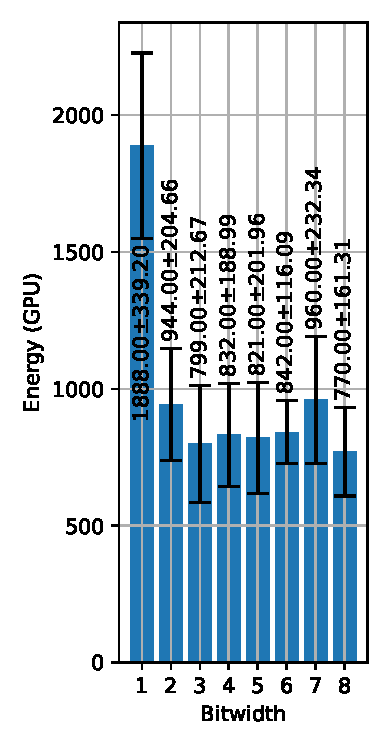
\includegraphics[width=\textwidth]{../standard/FashionMNIST/plots/fashionmnist_train_energy_gpu.pdf}
                \caption{Energy Consumption Estimation, Unit in Constant $c$}
            \end{subfigure}
            \hfill
            \begin{subfigure}[H]{0.48\textwidth}
                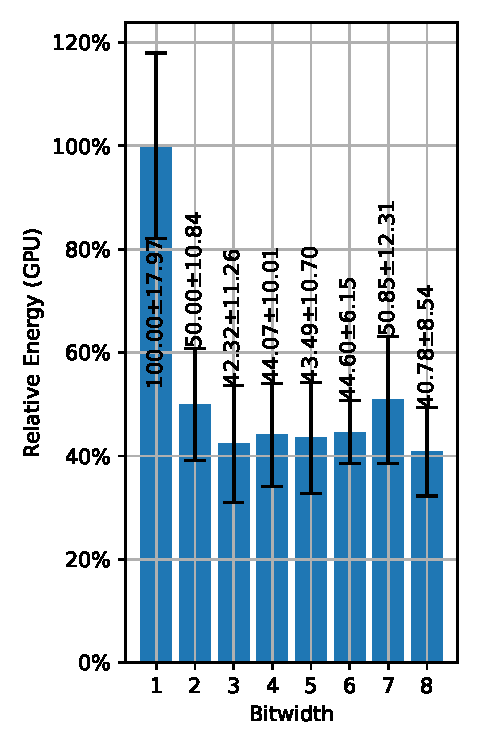
\includegraphics[width=\textwidth]{../standard/FashionMNIST/plots/fashionmnist_train_relative_energy_gpu.pdf}
                \caption{Normalized Energy Consumption Estimation Relative to 1-bit Spike Train Model}
            \end{subfigure}
            \caption{Training Energy Consumption Estimation on GPUs for Fashion MNIST Dataset}
            \label{fig:training_energy_gpu}
        \end{figure}

    \subsection{Inference Energy Consumption on Neuromorphic Chips}
    \label{subsec:inference_energy}
        A widely adopted energy estimation model for neuromorphic chips is the following:
        \begin{equation}
            \label{eq:inference_energy_popular}
            E_{\text{inference}} = F \cdot fr \cdot E_{\text{AC}} \cdot T
        \end{equation}
        where $F$ is the number of floating point operations required to simulate the network, $fr$ is the firing rate of the neurons, $E_{\text{AC}}$ is the energy consumption of accumulation, and $T$ is the number of time steps. 
    
        It is however hard to evaluate the energy consumption of the multi-bit spike train model on neuromorphic chips like Loihi and TrueNorth, as they do not support multi-bit spikes natively. Although it may be possible to encode the multi-bit spikes into multiple spikes with different intensities, the energy consumption of such encoding is very expensive due to the high cost of the synchronization barrier between the time steps. 

        A viable option is to consider hardware like Intel Loihi 2 which supports graded spikes up to 32-bit precision. We consider the case of Intel Loihi 2 and make the following assumptions: 
        \begin{enumerate}
            \item There is no difference in the energy consumption for the number of bits used to encode the spikes.
            \item The energy consumption for a floating point operation is always $E_{\text{MAC}}$ (Multiply-Accumulate).
        \end{enumerate}
        Since the payload is not variable in this case, the energy consumption of the multi-bit spike train model is directly proportional to the firing rate given fixed maximum floating point operations and time steps. Analog as the equation \ref{eq:inference_energy_popular}, we have the following estimation for the $i$-bit spike train model:
        \begin{equation}
            E_{\text{inference}-i} = F \cdot fr_i \cdot E_{\text{MAC}} \cdot T_i
        \end{equation}
        We can estimate the energy consumption of the 2-bit spike train model relative to the 1-bit spike train model by comparing the firing rate of the neurons. As expected, the energy consumption of the multi-bit spike train model is higher than the 1-bit spike train model, as the firing rate of the neurons is higher (see Figure \ref{fig:inference_energy_nh}).
        \begin{figure}[!htpb]
            \centering
            \begin{subfigure}[H]{\textwidth}
                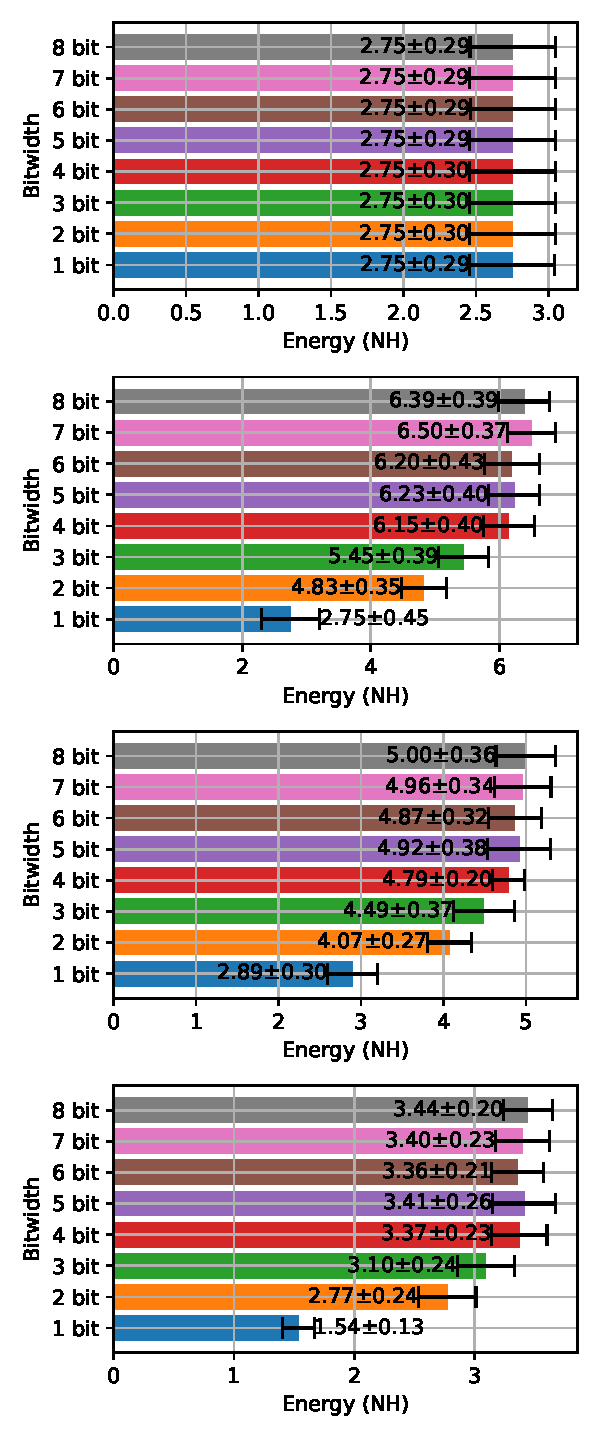
\includegraphics[width=\textwidth]{../standard/FashionMNIST/plots/fashionmnist_test_energy_nh.pdf}
                \caption{Energy Consumption Estimation, Unit in Parameters $F\cdot E_{\text{MAC}}$}
            \end{subfigure}
            \hfill
            \begin{subfigure}[H]{\textwidth}
                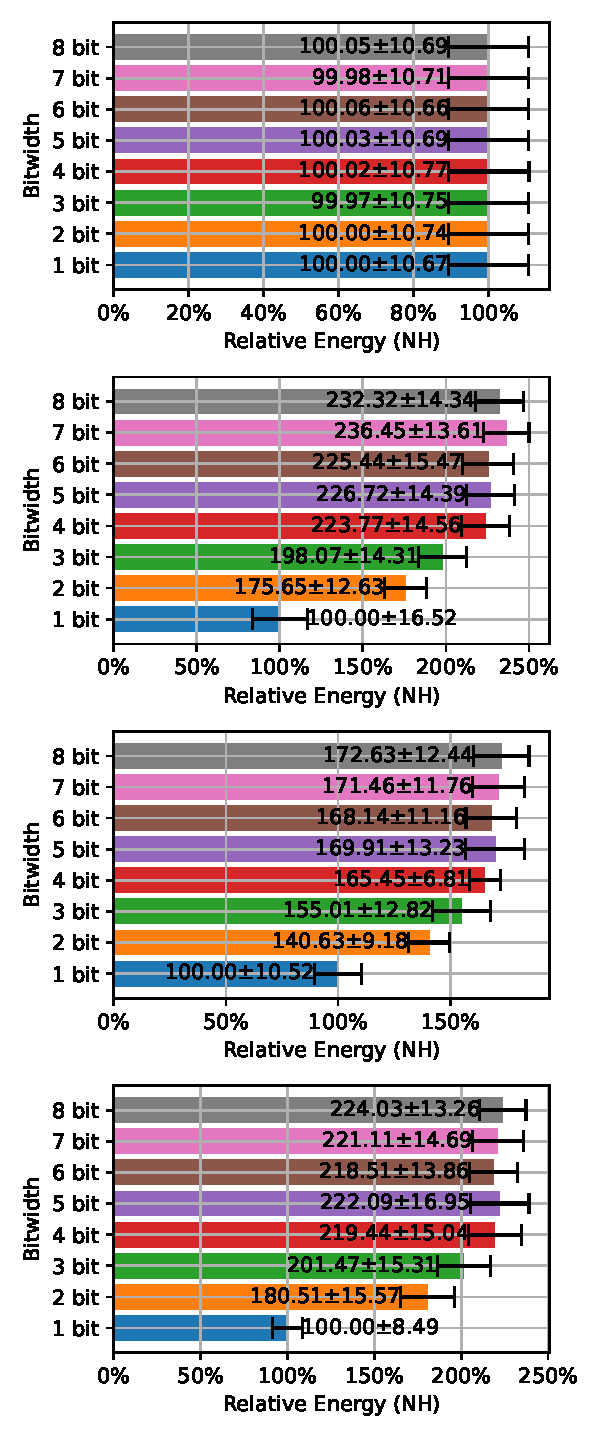
\includegraphics[width=\textwidth]{../standard/FashionMNIST/plots/fashionmnist_test_relative_energy_nh.pdf}
                \caption{Normalized Energy Consumption Estimation Relative to 1-bit Spike Train Model}
            \end{subfigure}
            \caption{Inference Energy Consumption Estimation on Intel Loihi 2 for Fashion MNIST Dataset}
            \label{fig:inference_energy_nh}
        \end{figure}
        %TODO: Add more figures in appendix
        %TODO: Add references to the analysis model

    \subsection{Tradeoffs}
        One can tell that the energy consumption of the multi-bit spike train model has no direct advantage over the 1-bit spike train model on neuromorphic chips, as the firing rate of the multi-bit spike train model tends to be higher than the 1-bit spike train model. Moreover, one can also argue that the energy consumption from $E_{\text{MAC}}$ is due to the graded spikes, which is not an issue with binary spikes. 

        We consider the energy consumption of the multi-bit spike train model in general as an opportunity to enable tradeoffs. If the inference is not the bottleneck of the application, then one can rely on the fast convergence speed of the multi-bit spike train model during training. If the inference is the bottleneck, then one can choose to train the multi-bit spike train model for longer time to achieve a firing rate that is comparable to the 1-bit spike train model (see Figure \ref{fig:inference_energy_nh_firerate}). Such tradeoffs are not possible with the 1-bit spike train model. 
        \begin{figure}[!htpb]
            \centering
            \begin{subfigure}[H]{0.48\textwidth}
                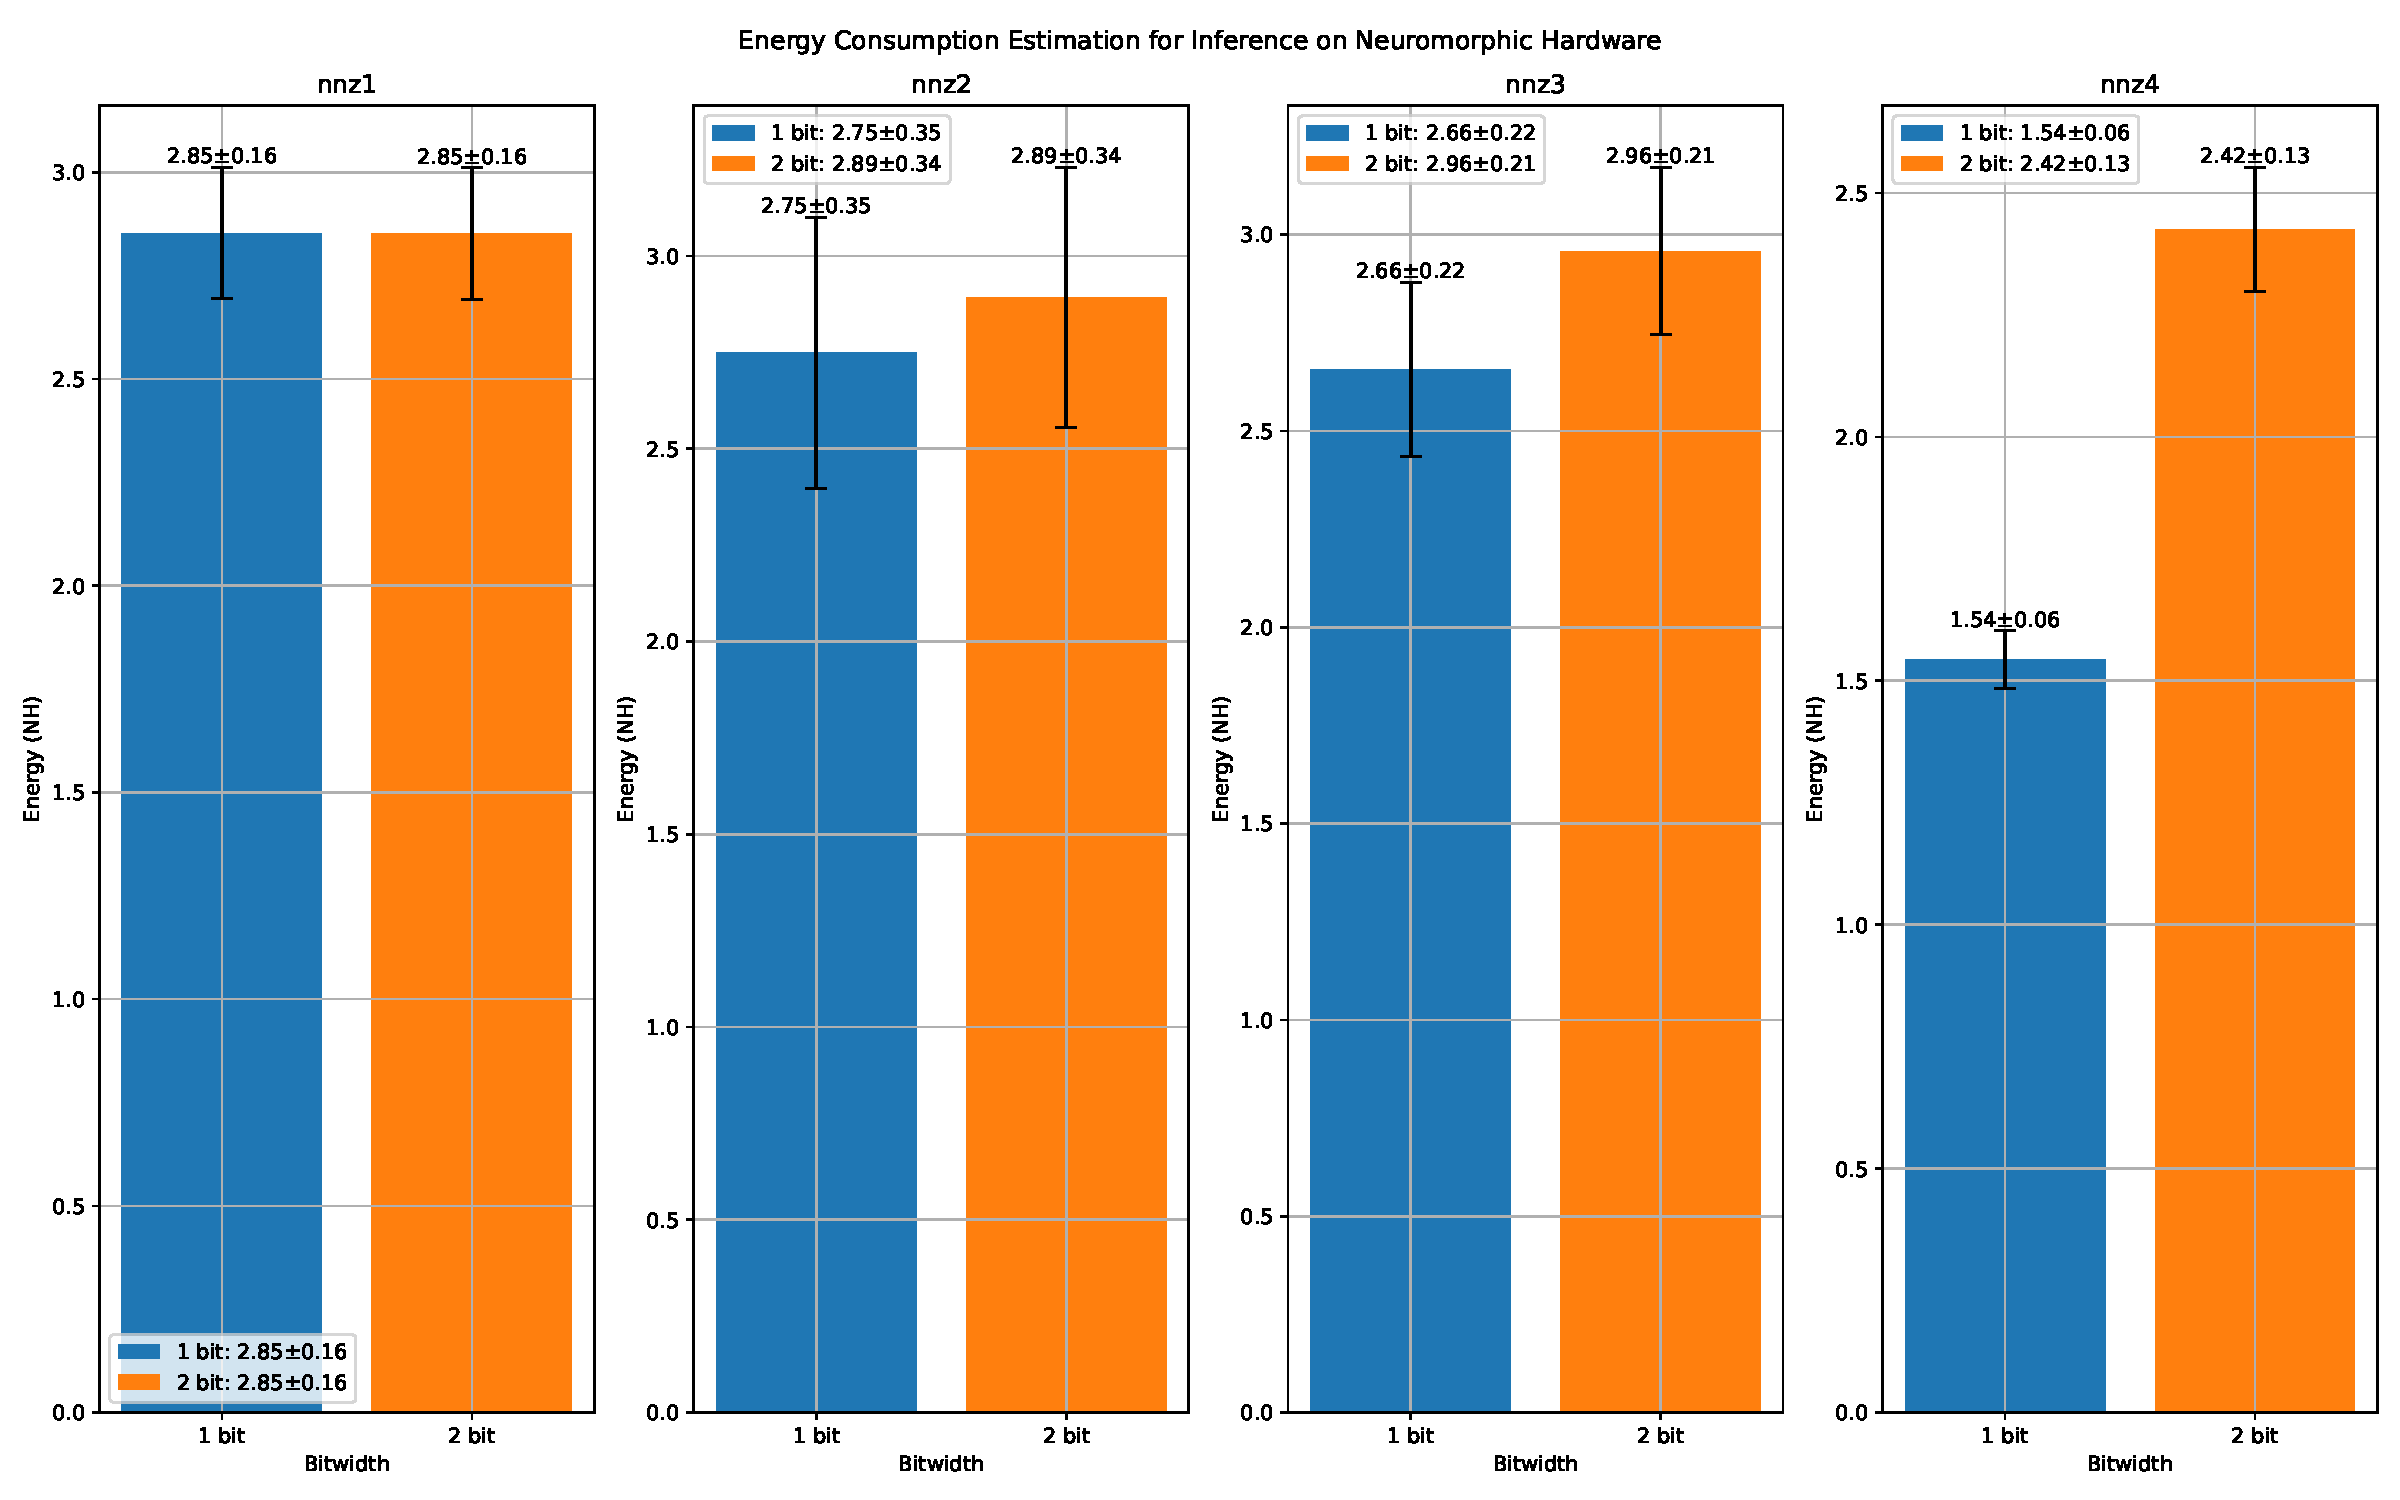
\includegraphics[width=\textwidth]{../firerate/FashionMNIST/plots/fashionmnist_test_energy_nh.pdf}
                \caption{Energy Consumption Estimation, Unit in Parameters $F\cdot E_{\text{MAC}}$}
            \end{subfigure}
            \hfill
            \begin{subfigure}[H]{0.48\textwidth}
                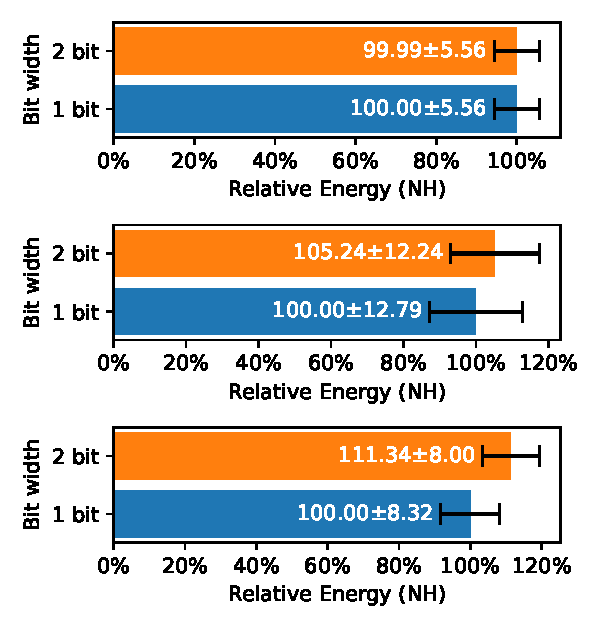
\includegraphics[width=\textwidth]{../firerate/FashionMNIST/plots/fashionmnist_test_relative_energy_nh.pdf}
                \caption{Normalized Energy Consumption Estimation Relative to 1-bit Spike Train Model}
            \end{subfigure}
            \caption{Inference Energy Consumption Estimation on Intel Loihi 2 for Fashion MNIST Dataset with 50 Training Epochs}
            \label{fig:inference_energy_nh_firerate}
        \end{figure}

        And more interestingly, if one is satisfied with the accuracy of the 1-bit spike train model, then one can choose to train the multi-bit spike train model for fewer time steps. This can enable higher efficiency in both training and inference. 

        We take again the example of Fashion MNIST dataset, while $T=10$ is a good choice for both the 1-bit and 2-bit spike train model, we can reduce the time steps to $T=4$ for the 2-bit spike train model and still achieve a comparable accuracy (see \ref{fig:inference_energy_nh_timesteps}). 
        \begin{figure}[!htpb]
            \centering
            \begin{subfigure}[H]{0.48\textwidth}
                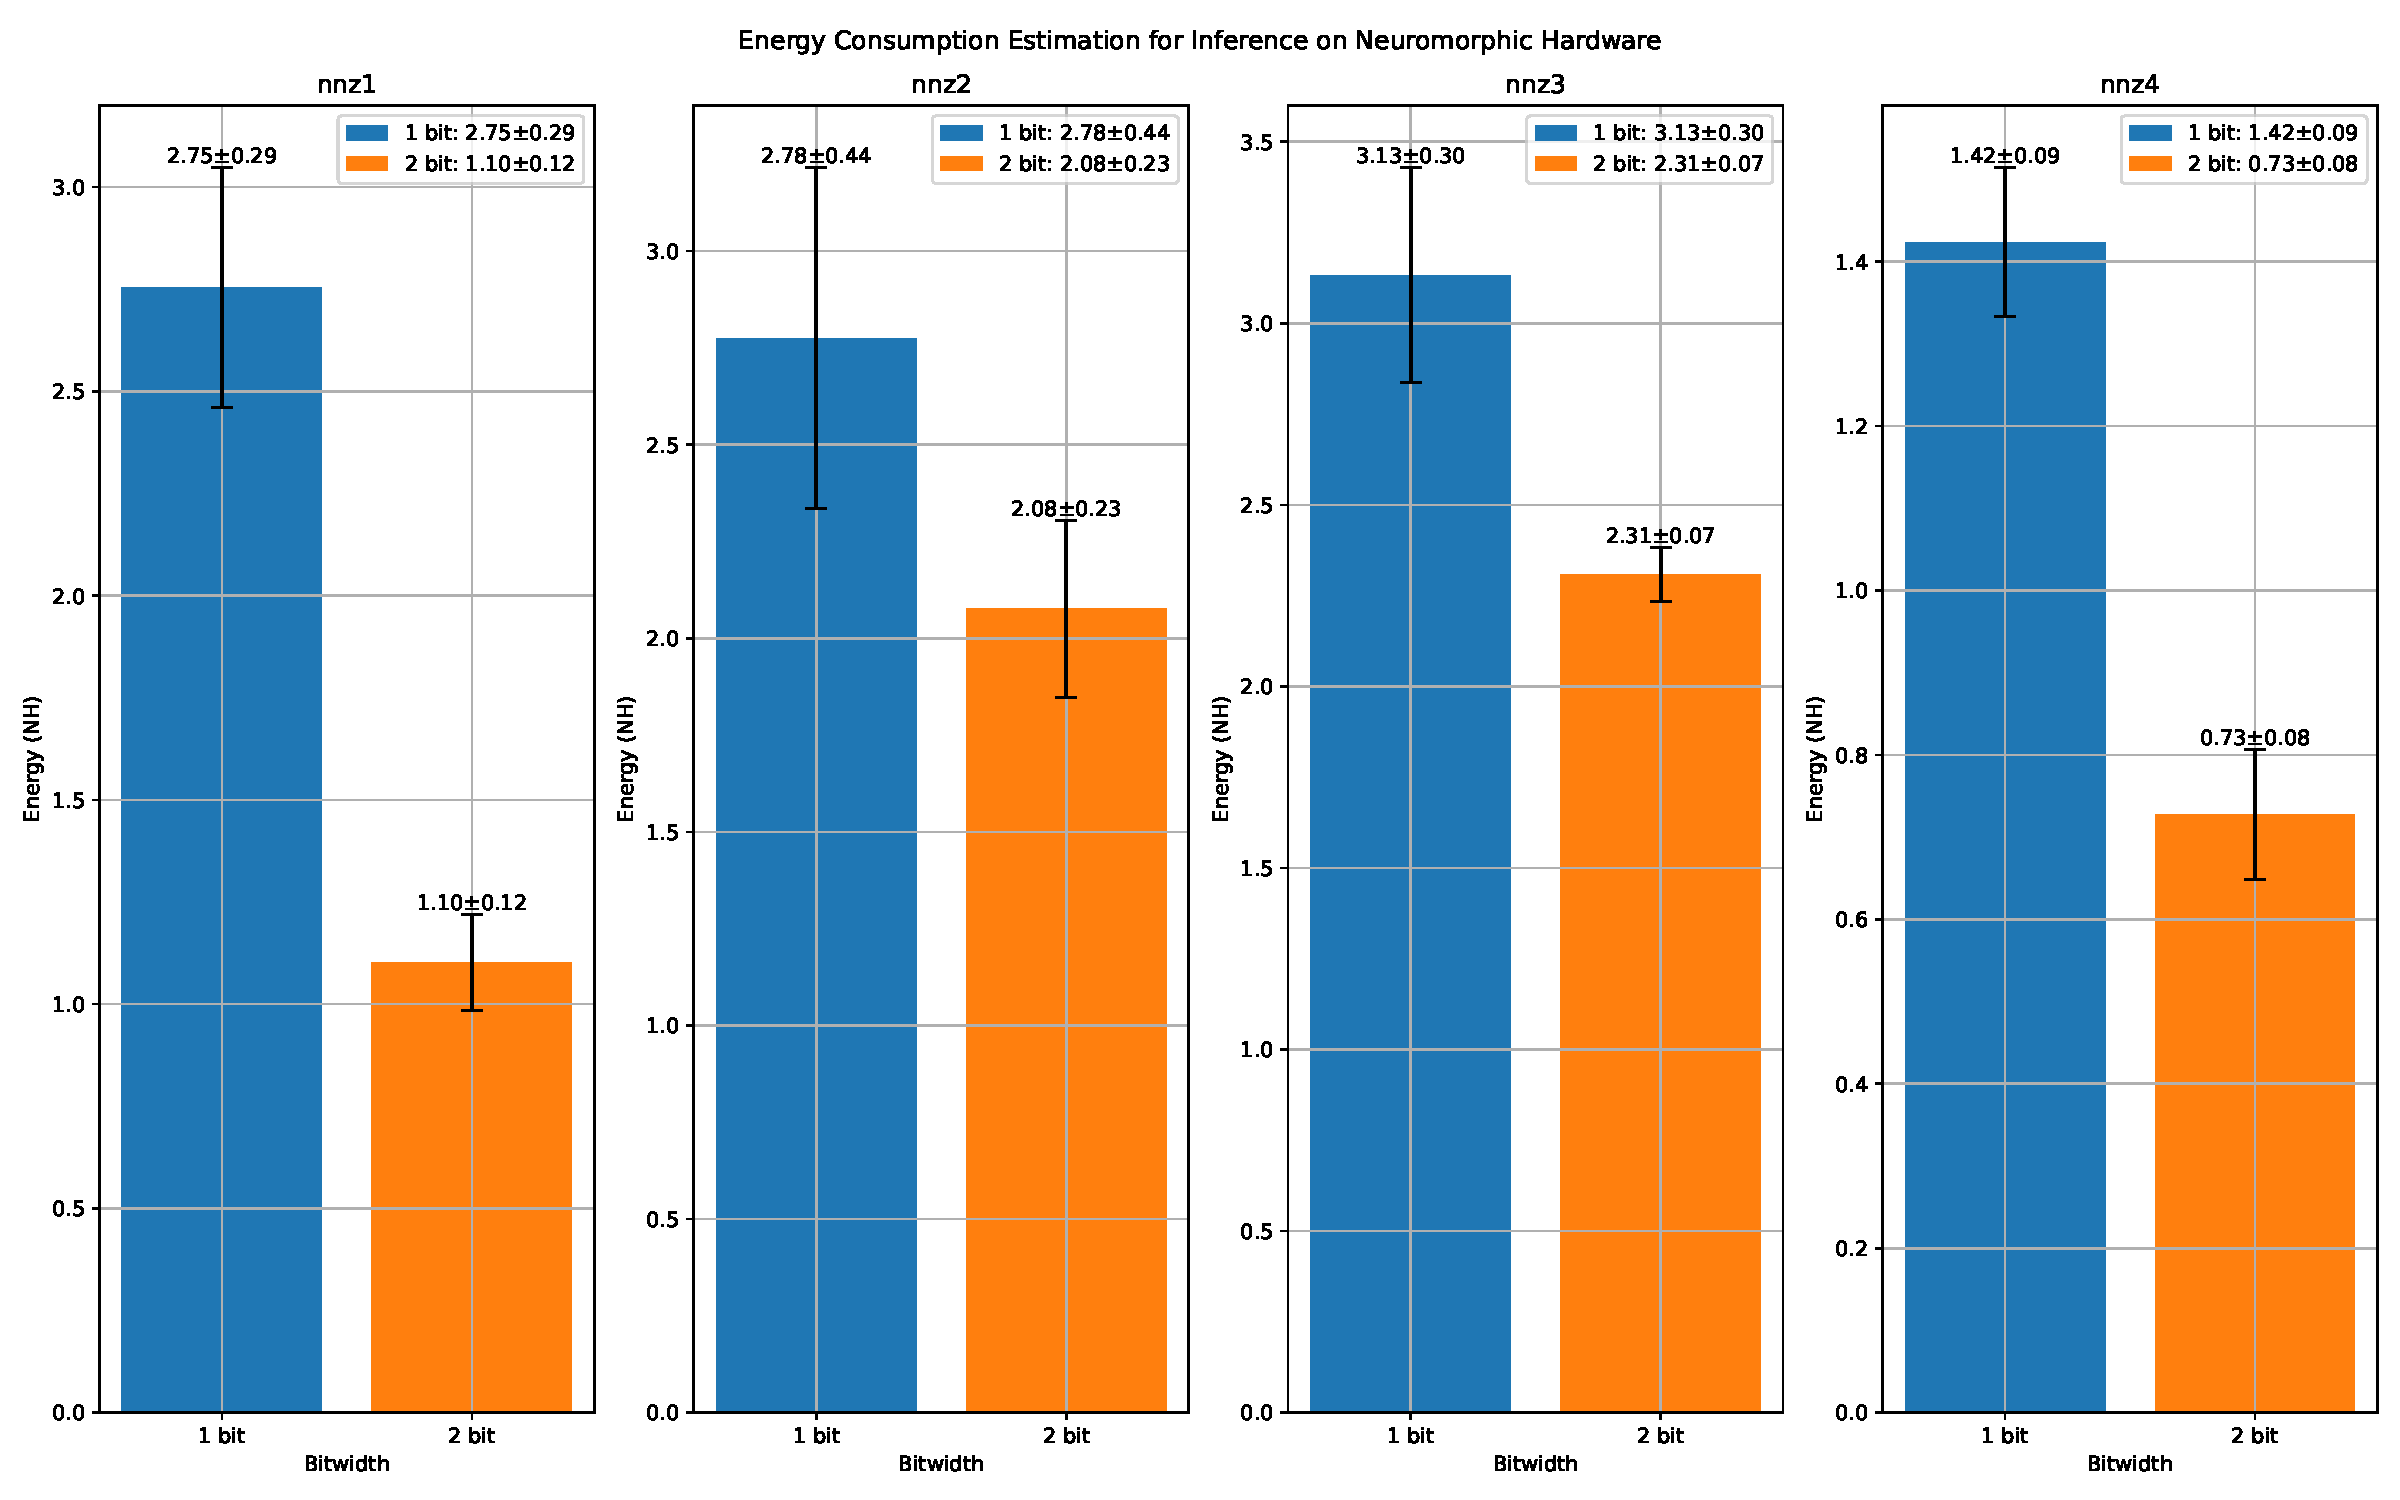
\includegraphics[width=\textwidth]{../timesteps/FashionMNIST/plots/fashionmnist_test_energy_nh.pdf}
                \caption{Energy Consumption Estimation, Unit in Parameters $F\cdot E_{\text{MAC}}$}
            \end{subfigure}
            \hfill
            \begin{subfigure}[H]{0.48\textwidth}
                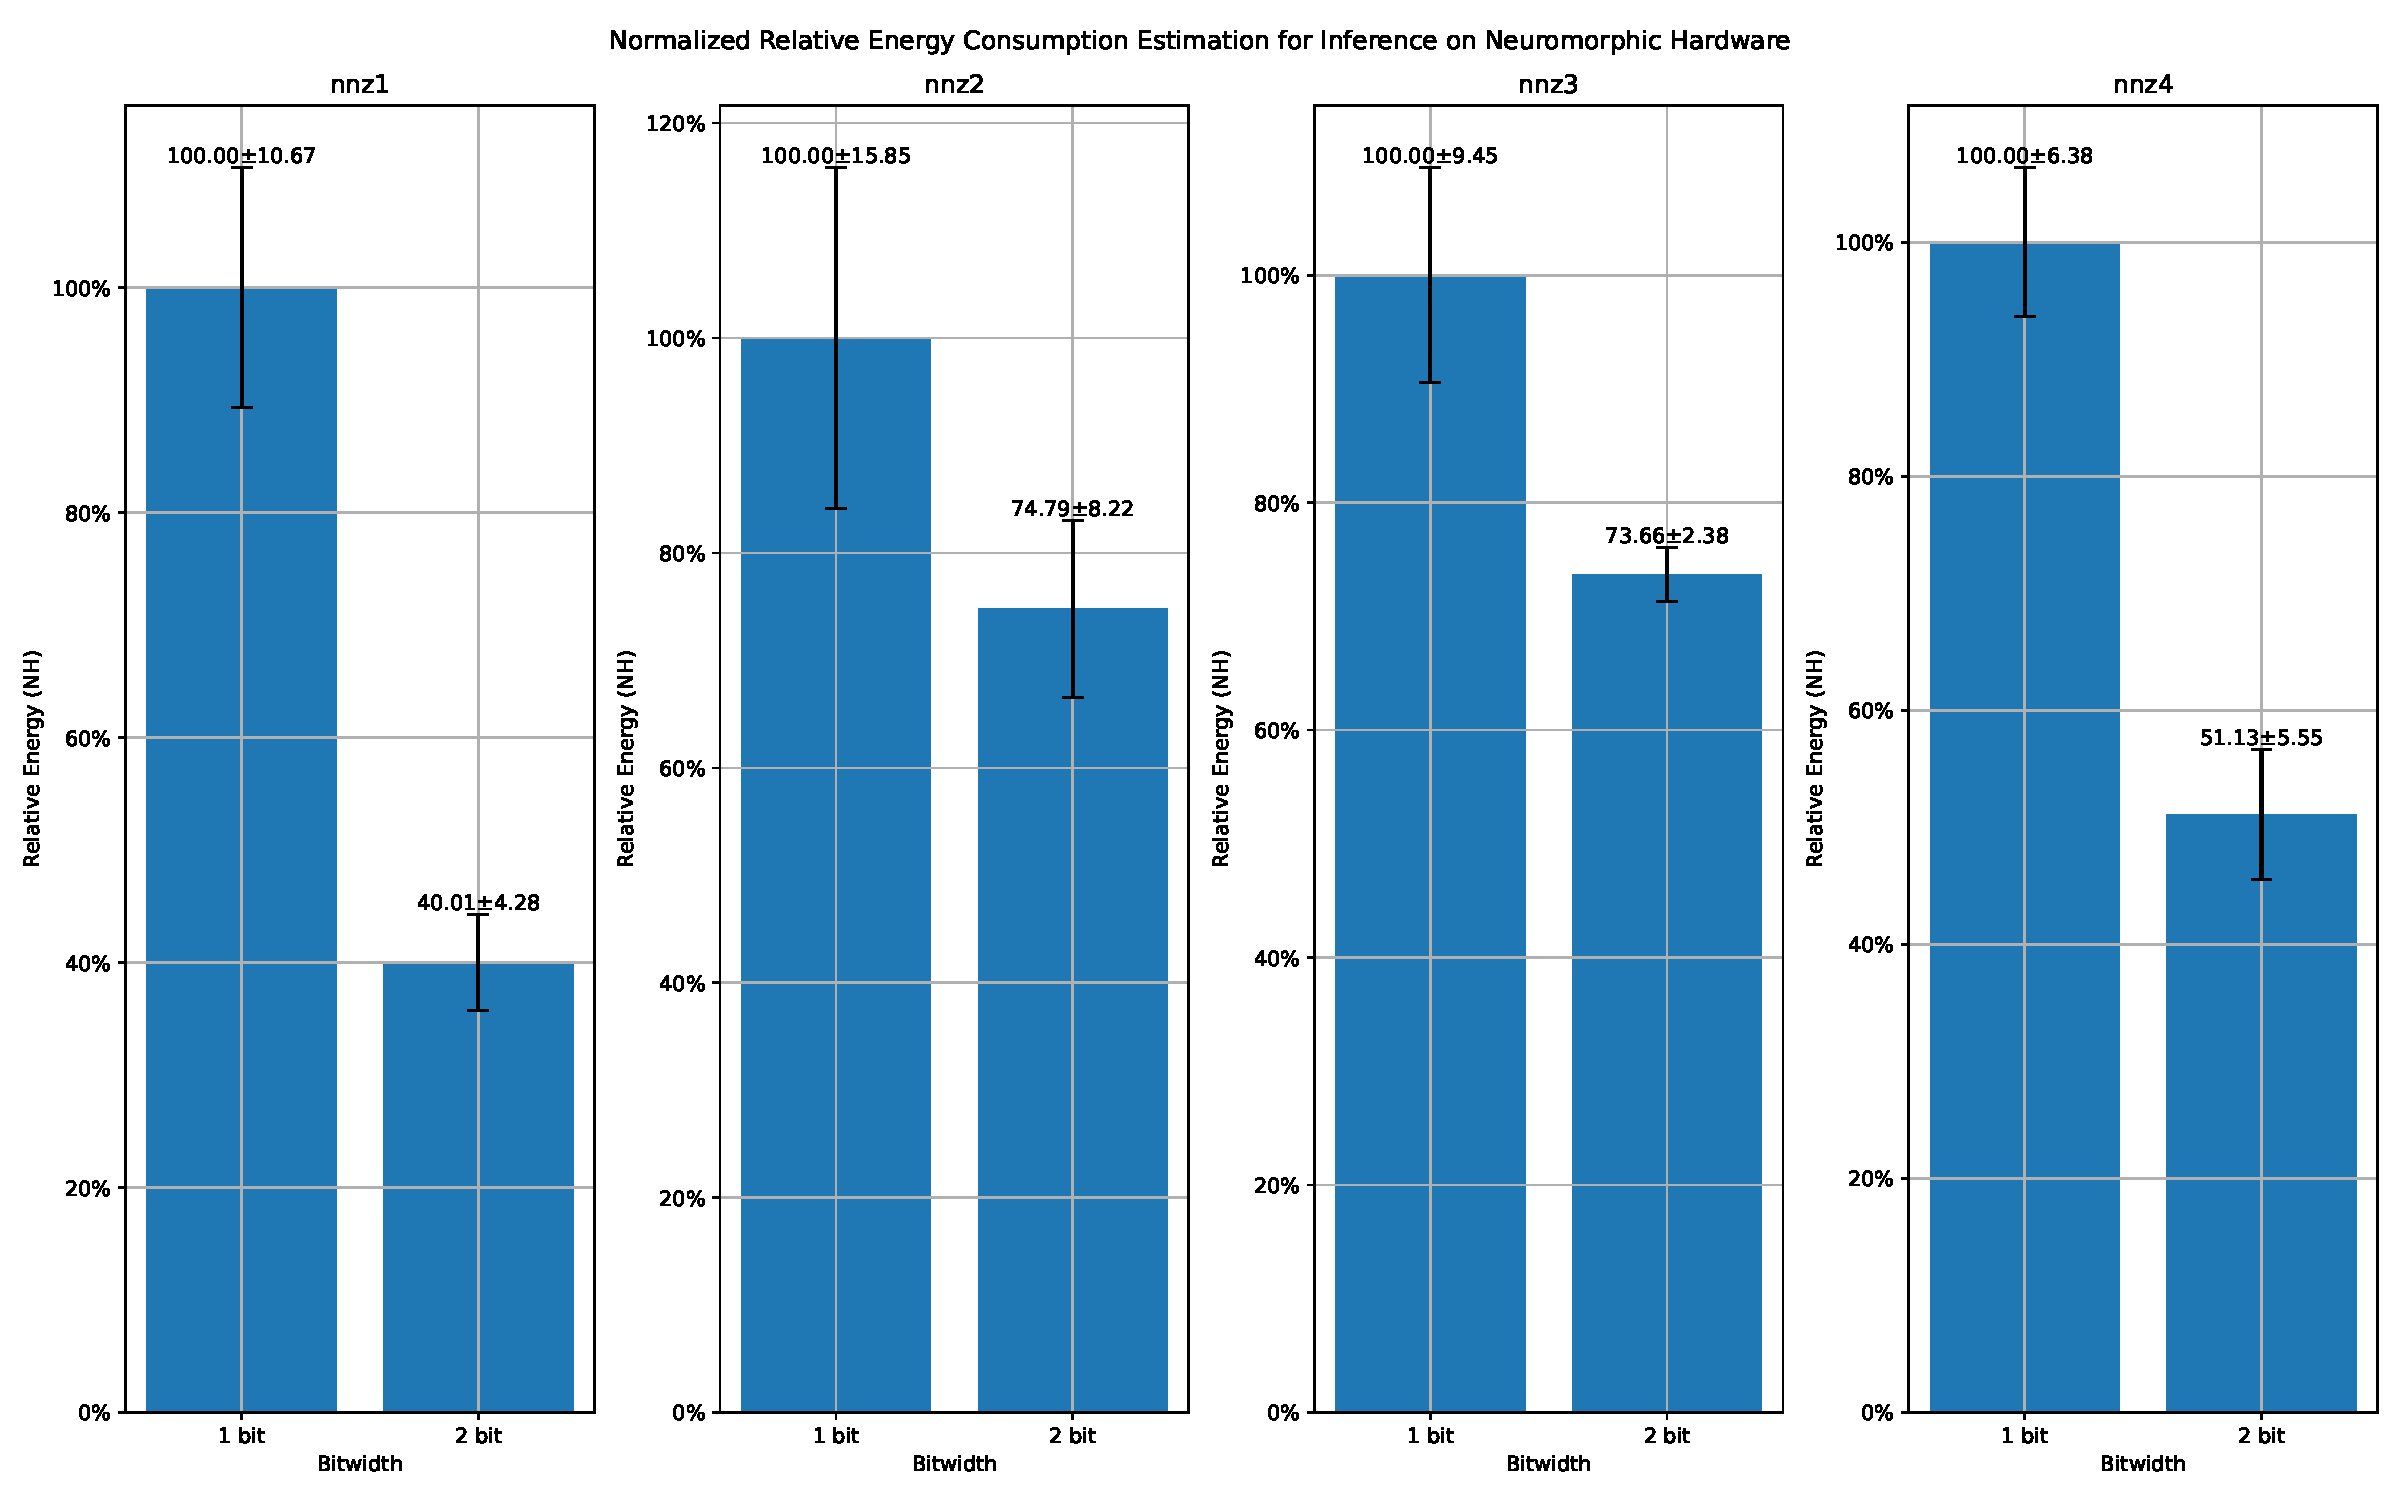
\includegraphics[width=\textwidth]{../timesteps/FashionMNIST/plots/fashionmnist_test_relative_energy_nh.pdf}
                \caption{Normalized Energy Consumption Estimation Relative to 1-bit Spike Train Model}
            \end{subfigure}
            \hfill
            \begin{subfigure}[H]{\textwidth}
                \centering
                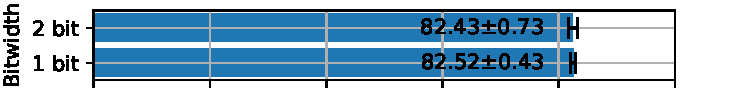
\includegraphics[width=\textwidth]{../timesteps/FashionMNIST/plots/fashionmnist_final_acc.pdf}
                \caption{Accuracy Comparison}
            \end{subfigure}
            \caption{Inference Energy Consumption Estimation on Intel Loihi 2 and Test Accuracy for Fashion MNIST Dataset with 10 Time Steps for 1-bit Spike Train Model and 4 Time Steps for 2-bit Spike Train Model}
            \label{fig:inference_energy_nh_timesteps}
        \end{figure}
        %TODO: Add more figures in appendix

        This can lead to a significant reduction in the energy consumption. It may not be reflected as a direct advantage in the energy consumption model mentioned above \ref{subsec:inference_energy}, but in practice, it should bring significant benefits, as most of the neuromorphic chips are designed to utilize the asynchronous communication via spikes, so they do not have a central clock system to synchronize the time steps very efficiently, and the cost for the synchronization barrier is very high. As reference, the latency per tile hop on Intel Loihi is at most around 6.5 ns where as the latency for the synchronization barrier is from 113-465 ns.
        %TODO: Add numbers from Intel Loihi.


\section{Performance}
\label{sec:performance}
    In the section \ref{subsec:training_energy}, we claim that the energy consumption on the GPUs are not affected by the firing rate and the bit width of the spike train in theory. However, in practice, with the increase of the bit width of the spike train, the training process slows down. This can be caused by the inefficient implementation of the multi-bit spike train model and the low level optimization on operations of sparse matrix multiplication. 
    % TODO: Measure the time consumption of multi-bit spike train model and 1-bit spike train model
    % TODO: Try JIT compilation? 
    There is sufficient room for improvement, e.g. by utilizing the sparsity of the spike trains or completely switching to the vectorized model instead of the temporal model instead, which is shown to be more efficient with learning algorithms like SLAYER and EXODUS. 
    % TODO: Cite the SLAYER and EXODUS papers
\chapter{Related Work}
\label{chap:related}

We mainly used the LIF neuron model \cite{lapicque1907louis} in this thesis, which is a simple model that does not capture the full complexity of biological neurons. Hudgkin and Huxley \cite{jphysiol.1952.sp004764} proposed a more detailed model that includes the dynamics of the ion channels, which is more biologically plausible but also computationally more expensive. Most of the models, e.g. Izhikevich's model \cite{1257420}, focus on some specific dynamics of the biological neurons and enable some tradeoffs. 

Although BPTT is widely used in training deep large SNNs, other methods such as spike-timing-dependent plasticity (STDP) \cite{doi:10.1126/science.275.5297.213} are more biologically plausible with clear evidence in the brain. Methods like SLAYER \cite{Shrestha2018} and EXODUS \cite{bauer2022exodus} focus more on the efficient computation of the gradients in the SNNs instead of the biological plausibility.

Typical constructions of SNNs include replacing the ReLU activation function in ANNs with the LIF neuron node. Due to the non-differentiability of the spike function and the time dependency of the membrane potential, the training of SNNs is more challenging than ANNs. Many methods, e.g. Spike-Norm \cite{10.3389/fnins.2019.00095} and Spiking RWKV \cite{zhu2024spikegptgenerativepretrainedlanguage} focus on replacing some components of ANNs with certain tweaks for SNNs to maintain the performance witnessed in ANNs while easing the training process.

As the demand for AI applications grows, the energy efficiency of the hardware becomes more important. Neuromorphic hardwares like IBM's TrueNorth \cite{7229264} and Intel's Loihi \cite{8259423} are designed to exploit the fact that within a discrete time step, there is no need for synchronous communication between the neurons, as each spike increases the membrane potential of the target neuron and such operation is commutative. This allows a partially asynchronous hardware design that can be more energy efficient than traditional GPUs. 
However, they lack the capability of training the network on the hardware, which is still done on traditional GPUs.

Quantization is a technique to reduce the memory footprint and computation cost of the neural networks by reducing the precision of the parameters. While large language models implemented in ANNs can be quantized to 4-bit precision \cite{ashkboos2024quarotoutlierfree4bitinference}, SNNs can be quantized to even lower precision \cite{10.1145/3664647.3681186} which should be able to achieve higher energy efficiency.

There exists work that shows the potential of using multi-bit spike trains in SNNs. In \cite{xiao2024multibitmechanismnovelinformation} the authors propose to use two integer number of bits to describe the ratio of the membrane potential to the threshold. They were able to show that the multi-bit spike train model can achieve better accuracy. 
Our work differs from \cite{xiao2024multibitmechanismnovelinformation} in that we divide the range of the membrane potential into $2^n-1$ intervals and center the sigmoid function accordingly. This allows us to show the improvement in the convergence speed and the performance of the network.
\chapter{Concluding Remarks}
\label{chap:concluding_remarks}

    \section{Conclusion}
    \label{sec:conclusion}
        In this thesis we have developed a novel spike train model for spiking neural networks (SNNs) that uses multi-bit spikes to encode the information. We implement it using an SNN framework, SpikingJelly, based on PyTorch. And we have shown that the multi-bit spike train model can significantly improve the convergence speed and accuracy of the network compared to the traditional 1-bit spike train model while preserving other characteristics of the 1-bit spike train model such as high quantizability and low energy consumption. We consider the tradeoffs the multi-bit spike train model can bring in terms of energy consumption and performance important for maximizing the efficiency of SNNs on various hardware platforms.

        %TODO: Repeat the most important results here with numbers and statistics.

    \section{Future Work}
    \label{sec:future_work}
        The multi-bit spike train model is a promising direction for the development of SNNs. However, there are still many open questions and challenges that need to be addressed in the future. Here we list some of the possible future work:
        \begin{itemize}
            \item \textbf{Optimization of the multi-bit spike train model:} The current implementation of the multi-bit spike train model is not optimized for performance. One can consider using just-in-time (JIT) compilation to improve the performance of the model. 
            \item \textbf{Investigation of the overfitting problem:} The multi-bit spike train model is more complicated than the 1-bit spike train model, which can lead to overfitting. One can investigate the overfitting problem and propose solutions to mitigate it.
            \item \textbf{Extension to other tasks and datasets:} The experiments in this thesis are mainly focused on image classification tasks. One can extend the multi-bit spike train model to other tasks and datasets to evaluate its performance.
            \item \textbf{Implementation on neuromorphic chips:} The multi-bit spike train model is designed to be hardware-friendly in theory. It would be more convincing if one can implement the model on neuromorphic chips like Intel Loihi 2 to evaluate its performance on specialized hardware.
            \item \textbf{Investigation of the energy consumption model:} The energy consumption model presented in this thesis is a simple estimation. One can investigate the energy consumption of the multi-bit spike train model more thoroughly and propose a more accurate model. Ideally, one can also measure the energy consumption of the multi-bit spike train model after implementing it on neuromorphic chips.
        \end{itemize}

\appendix

\chapter{Accuracy of the Multi-Bit Spike Train Model}
\label{appendix:accuracy}

\section{Accuracy Curves}
\label{appendix:accuracy_curves}

    All train accuracy curves are smoothed with a window size of 100.

    The hyperparameters used in the training process are shown in Table \ref{tab:hyperparameters_accuracy}.

    \begin{table}[H]
        \begin{tabularx}{\textwidth}{|X|c|c|c|c|c|c|c|}
            \toprule
            Dataset & Reps & Epochs & LR & Opt & Batch & Time steps \\
            \midrule
            Fashion MNIST & 10 & 5 & 2e-3 & Adam & 128 & 10 \\
            MNIST & 10 & 5 & 2e-3 & Adam & 128 & 10 \\
            NMNIST & 10 & 5 & 2e-3 & Adam & 128 & 10 \\
            DVS Gesture & 10 & 20 & 1e-3 & Adam & 128 & 10 \\
            CIFAR-10 & 5 & 50 & 1e-5 & Adam & 128 & 10 \\
            \bottomrule
        \end{tabularx}
        \caption{Hyperparameters}
        \label{tab:hyperparameters_accuracy}
    \end{table}

    \label{appendix:accuracy_curves_fashion_mnist}
        % \begin{figure}[H]
        %     \centering
        %     \begin{subfigure}[H]{0.55\textwidth}
        %         \centering
        %         \begin{subfigure}[H]{\textwidth}
        %             \centering
        %             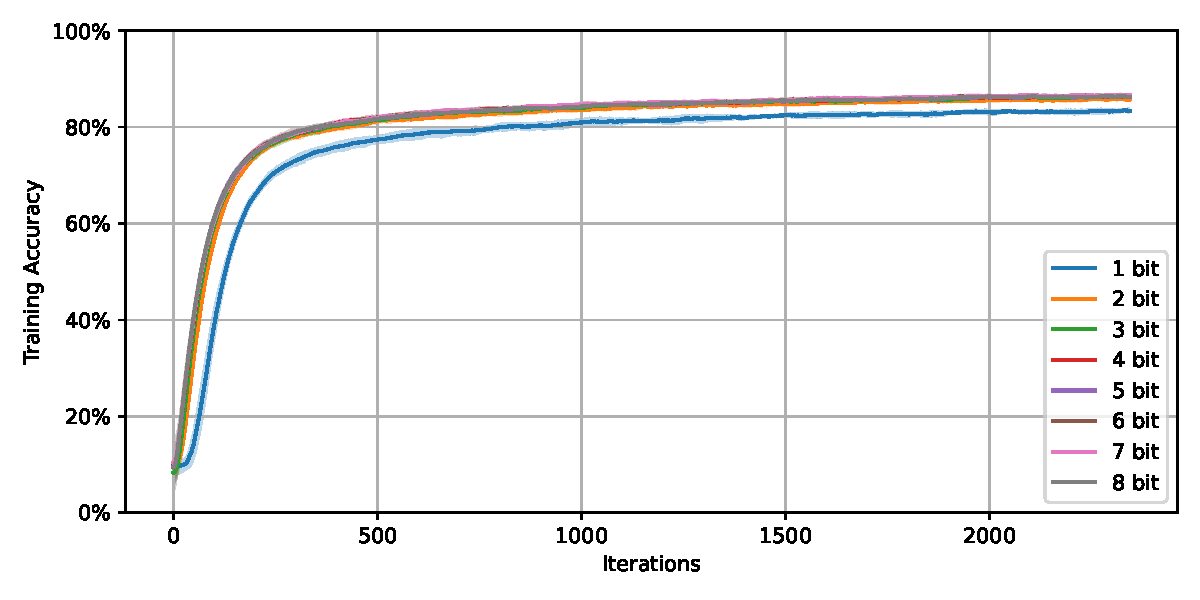
\includegraphics[width=\textwidth]{../standard/FashionMNIST/plots/fashionmnist_train_acc.pdf}
        %             \caption{Train Accuracy}
        %         \end{subfigure}
        %         \hfill
        %         \begin{subfigure}[H]{\textwidth}
        %             \centering
        %             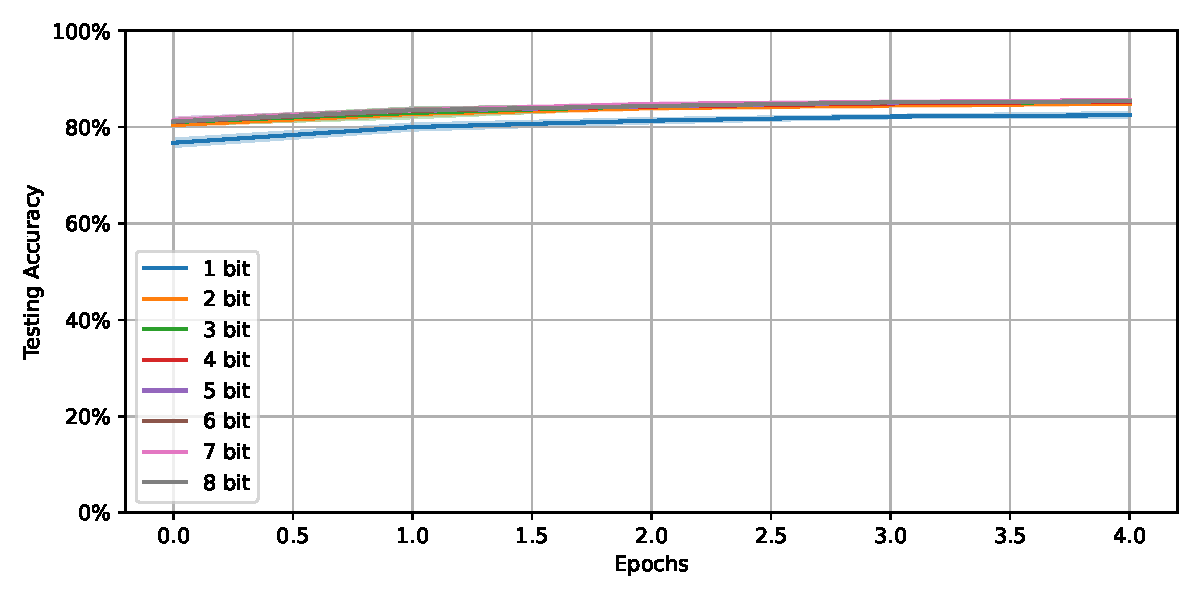
\includegraphics[width=\textwidth]{../standard/FashionMNIST/plots/fashionmnist_test_acc.pdf}
        %             \caption{Test Accuracy}
        %         \end{subfigure}
        %     \end{subfigure}
        %     \hfill
        %     \begin{subfigure}[H]{0.3\textwidth}
        %         \centering
        %         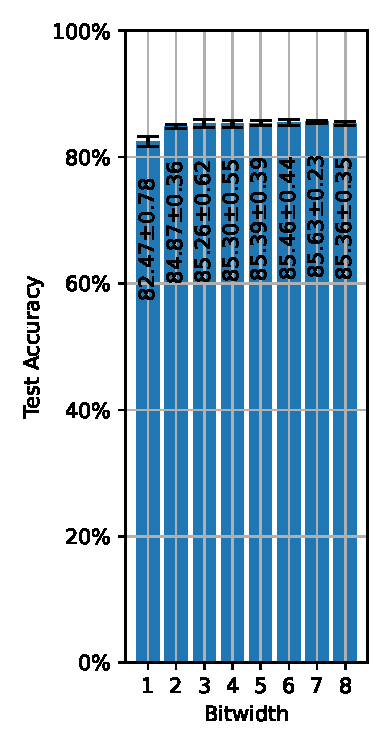
\includegraphics[width=\textwidth]{../standard/FashionMNIST/plots/fashionmnist_final_acc.pdf}
        %         \caption{Final Test Accuracy}
        %     \end{subfigure}
        %     \caption{Accuracy Curves of the Fashion MNIST Model}
        % \end{figure}
        \begin{figure}[H]
            \centering
            \begin{subfigure}[H]{\textwidth}
                \centering
                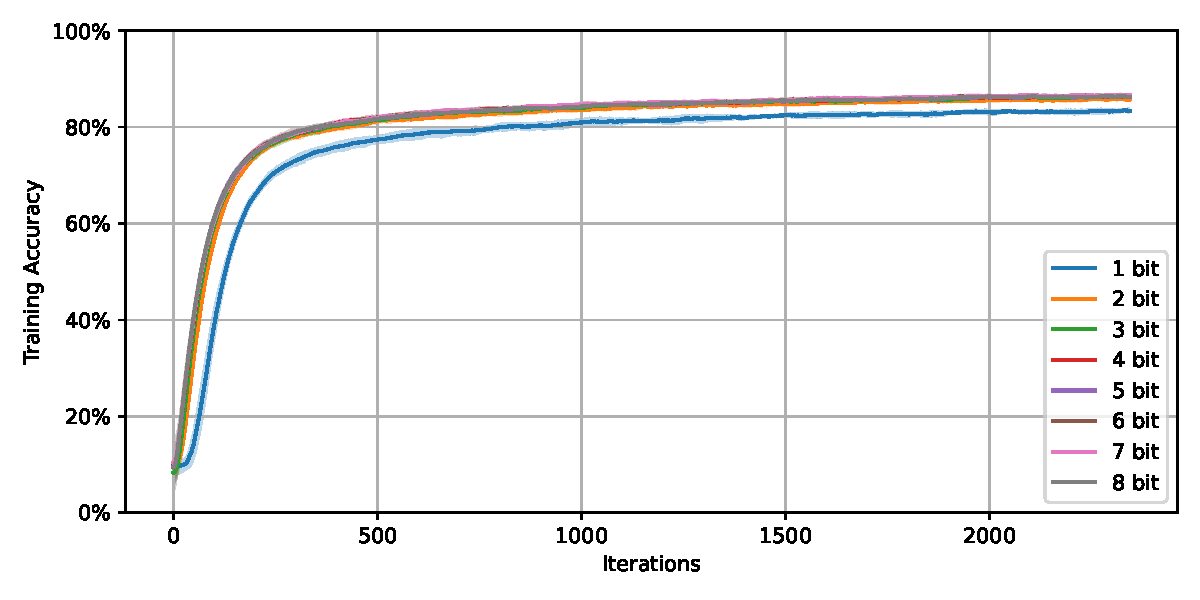
\includegraphics[width=\textwidth]{../standard/FashionMNIST/plots/fashionmnist_train_acc.pdf}
                \caption{Train Accuracy}
            \end{subfigure}
        \end{figure}
        \begin{figure}[H]
            \centering
            \ContinuedFloat
            \begin{subfigure}[H]{\textwidth}
                \centering
                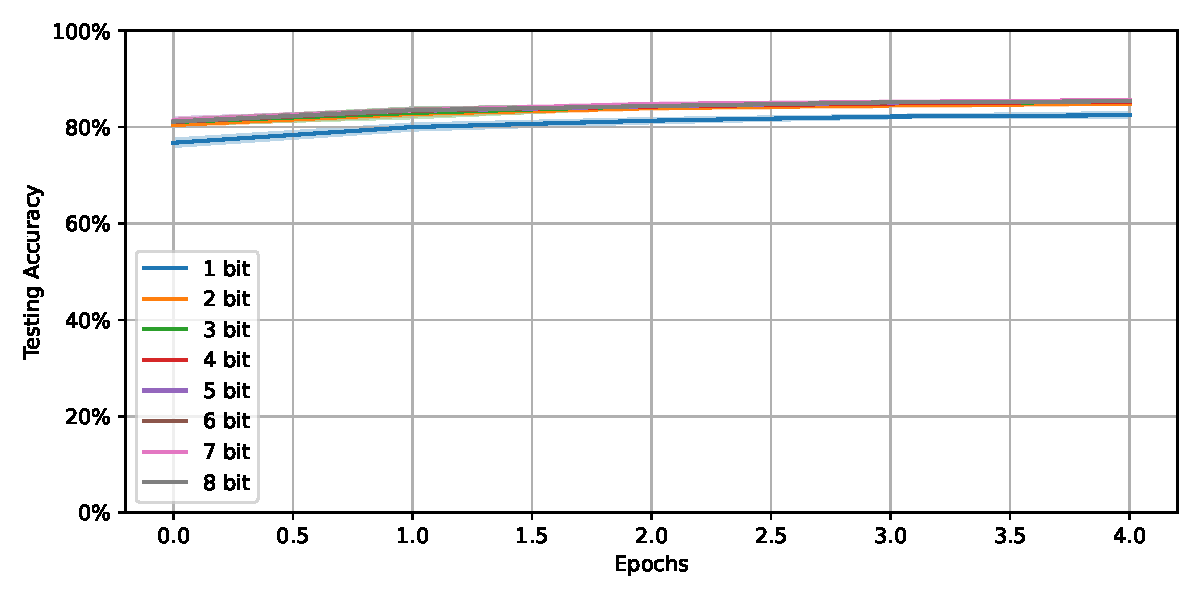
\includegraphics[width=\textwidth]{../standard/FashionMNIST/plots/fashionmnist_test_acc.pdf}
                \caption{Test Accuracy}
            \end{subfigure}
        \end{figure}
        \begin{figure}[H]
            \centering
            \ContinuedFloat
            \begin{subfigure}[H]{\textwidth}
                \centering
                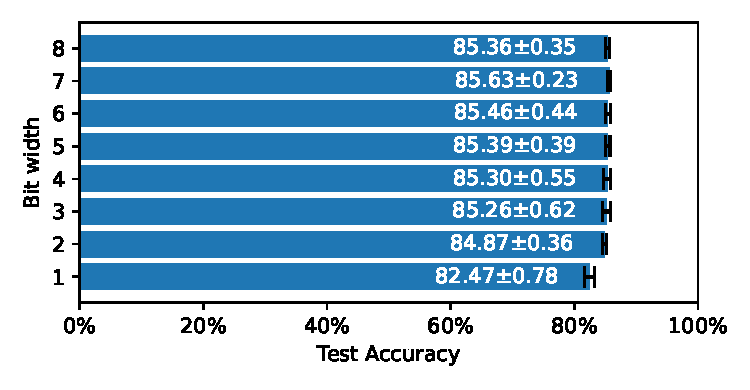
\includegraphics[width=\textwidth]{../standard/FashionMNIST/plots/fashionmnist_final_acc_horizontal.pdf}
                \caption{Final Test Accuracy}
            \end{subfigure}
            \caption{Accuracy Curves of the Fashion MNIST Model}
        \end{figure}

    \label{appendix:accuracy_curves_mnist}
        % \begin{figure}[H]
        %     \centering
        %     \begin{subfigure}[H]{0.55\textwidth}
        %         \centering
        %         \begin{subfigure}[H]{\textwidth}
        %             \centering
        %             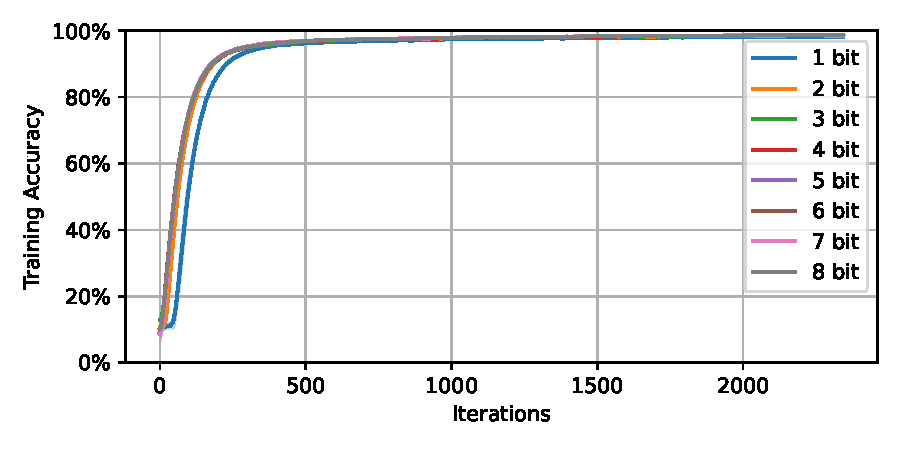
\includegraphics[width=\textwidth]{../standard/MNIST/plots/mnist_train_acc.pdf}
        %             \caption{Train Accuracy}
        %         \end{subfigure}
        %         \hfill
        %         \begin{subfigure}[H]{\textwidth}
        %             \centering
        %             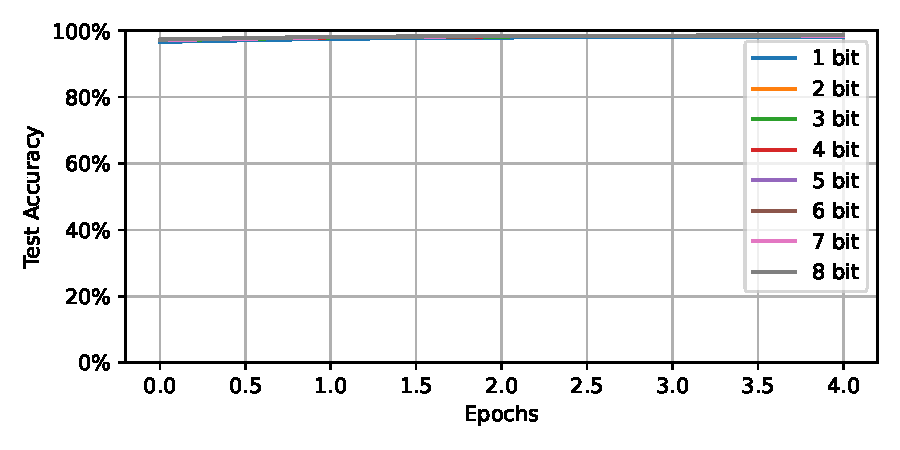
\includegraphics[width=\textwidth]{../standard/MNIST/plots/mnist_test_acc.pdf}
        %             \caption{Test Accuracy}
        %         \end{subfigure}
        %     \end{subfigure}
        %     \hfill
        %     \begin{subfigure}[H]{0.3\textwidth}
        %         \centering
        %         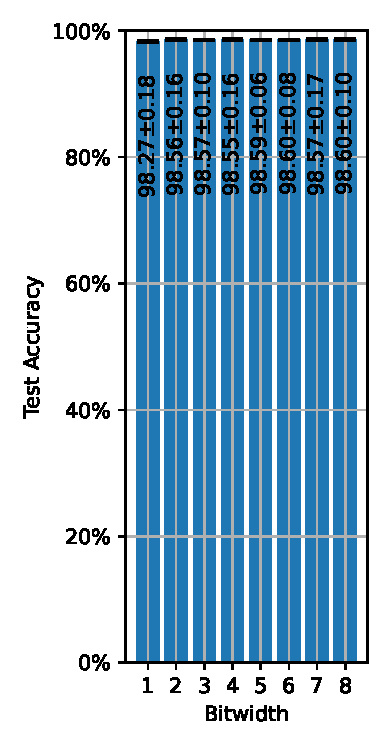
\includegraphics[width=\textwidth]{../standard/MNIST/plots/mnist_final_acc.pdf}
        %         \caption{Final Test Accuracy}
        %     \end{subfigure}
        %     \caption{Accuracy Curves of the MNIST Model}
        % \end{figure}
        \begin{figure}[H]
            \centering
            \begin{subfigure}[H]{\textwidth}
                \centering
                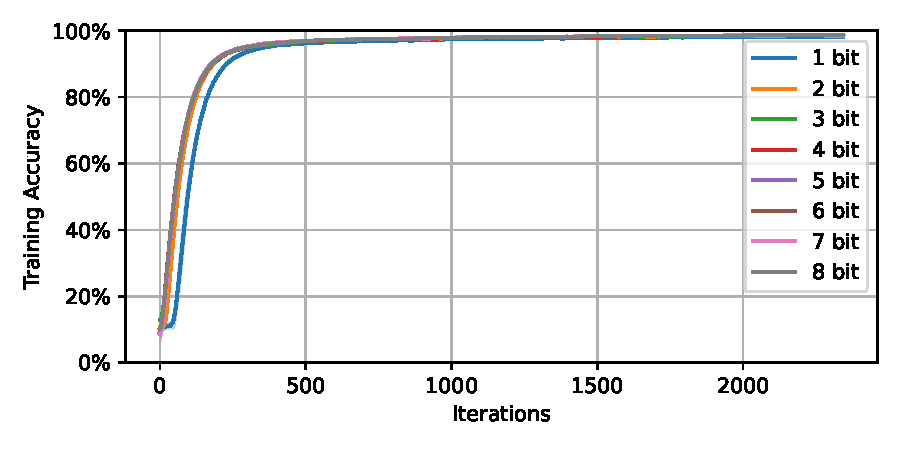
\includegraphics[width=\textwidth]{../standard/MNIST/plots/mnist_train_acc.pdf}
                \caption{Train Accuracy}
            \end{subfigure}
        \end{figure}
        \begin{figure}[H]
            \centering
            \ContinuedFloat
            \begin{subfigure}[H]{\textwidth}
                \centering
                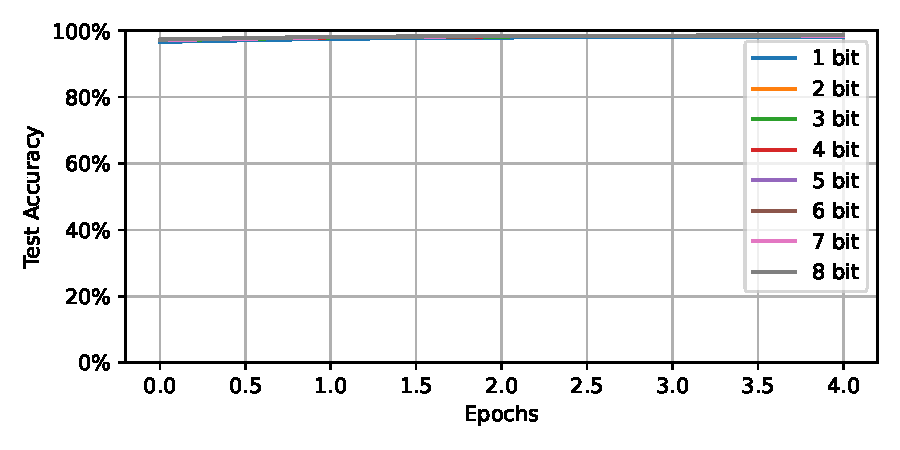
\includegraphics[width=\textwidth]{../standard/MNIST/plots/mnist_test_acc.pdf}
                \caption{Test Accuracy}
            \end{subfigure}
        \end{figure}
        \begin{figure}[H]
            \centering
            \ContinuedFloat
            \begin{subfigure}[H]{\textwidth}
                \centering
                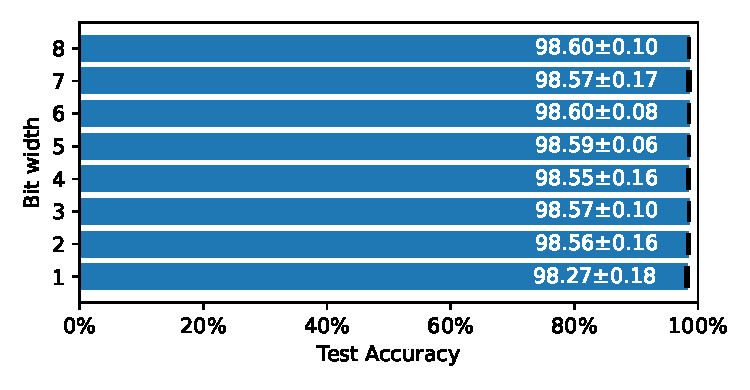
\includegraphics[width=\textwidth]{../standard/MNIST/plots/mnist_final_acc_horizontal.pdf}
                \caption{Final Test Accuracy}
            \end{subfigure}
            \caption{Accuracy Curves of the MNIST Model}
        \end{figure}
    
    \label{appendix:accuracy_curves_nmnist}
        % \begin{figure}[H]
        %     \centering
        %     \begin{subfigure}[H]{0.55\textwidth}
        %         \centering
        %         \begin{subfigure}[H]{\textwidth}
        %             \centering
        %             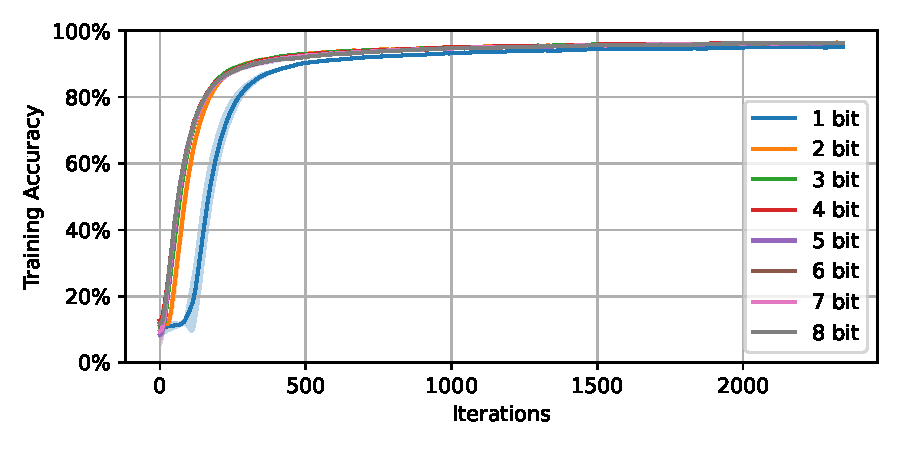
\includegraphics[width=\textwidth]{../standard/NMNIST/plots/nmnist_train_acc.pdf}
        %             \caption{Train Accuracy}
        %         \end{subfigure}
        %         \hfill
        %         \begin{subfigure}[H]{\textwidth}
        %             \centering
        %             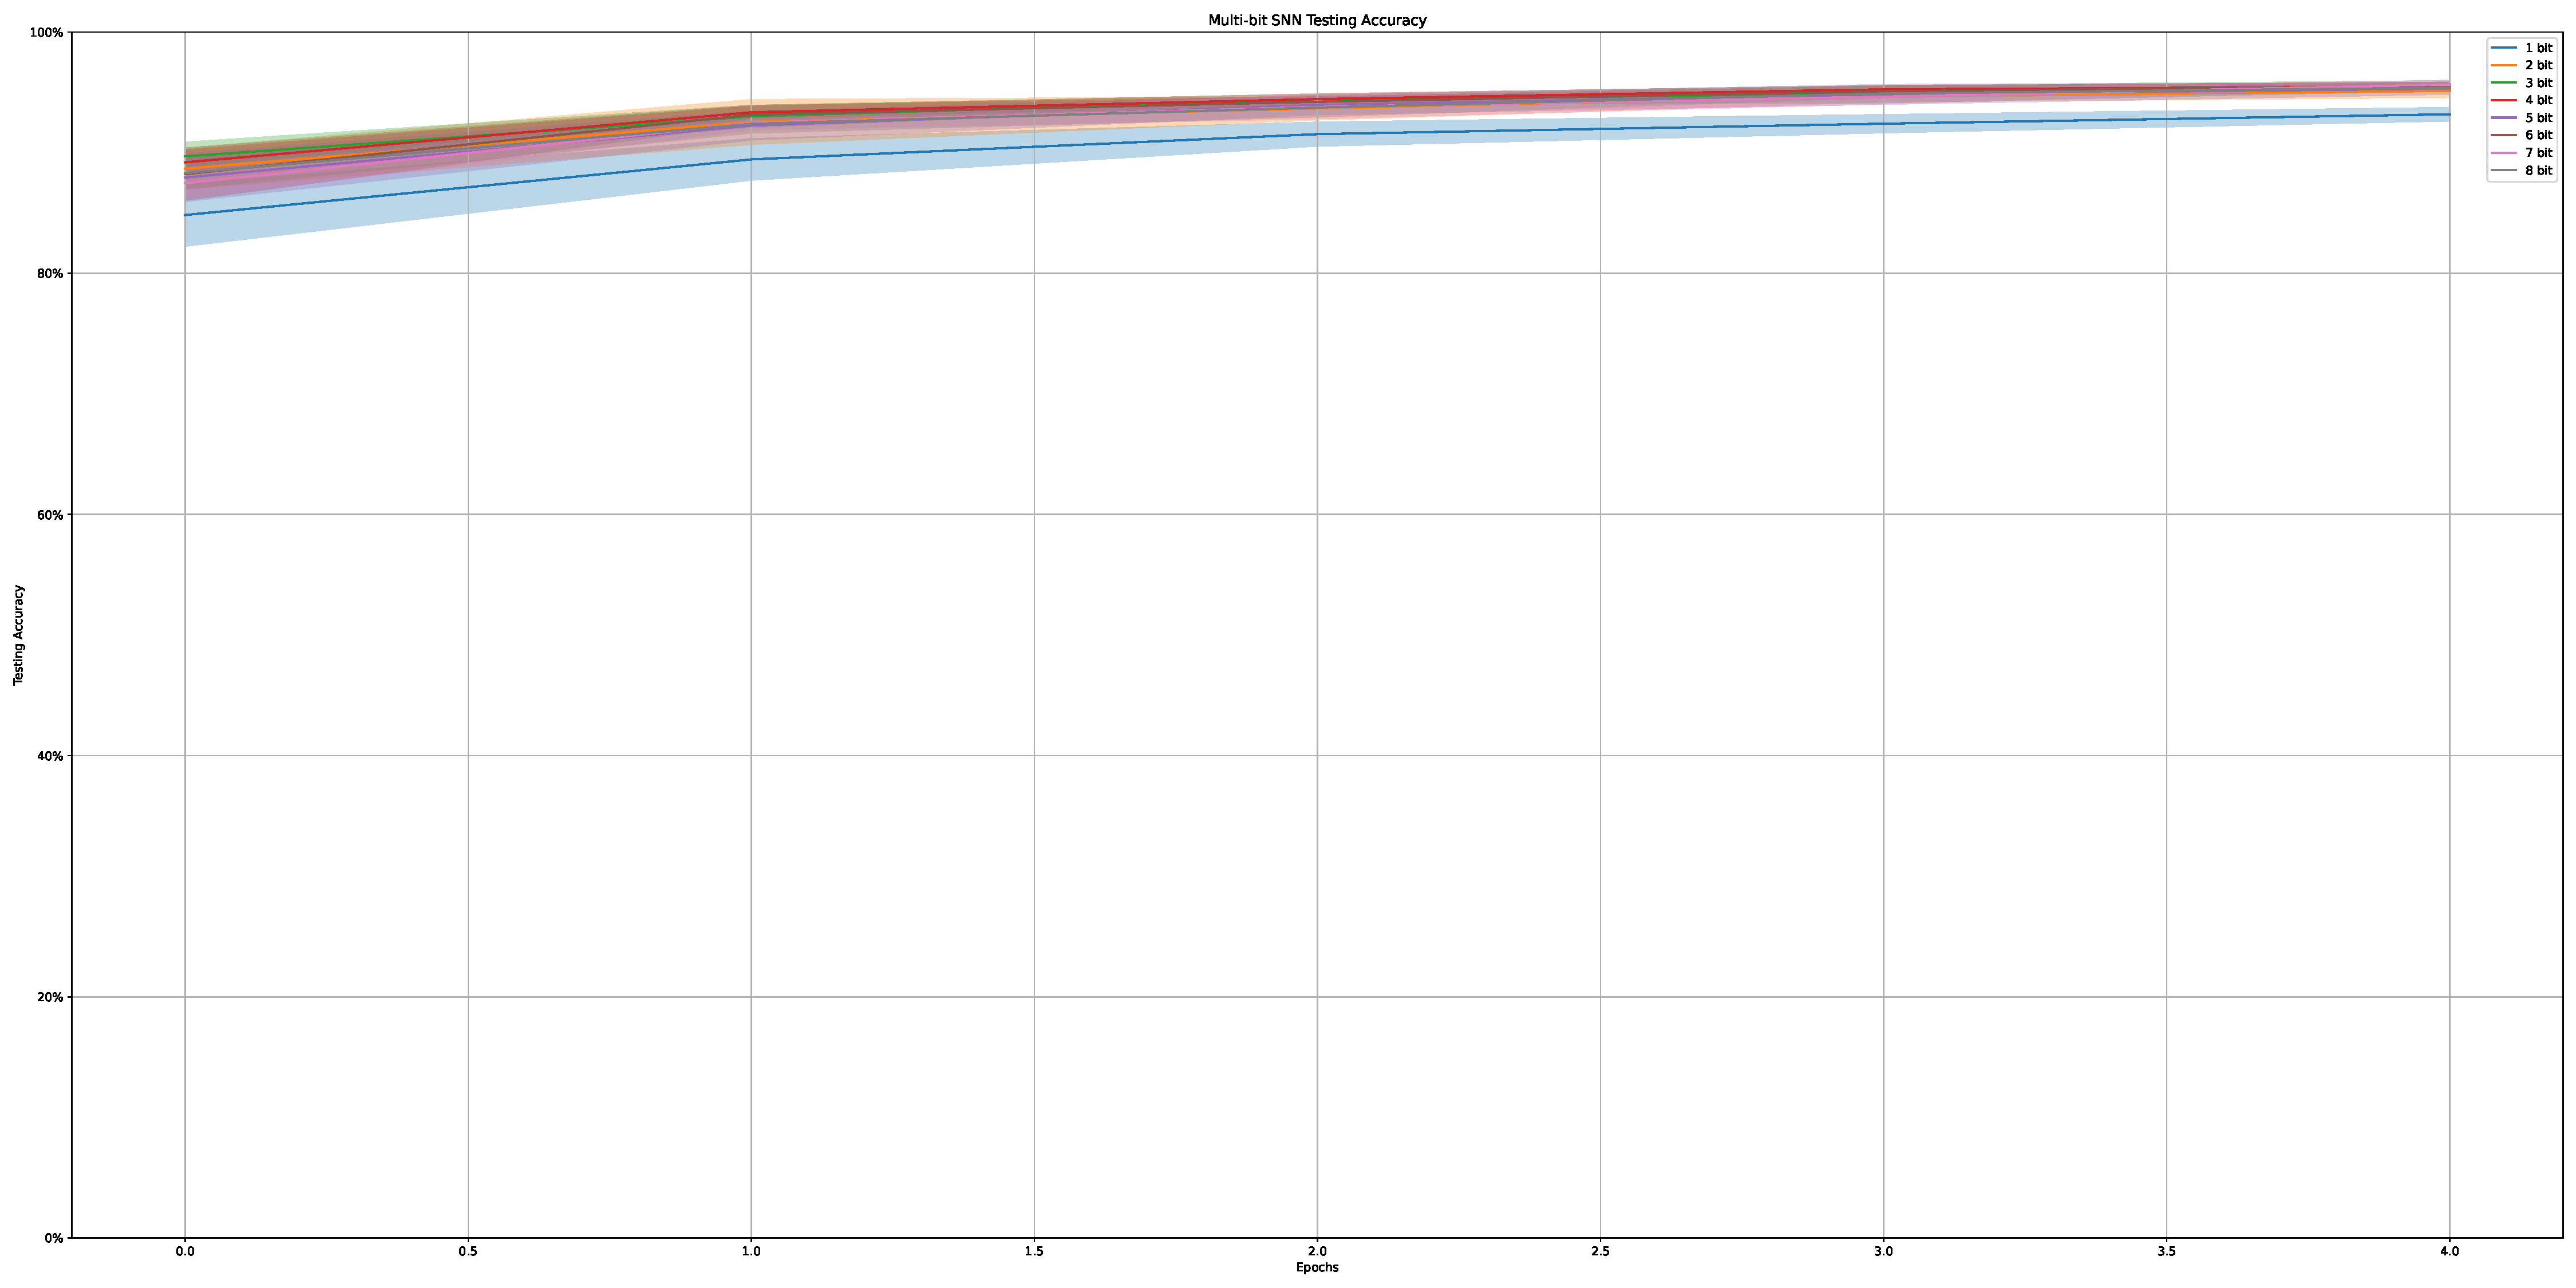
\includegraphics[width=\textwidth]{../standard/NMNIST/plots/nmnist_test_acc.pdf}
        %             \caption{Test Accuracy}
        %         \end{subfigure}
        %     \end{subfigure}
        %     \hfill
        %     \begin{subfigure}[H]{0.3\textwidth}
        %         \centering
        %         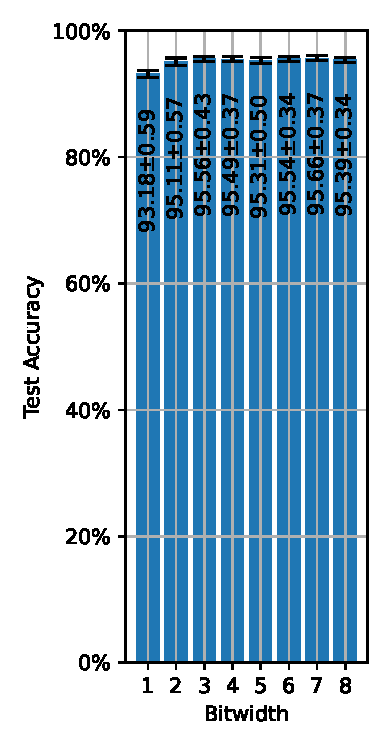
\includegraphics[width=\textwidth]{../standard/NMNIST/plots/nmnist_final_acc.pdf}
        %         \caption{Final Test Accuracy}
        %     \end{subfigure}
        %     \caption{Accuracy Curves of the NMNIST Model}
        % \end{figure}
        \begin{figure}[H]
            \centering
            \begin{subfigure}[H]{\textwidth}
                \centering
                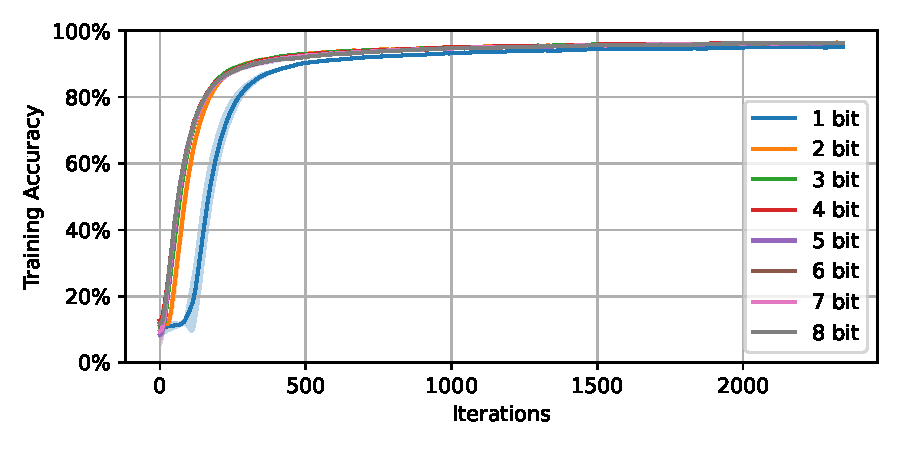
\includegraphics[width=\textwidth]{../standard/NMNIST/plots/nmnist_train_acc.pdf}
                \caption{Train Accuracy}
            \end{subfigure}
        \end{figure}
        \begin{figure}[H]
            \centering
            \ContinuedFloat
            \begin{subfigure}[H]{\textwidth}
                \centering
                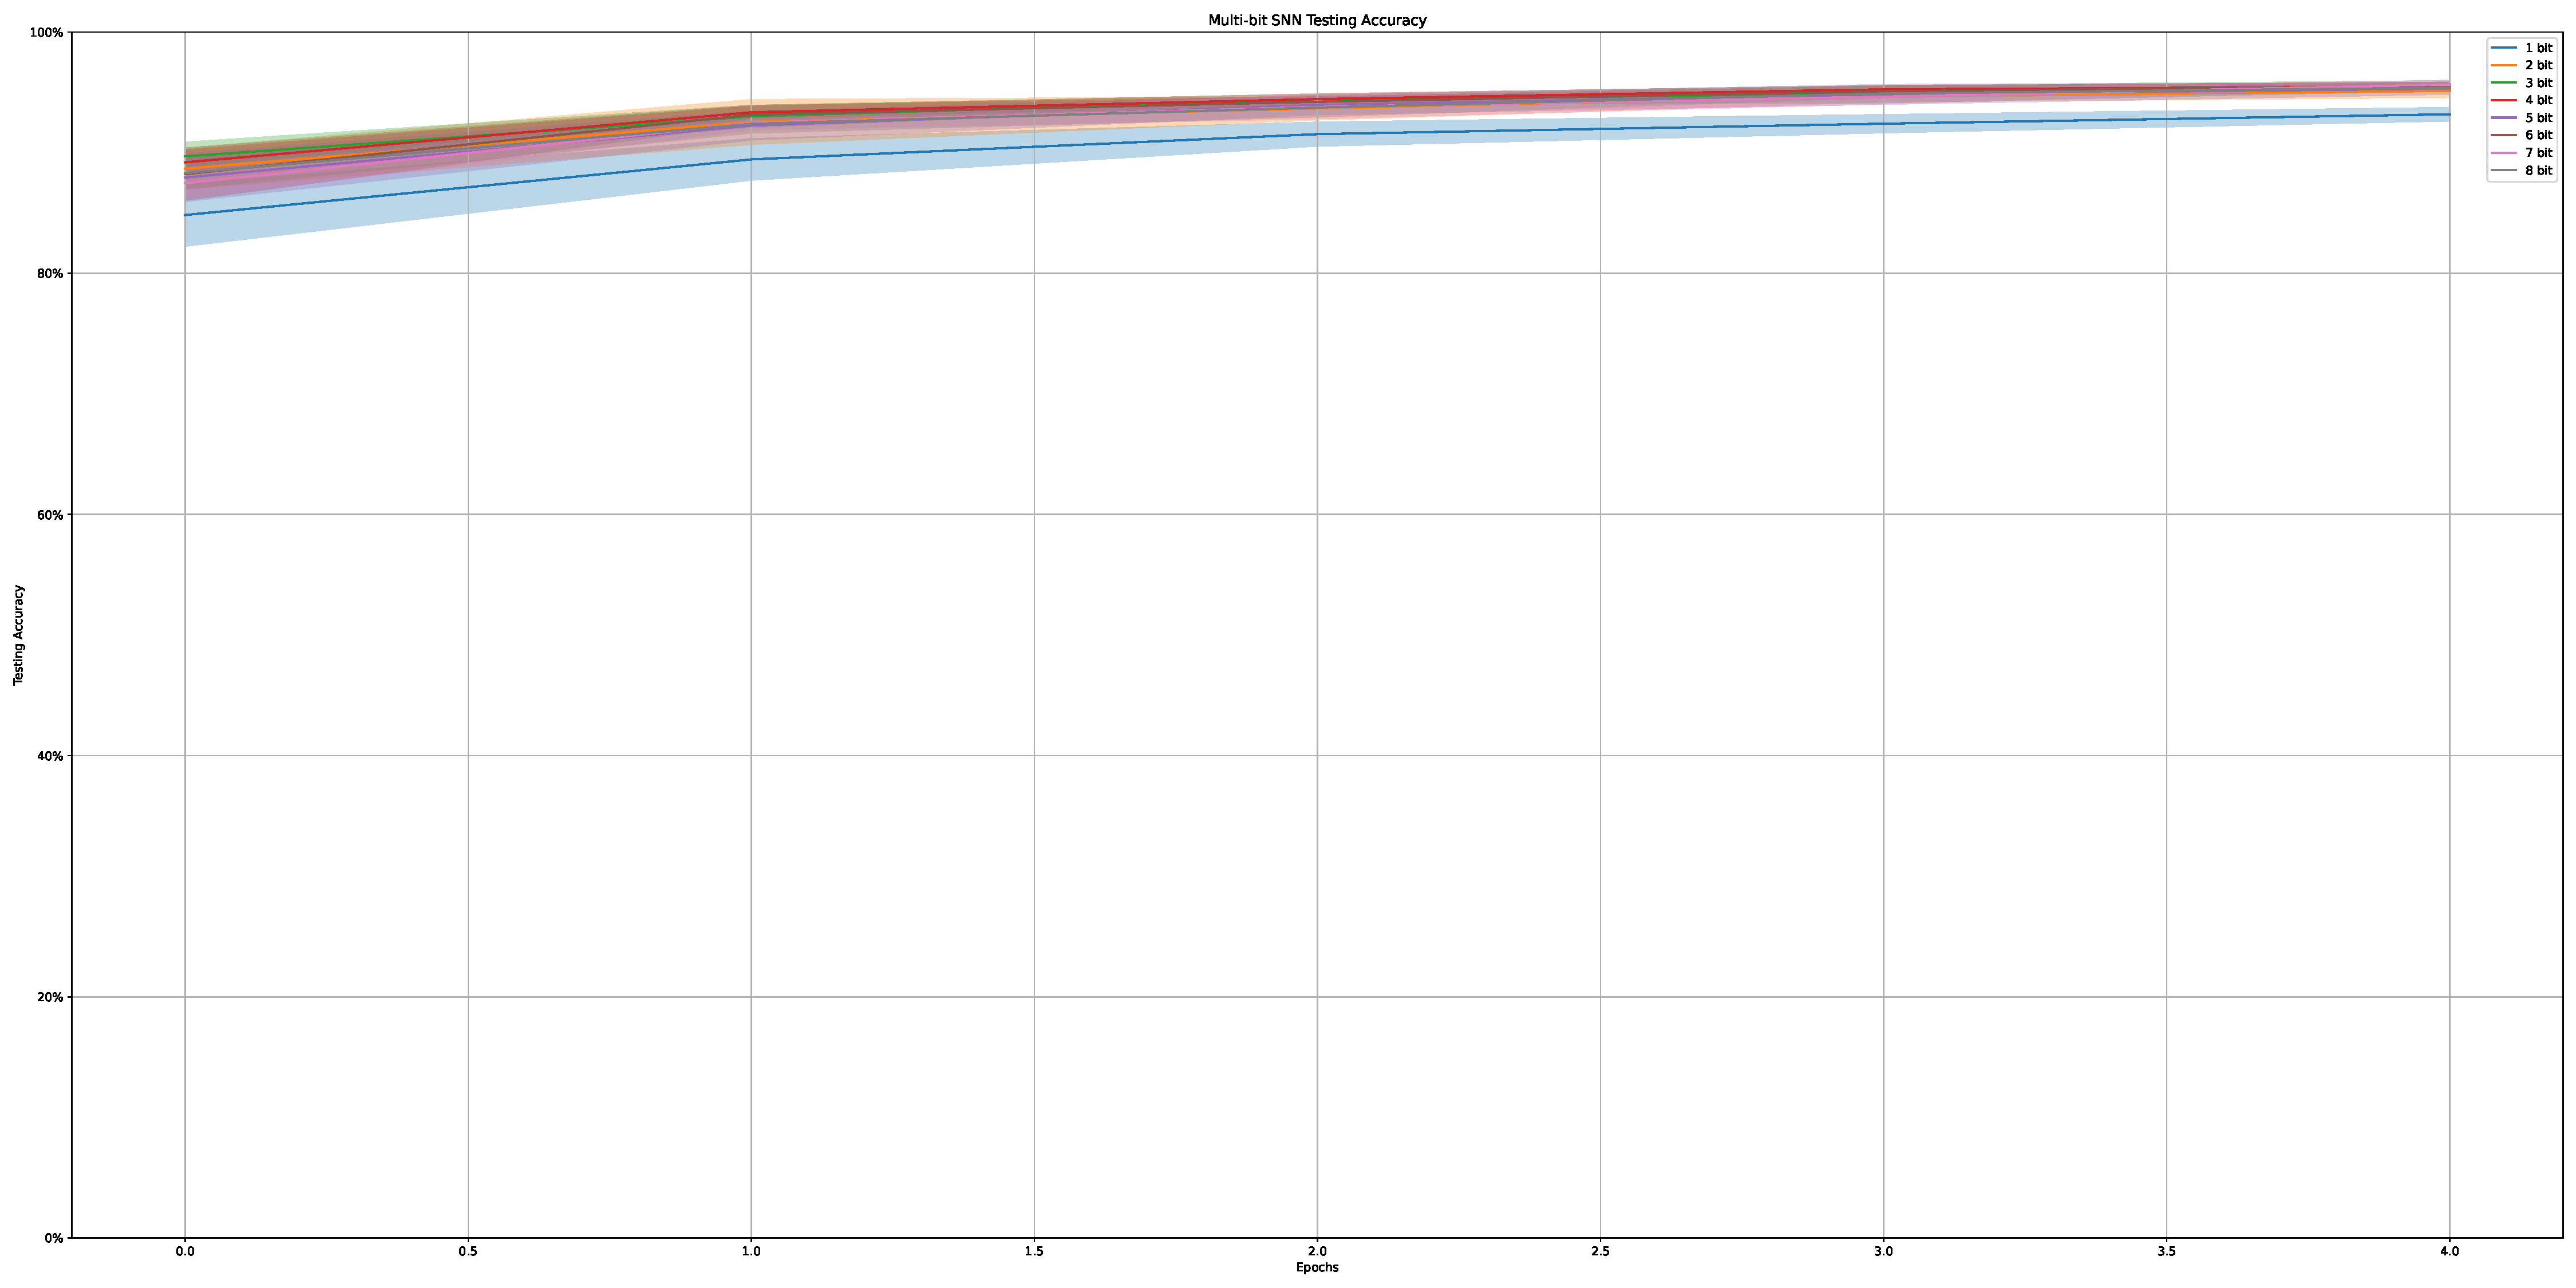
\includegraphics[width=\textwidth]{../standard/NMNIST/plots/nmnist_test_acc.pdf}
                \caption{Test Accuracy}
            \end{subfigure}
        \end{figure}
        \begin{figure}[H]
            \centering
            \ContinuedFloat
            \begin{subfigure}[H]{\textwidth}
                \centering
                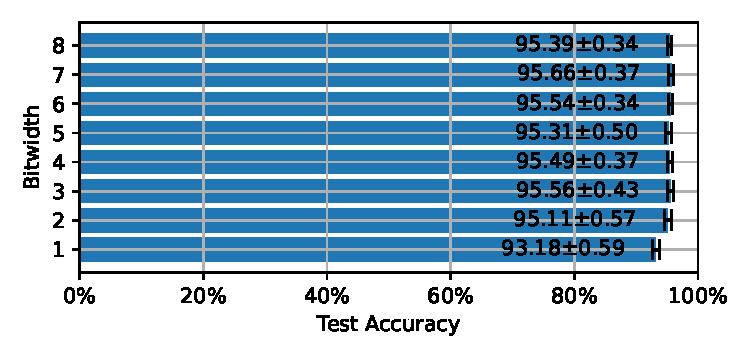
\includegraphics[width=\textwidth]{../standard/NMNIST/plots/nmnist_final_acc_horizontal.pdf}
                \caption{Final Test Accuracy}
            \end{subfigure}
            \caption{Accuracy Curves of the NMNIST Model}
        \end{figure}

    \label{appendix:accuracy_curves_dvs_gesture}
        % \begin{figure}[H]
        %     \centering
        %     \begin{subfigure}[H]{0.55\textwidth}
        %         \centering
        %         \begin{subfigure}[H]{\textwidth}
        %             \centering
        %             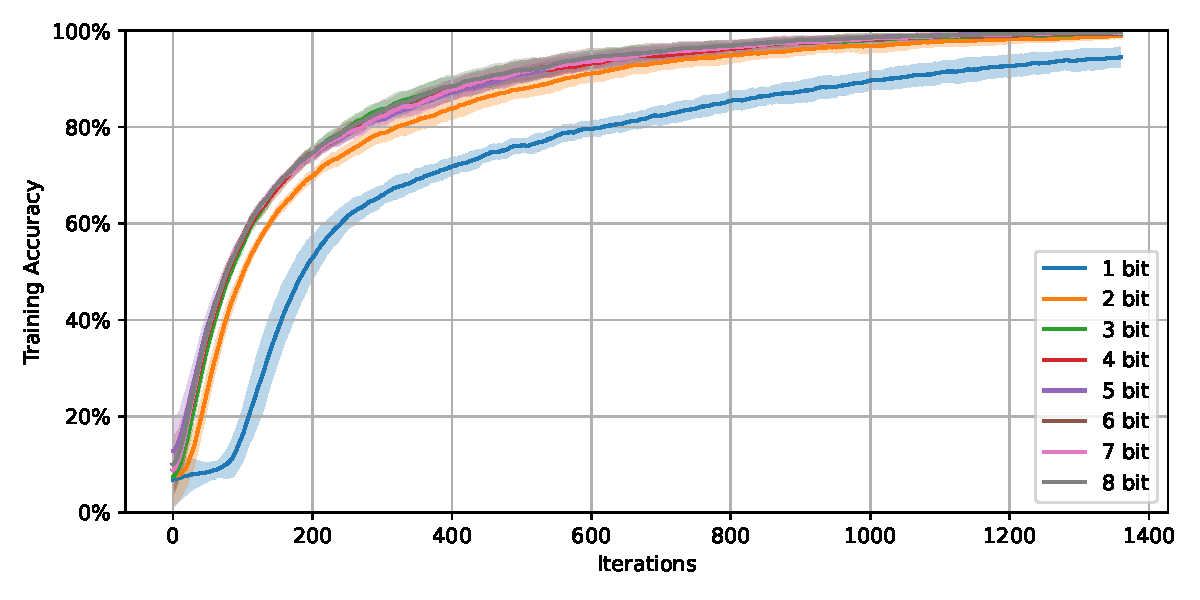
\includegraphics[width=\textwidth]{../standard/DVSGesture/plots/dvsgesture_train_acc.pdf}
        %             \caption{Train Accuracy}
        %         \end{subfigure}
        %         \hfill
        %         \begin{subfigure}[H]{\textwidth}
        %             \centering
        %             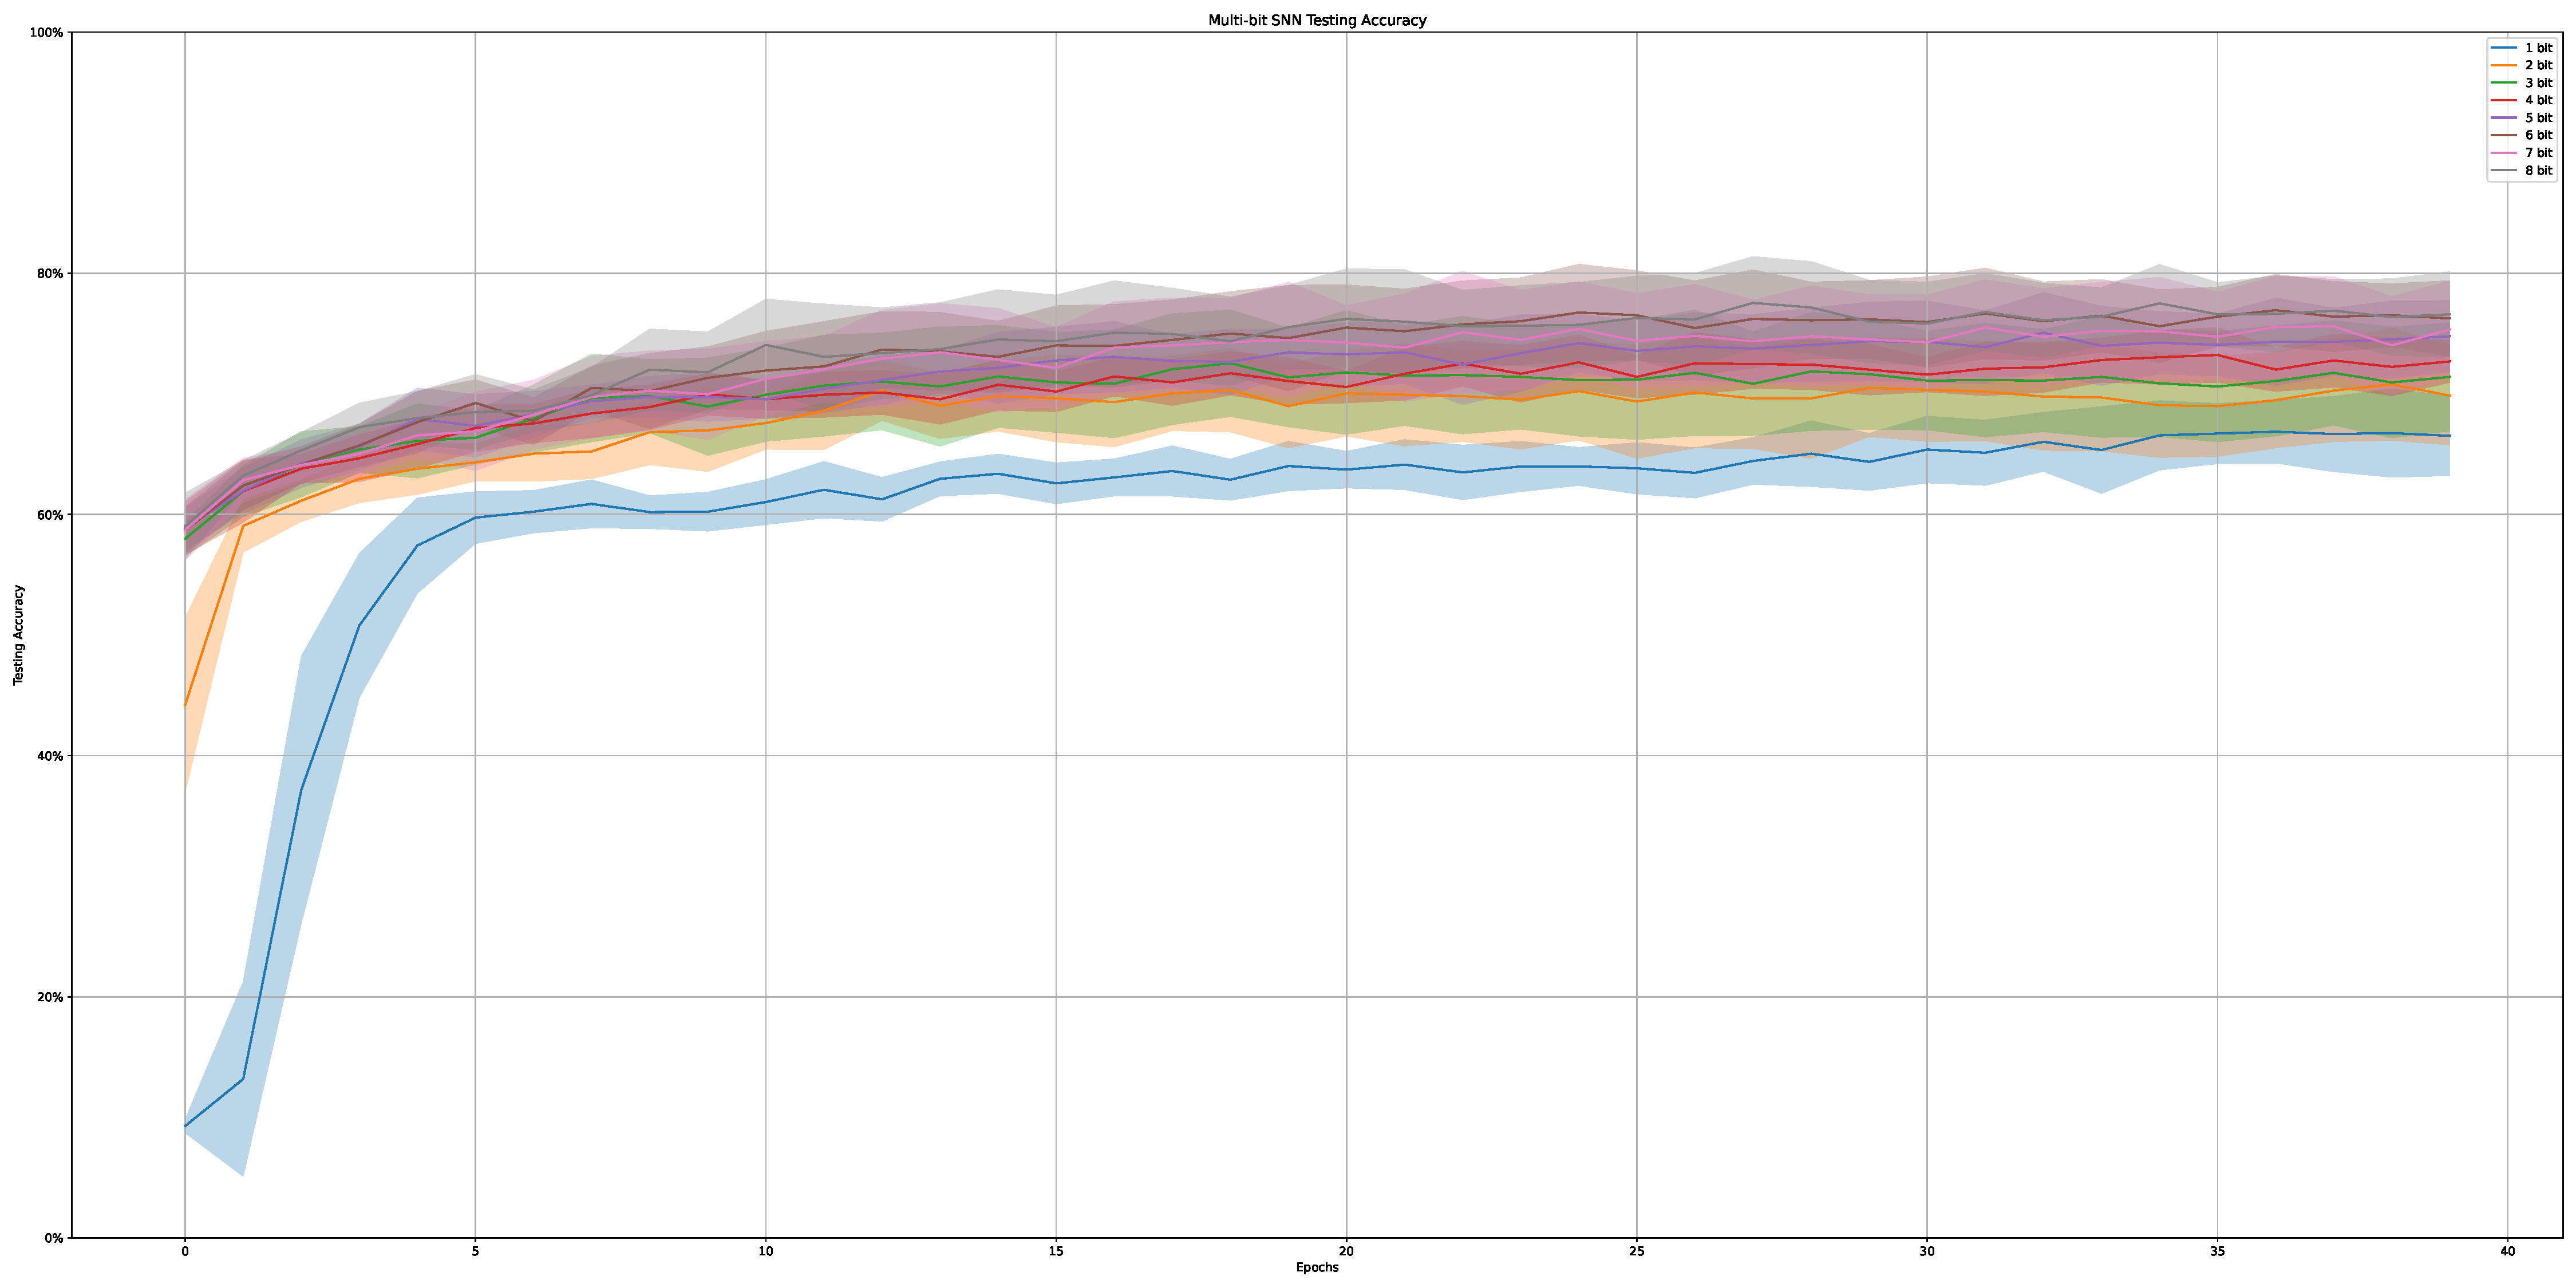
\includegraphics[width=\textwidth]{../standard/DVSGesture/plots/dvsgesture_test_acc.pdf}
        %             \caption{Test Accuracy}
        %         \end{subfigure}
        %     \end{subfigure}
        %     \hfill
        %     \begin{subfigure}[H]{0.3\textwidth}
        %         \centering
        %         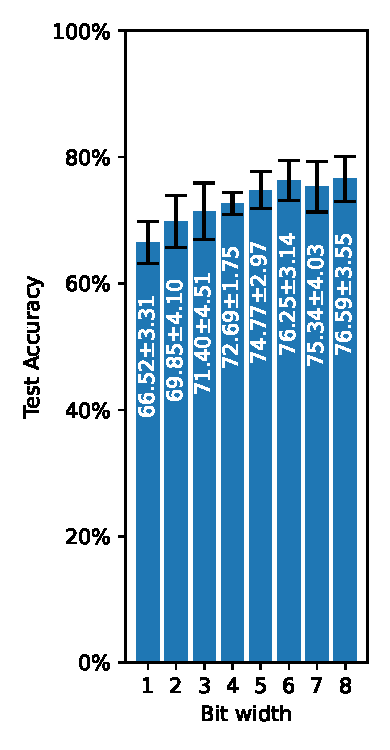
\includegraphics[width=\textwidth]{../standard/DVSGesture/plots/dvsgesture_final_acc.pdf}
        %         \caption{Final Test Accuracy}
        %     \end{subfigure}
        %     \caption{Accuracy Curves of the DVS Gesture Model}
        % \end{figure}
        \begin{figure}[H]
            \centering
            \begin{subfigure}[H]{\textwidth}
                \centering
                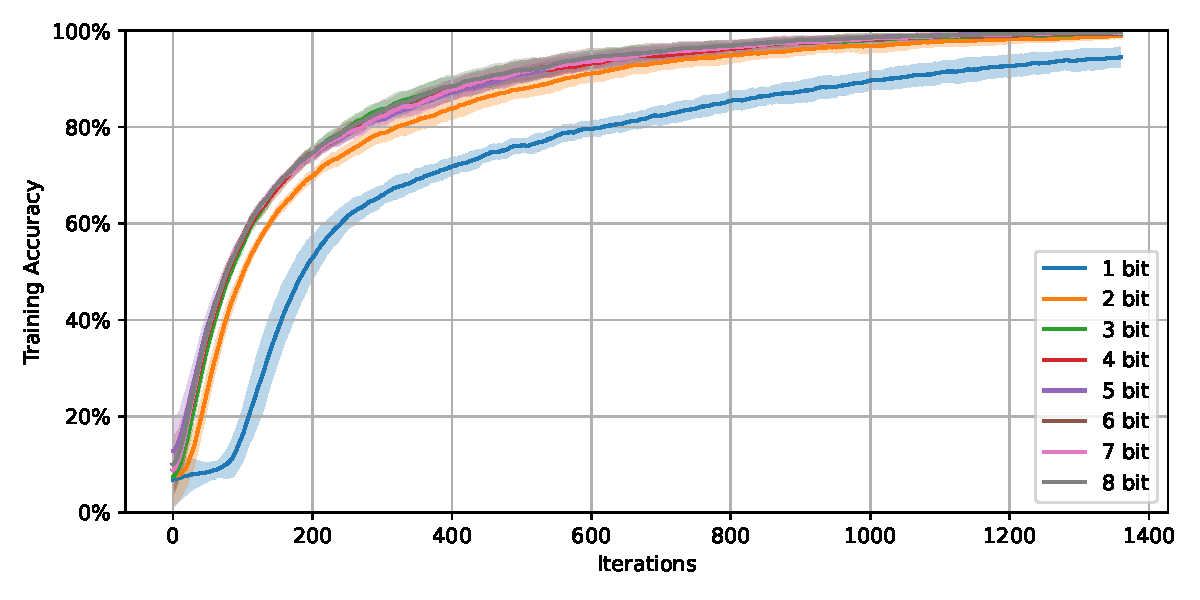
\includegraphics[width=\textwidth]{../standard/DVSGesture/plots/dvsgesture_train_acc.pdf}
                \caption{Train Accuracy}
            \end{subfigure}
        \end{figure}
        \begin{figure}[H]
            \centering
            \ContinuedFloat
            \begin{subfigure}[H]{\textwidth}
                \centering
                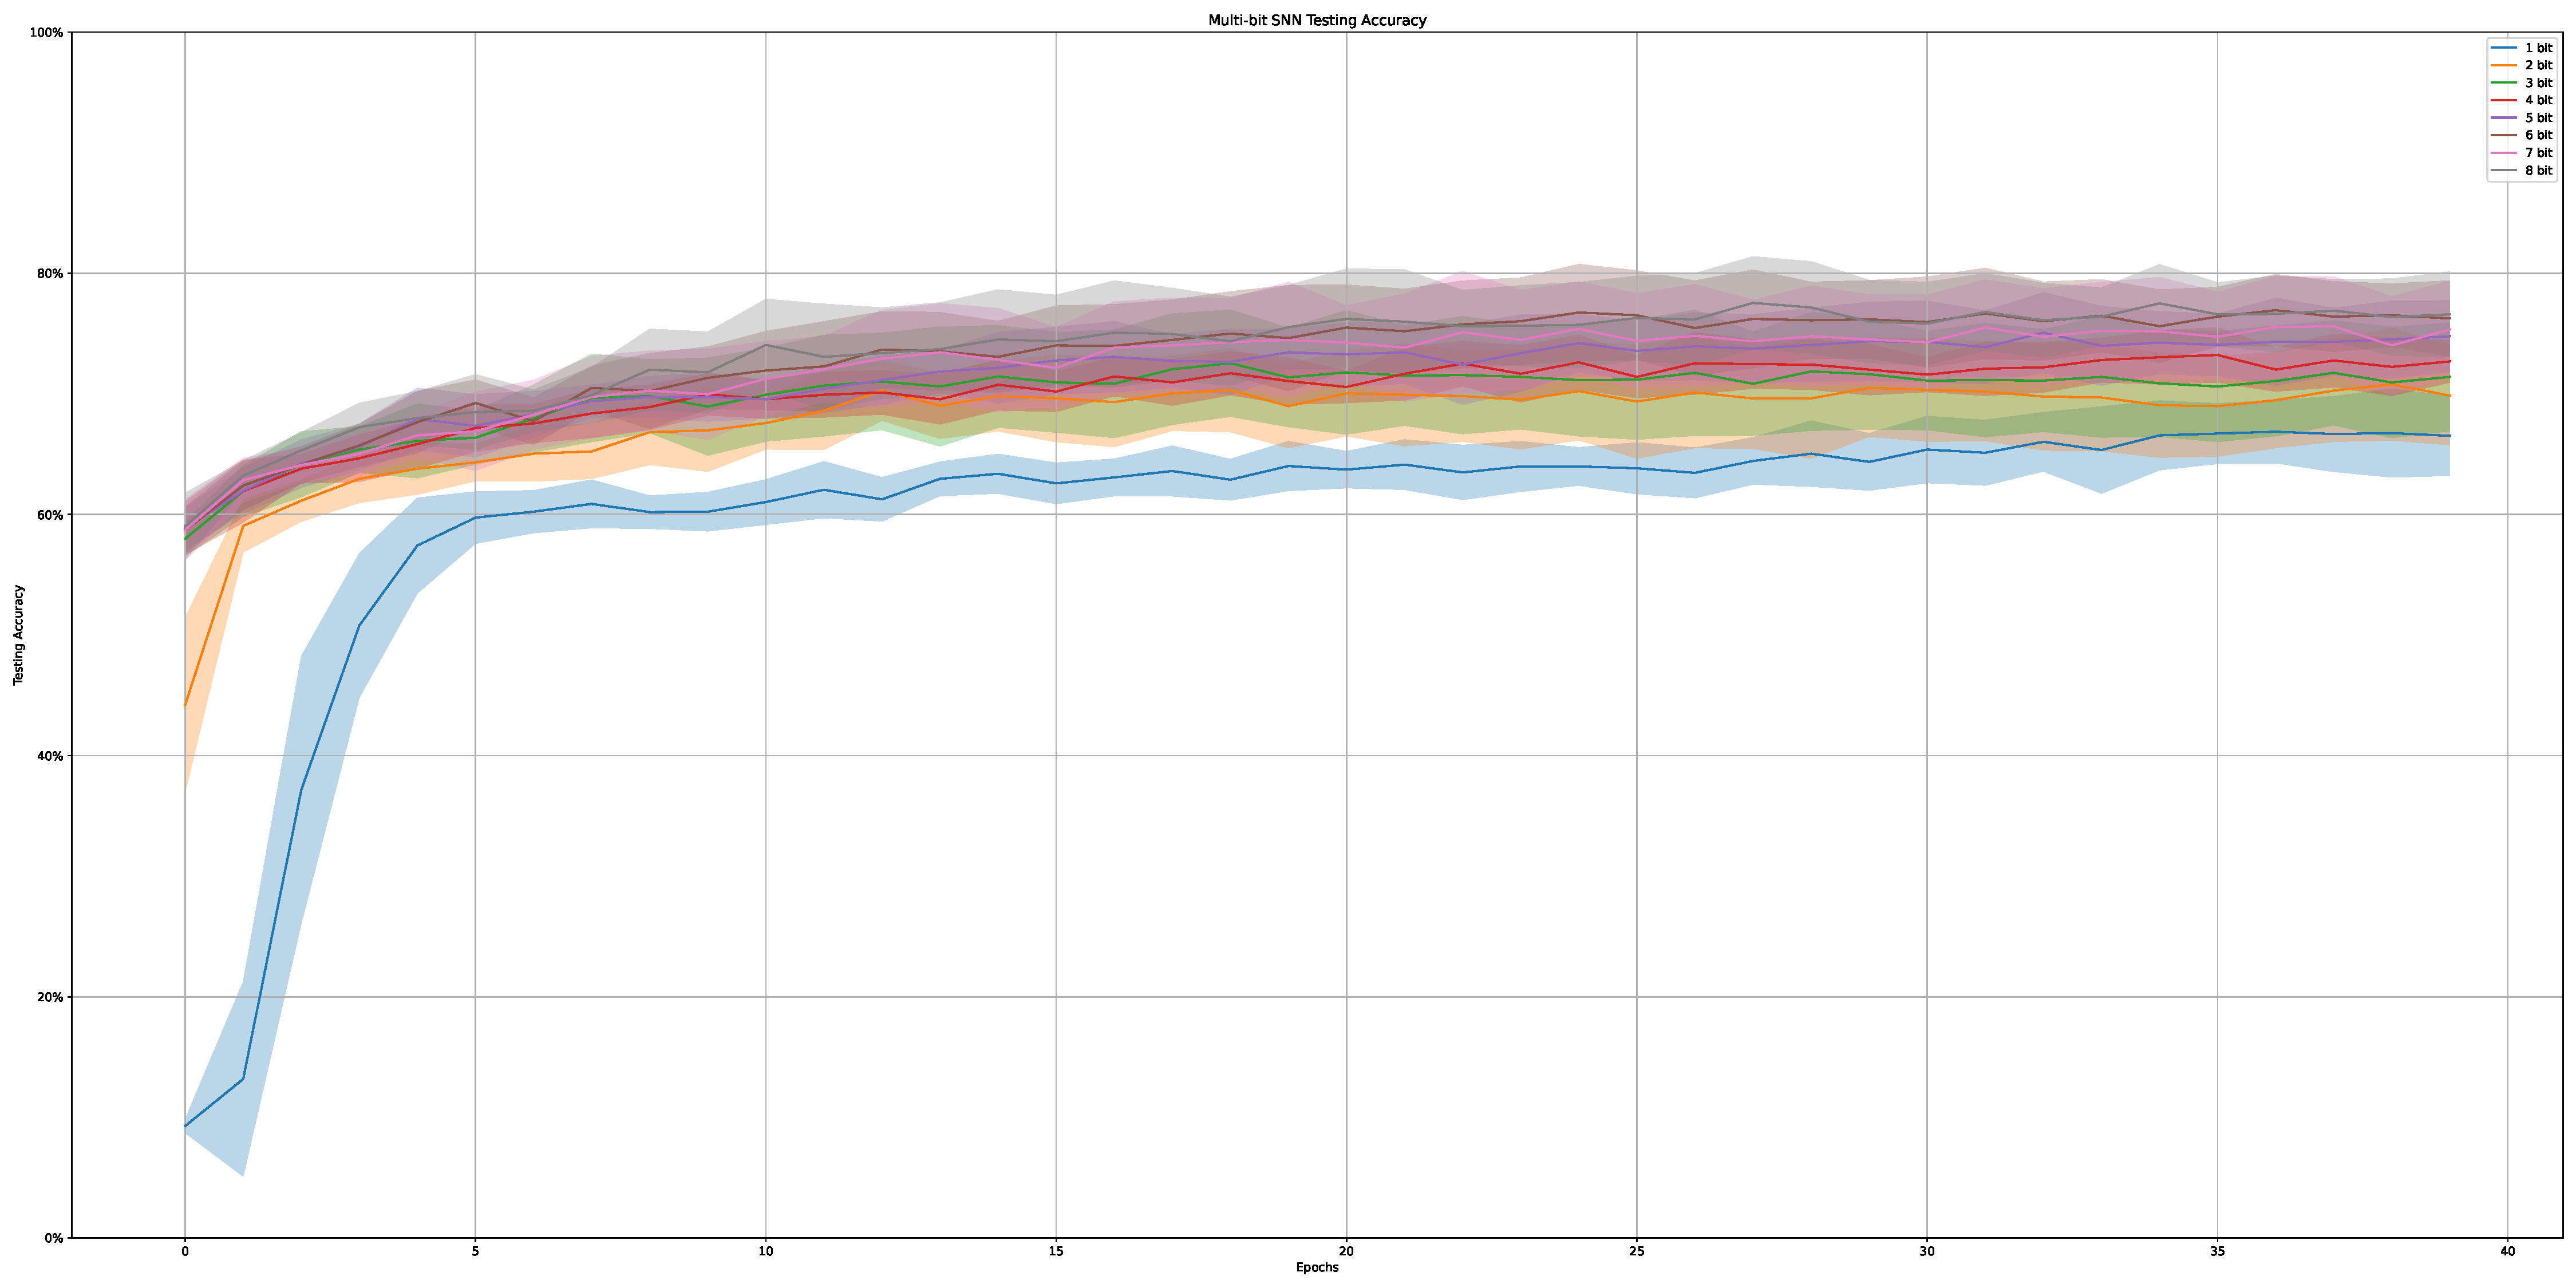
\includegraphics[width=\textwidth]{../standard/DVSGesture/plots/dvsgesture_test_acc.pdf}
                \caption{Test Accuracy}
            \end{subfigure}
        \end{figure}
        \begin{figure}[H]
            \centering
            \ContinuedFloat
            \begin{subfigure}[H]{\textwidth}
                \centering
                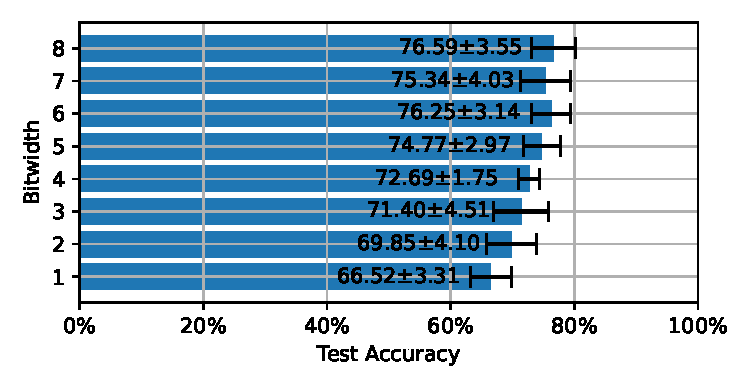
\includegraphics[width=\textwidth]{../standard/DVSGesture/plots/dvsgesture_final_acc_horizontal.pdf}
                \caption{Final Test Accuracy}
            \end{subfigure}
            \caption{Accuracy Curves of the DVS Gesture Model}
        \end{figure}

    \label{appendix:accuracy_curves_cifar10}
        % \begin{figure}[H]
        %     \centering
        %     \begin{subfigure}[H]{0.55\textwidth}
        %         \centering
        %         \begin{subfigure}[H]{\textwidth}
        %             \centering
        %             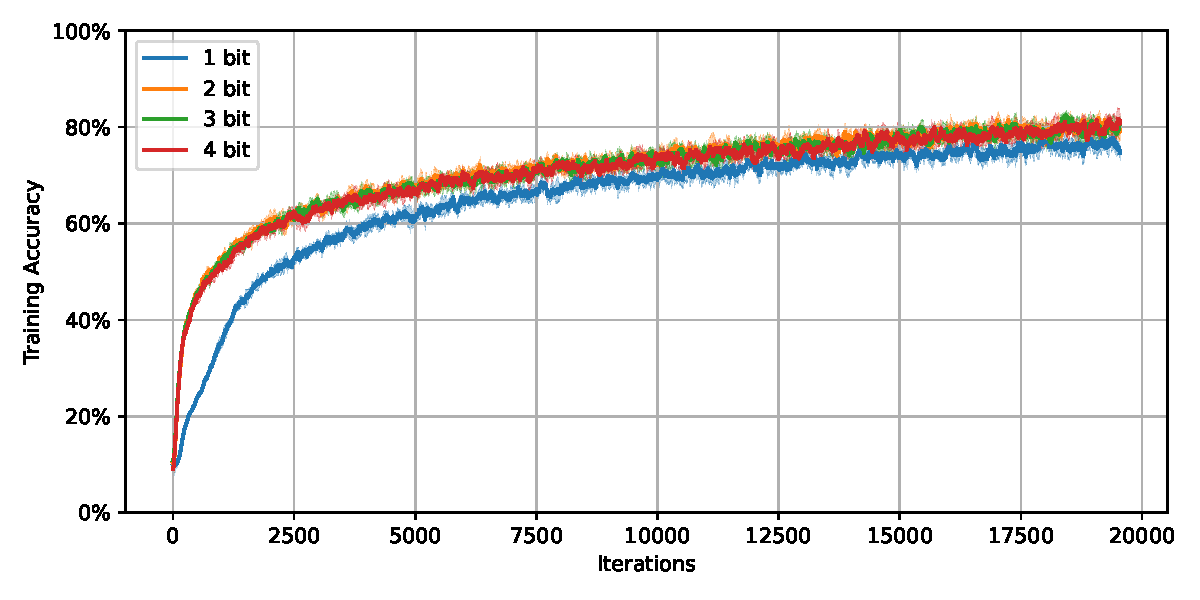
\includegraphics[width=\textwidth]{../standard/CIFAR10/plots/cifar10_train_acc.pdf}
        %             \caption{Train Accuracy}
        %         \end{subfigure}
        %         \hfill
        %         \begin{subfigure}[H]{\textwidth}
        %             \centering
        %             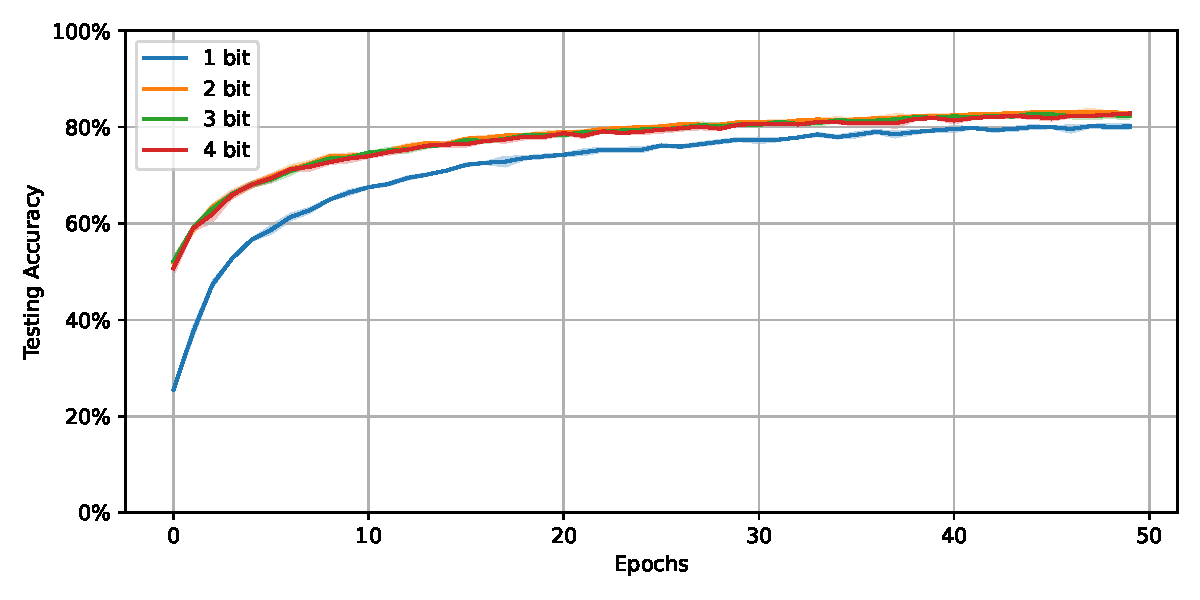
\includegraphics[width=\textwidth]{../standard/CIFAR10/plots/cifar10_test_acc.pdf}
        %             \caption{Test Accuracy}
        %         \end{subfigure}
        %     \end{subfigure}
        %     \hfill
        %     \begin{subfigure}[H]{0.3\textwidth}
        %         \centering
        %         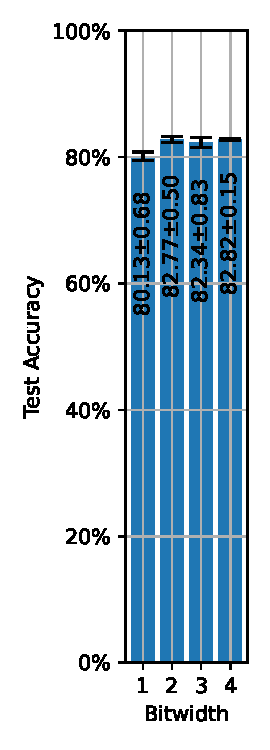
\includegraphics[width=\textwidth]{../standard/CIFAR10/plots/cifar10_final_acc.pdf}
        %         \caption{Final Test Accuracy}
        %     \end{subfigure}
        %     \caption{Accuracy Curves of the CIFAR-10 Model}
        % \end{figure}
        \begin{figure}[H]
            \centering
            \begin{subfigure}[H]{\textwidth}
                \centering
                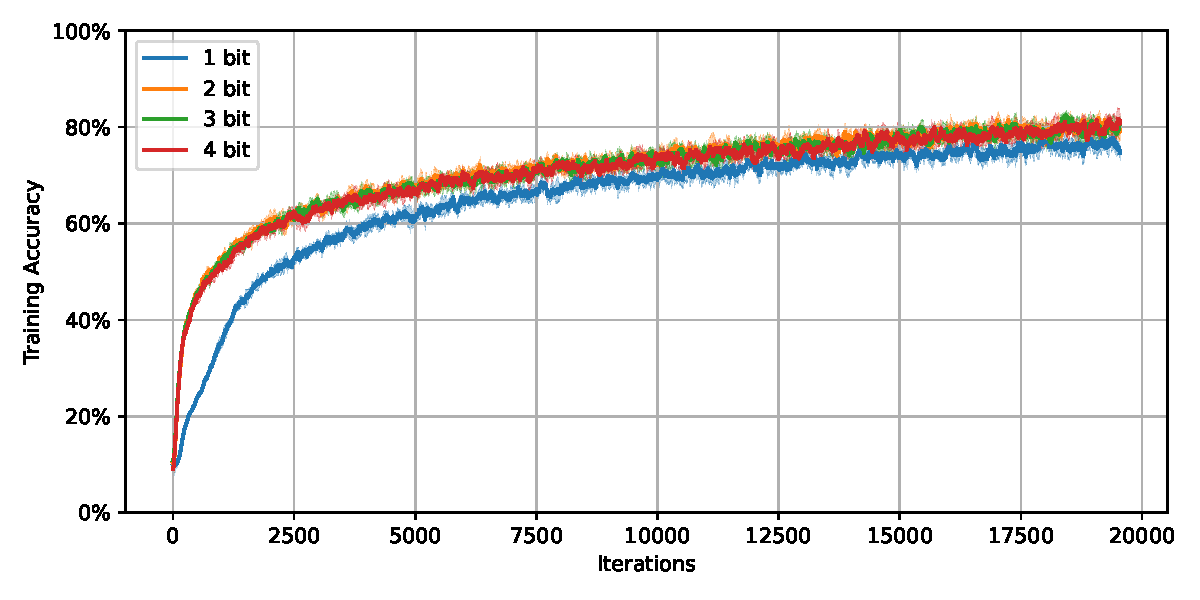
\includegraphics[width=\textwidth]{../standard/CIFAR10/plots/cifar10_train_acc.pdf}
                \caption{Train Accuracy}
            \end{subfigure}
        \end{figure}
        \begin{figure}[H]
            \centering
            \ContinuedFloat
            \begin{subfigure}[H]{\textwidth}
                \centering
                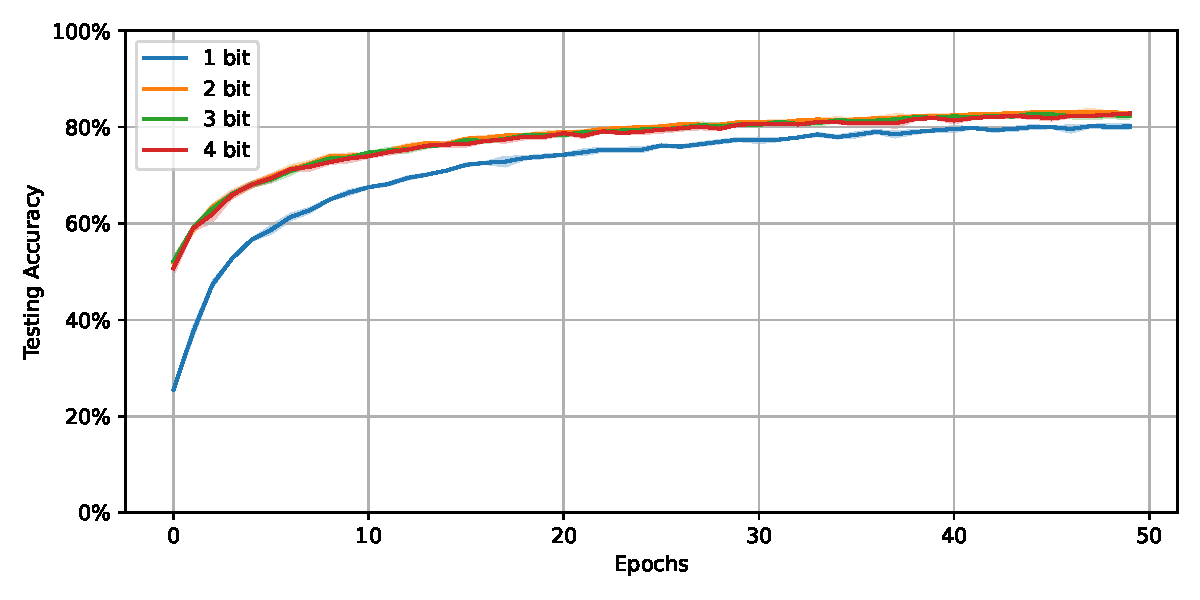
\includegraphics[width=\textwidth]{../standard/CIFAR10/plots/cifar10_test_acc.pdf}
                \caption{Test Accuracy}
            \end{subfigure}
        \end{figure}
        \begin{figure}[H]
            \centering
            \ContinuedFloat
            \begin{subfigure}[H]{\textwidth}
                \centering
                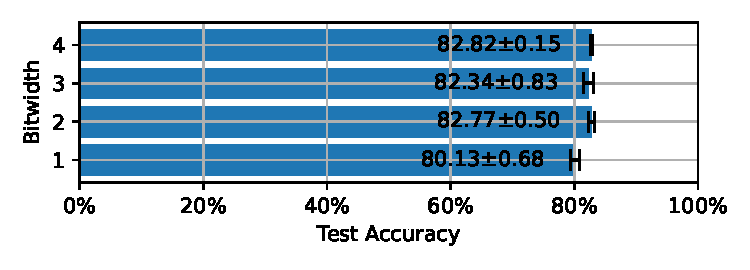
\includegraphics[width=\textwidth]{../standard/CIFAR10/plots/cifar10_final_acc_horizontal.pdf}
                \caption{Final Test Accuracy}
            \end{subfigure}
            \caption{Accuracy Curves of the CIFAR-10 Model}
        \end{figure}

\section{Iterations and Epochs to Reach the Target Accuracy}
\label{appendix:iterations}
    In this section, we consider the target accuracy to be 80\%. 

    Hyperparameters: Same as in Table \ref{tab:hyperparameters_accuracy}.

    \label{appendix:iterations_fashion_mnist}
        \begin{figure}[H]
            \centering
            \begin{subfigure}[H]{\textwidth}
                \centering
                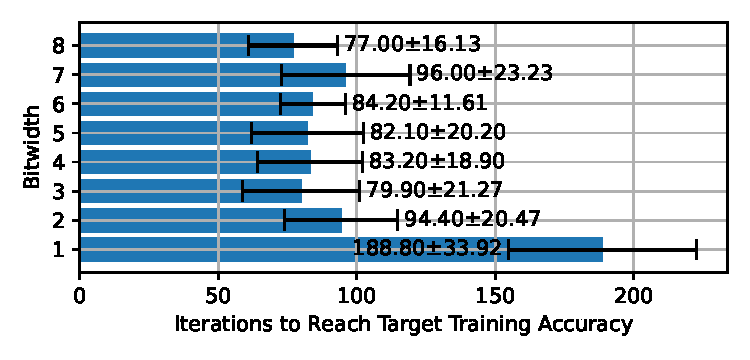
\includegraphics[width=\textwidth]{../standard/FashionMNIST/plots/fashionmnist_train_iters_horizontal.pdf}
                \caption{Iterations to Reach the Training Accuracy}
            \end{subfigure}
        \end{figure}
        \begin{figure}[H]
            \centering
            \ContinuedFloat
            \begin{subfigure}[H]{\textwidth}
                \centering
                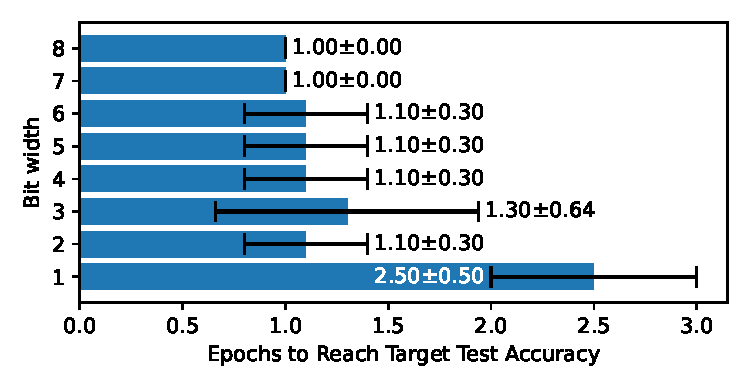
\includegraphics[width=\textwidth]{../standard/FashionMNIST/plots/fashionmnist_test_iters_horizontal.pdf}
                \caption{Epochs to Reach the Test Accuracy}
            \end{subfigure}
            \caption{Required Iterations of Epochs on Fashion MNIST}
        \end{figure}

    \label{appendix:iterations_mnist}
        \begin{figure}[H]
            \centering
            \begin{subfigure}[H]{\textwidth}
                \centering
                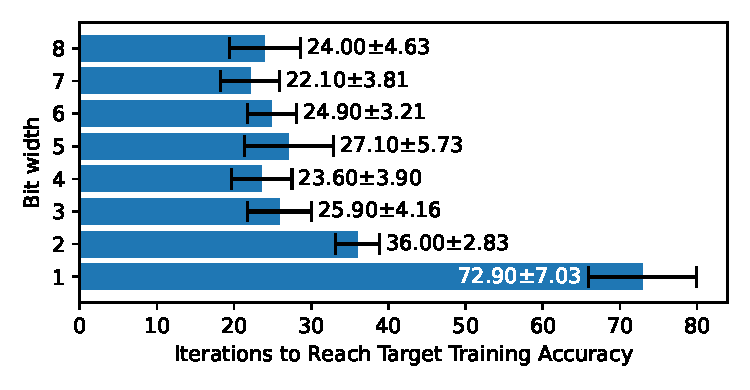
\includegraphics[width=\textwidth]{../standard/MNIST/plots/mnist_train_iters_horizontal.pdf}
                \caption{Iterations to Reach the Training Accuracy}
            \end{subfigure}
        \end{figure}
        \begin{figure}[H]
            \centering
            \ContinuedFloat
            \begin{subfigure}[H]{\textwidth}
                \centering
                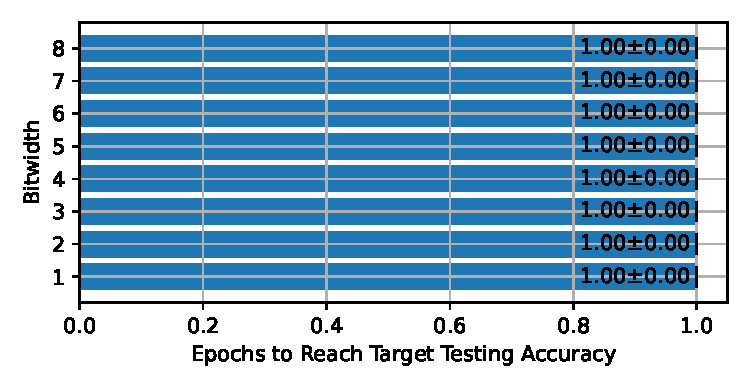
\includegraphics[width=\textwidth]{../standard/MNIST/plots/mnist_test_iters_horizontal.pdf}
                \caption{Epochs to Reach the Test Accuracy}
            \end{subfigure}
            \caption{Required Iterations of Epochs on MNIST}
        \end{figure}

    \label{appendix:iterations_nmnist}
        \begin{figure}[H]
            \centering
            \begin{subfigure}[H]{\textwidth}
                \centering
                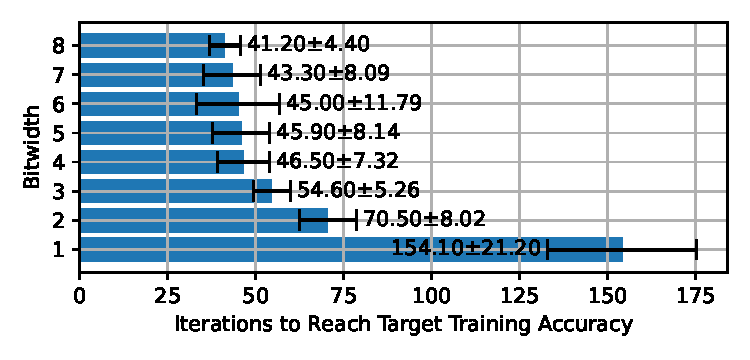
\includegraphics[width=\textwidth]{../standard/NMNIST/plots/nmnist_train_iters_horizontal.pdf}
                \caption{Iterations to Reach the Training Accuracy}
            \end{subfigure}
        \end{figure}
        \begin{figure}[H]
            \centering
            \ContinuedFloat
            \begin{subfigure}[H]{\textwidth}
                \centering
                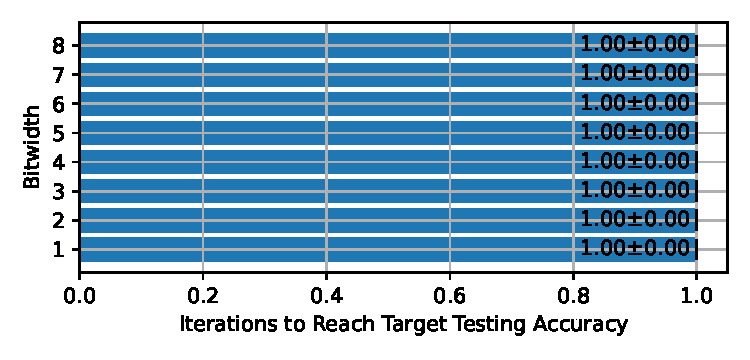
\includegraphics[width=\textwidth]{../standard/NMNIST/plots/nmnist_test_iters_horizontal.pdf}
                \caption{Epochs to Reach the Test Accuracy}
            \end{subfigure}
            \caption{Required Iterations of Epochs on NMNIST}
        \end{figure}

    \label{appendix:iterations_dvs_gesture}
        \begin{figure}[H]
            \centering
            \begin{subfigure}[H]{\textwidth}
                \centering
                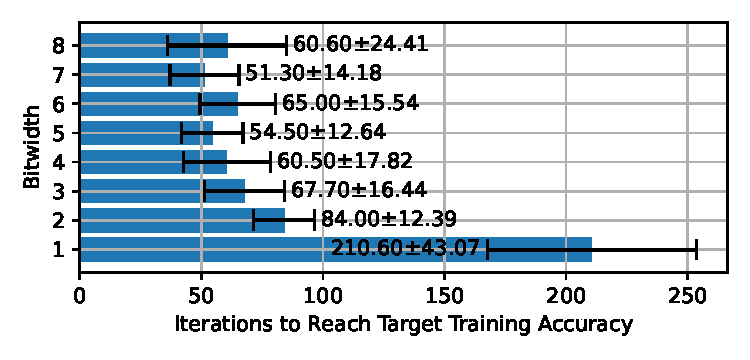
\includegraphics[width=\textwidth]{../standard/DVSGesture/plots/dvsgesture_train_iters_horizontal.pdf}
                \caption{Iterations to Reach the Training Accuracy}
            \end{subfigure}
        \end{figure}
        \begin{figure}[H]
            \centering
            \ContinuedFloat
            \begin{subfigure}[H]{\textwidth}
                \centering
                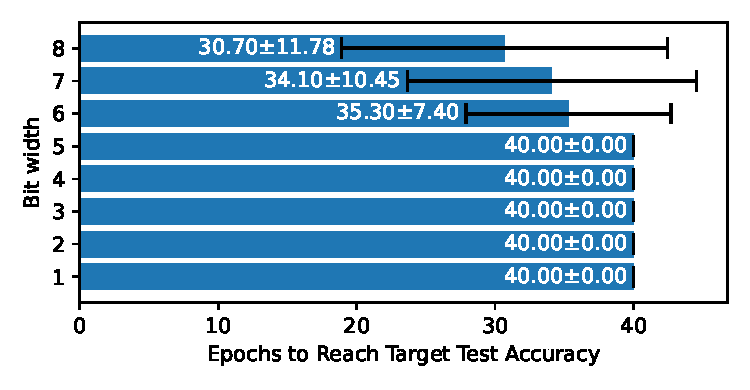
\includegraphics[width=\textwidth]{../standard/DVSGesture/plots/dvsgesture_test_iters_horizontal.pdf}
                \caption{Epochs to Reach the Test Accuracy}
            \end{subfigure}
            \caption{Required Iterations of Epochs on DVS Gesture}
        \end{figure}

    Notice that we encountered overfitting in the DVS Gesture dataset, which is why the number of iterations to reach the target test accuracy is capped at 40 epochs (the maximum number of epochs in the training process), thus not representative. 

    \label{appendix:iterations_cifar10}
        \begin{figure}[H]
            \centering
            \begin{subfigure}[H]{\textwidth}
                \centering
                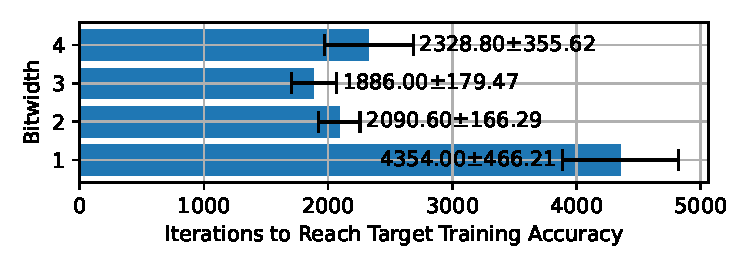
\includegraphics[width=\textwidth]{../standard/CIFAR10/plots/cifar10_train_iters_horizontal.pdf}
                \caption{Iterations to Reach the Training Accuracy}
            \end{subfigure}
        \end{figure}
        \begin{figure}[H]
            \centering
            \ContinuedFloat
            \begin{subfigure}[H]{\textwidth}
                \centering
                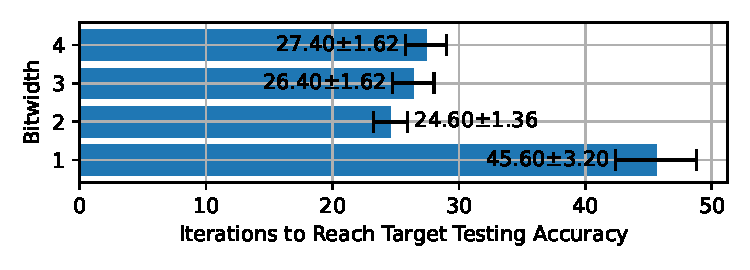
\includegraphics[width=\textwidth]{../standard/CIFAR10/plots/cifar10_test_iters_horizontal.pdf}
                \caption{Epochs to Reach the Test Accuracy}
            \end{subfigure}
            \caption{Required Iterations of Epochs on CIFAR-10}
        \end{figure}



\chapter{Firing Rate in Different Positions of the Multi-Bit Spike Train Model}
\label{appendix:firerate}

    For the ease of debugging, the first measuring position is always just the input data. If the data is captured by a dynamic vision sensor or it is encoded with a Poisson spike generator, one should see a firing rate much below 100\%. In the case of original data (e.g. CIFAR-10), the firing rate should be close to 100\%. 

    From the second measuring position to the last position, the firing rate is measured after the LIF neuron layers. Not all LIF neuron layers are measured. But the last LIF neuron layer is always measured. 

    The hyperparameters used in the training process are shown in Table \ref{tab:hyperparameters_firerate}.

    \begin{table}
        \begin{tabularx}{\textwidth}{|X|c|c|c|c|c|c|c|}
            \toprule
            Dataset & Reps & Epochs & LR & Opt & Batch & Time steps \\
            \midrule
            Fashion MNIST & 10 & 50 & 2e-3 & Adam & 128 & 10 \\
            MNIST & 10 & 50 & 2e-3 & Adam & 128 & 10 \\
            NMNIST & 10 & 50 & 2e-3 & Adam & 128 & 10 \\
            DVS Gesture & 10 & 200 & 1e-3 & Adam & 128 & 10 \\
            CIFAR-10 & 5 & 1000 & 1e-5 & Adam & 128 & 10 \\
            \bottomrule
        \end{tabularx}
        \caption{Hyperparameters}
        \label{tab:hyperparameters_firerate}
    \end{table}

    \section{Fashion MNIST}
    \label{appendix:firerate_fashion_mnist}
        \begin{figure}[H]
            \centering
            \begin{subfigure}[H]{\textwidth}
                \centering
                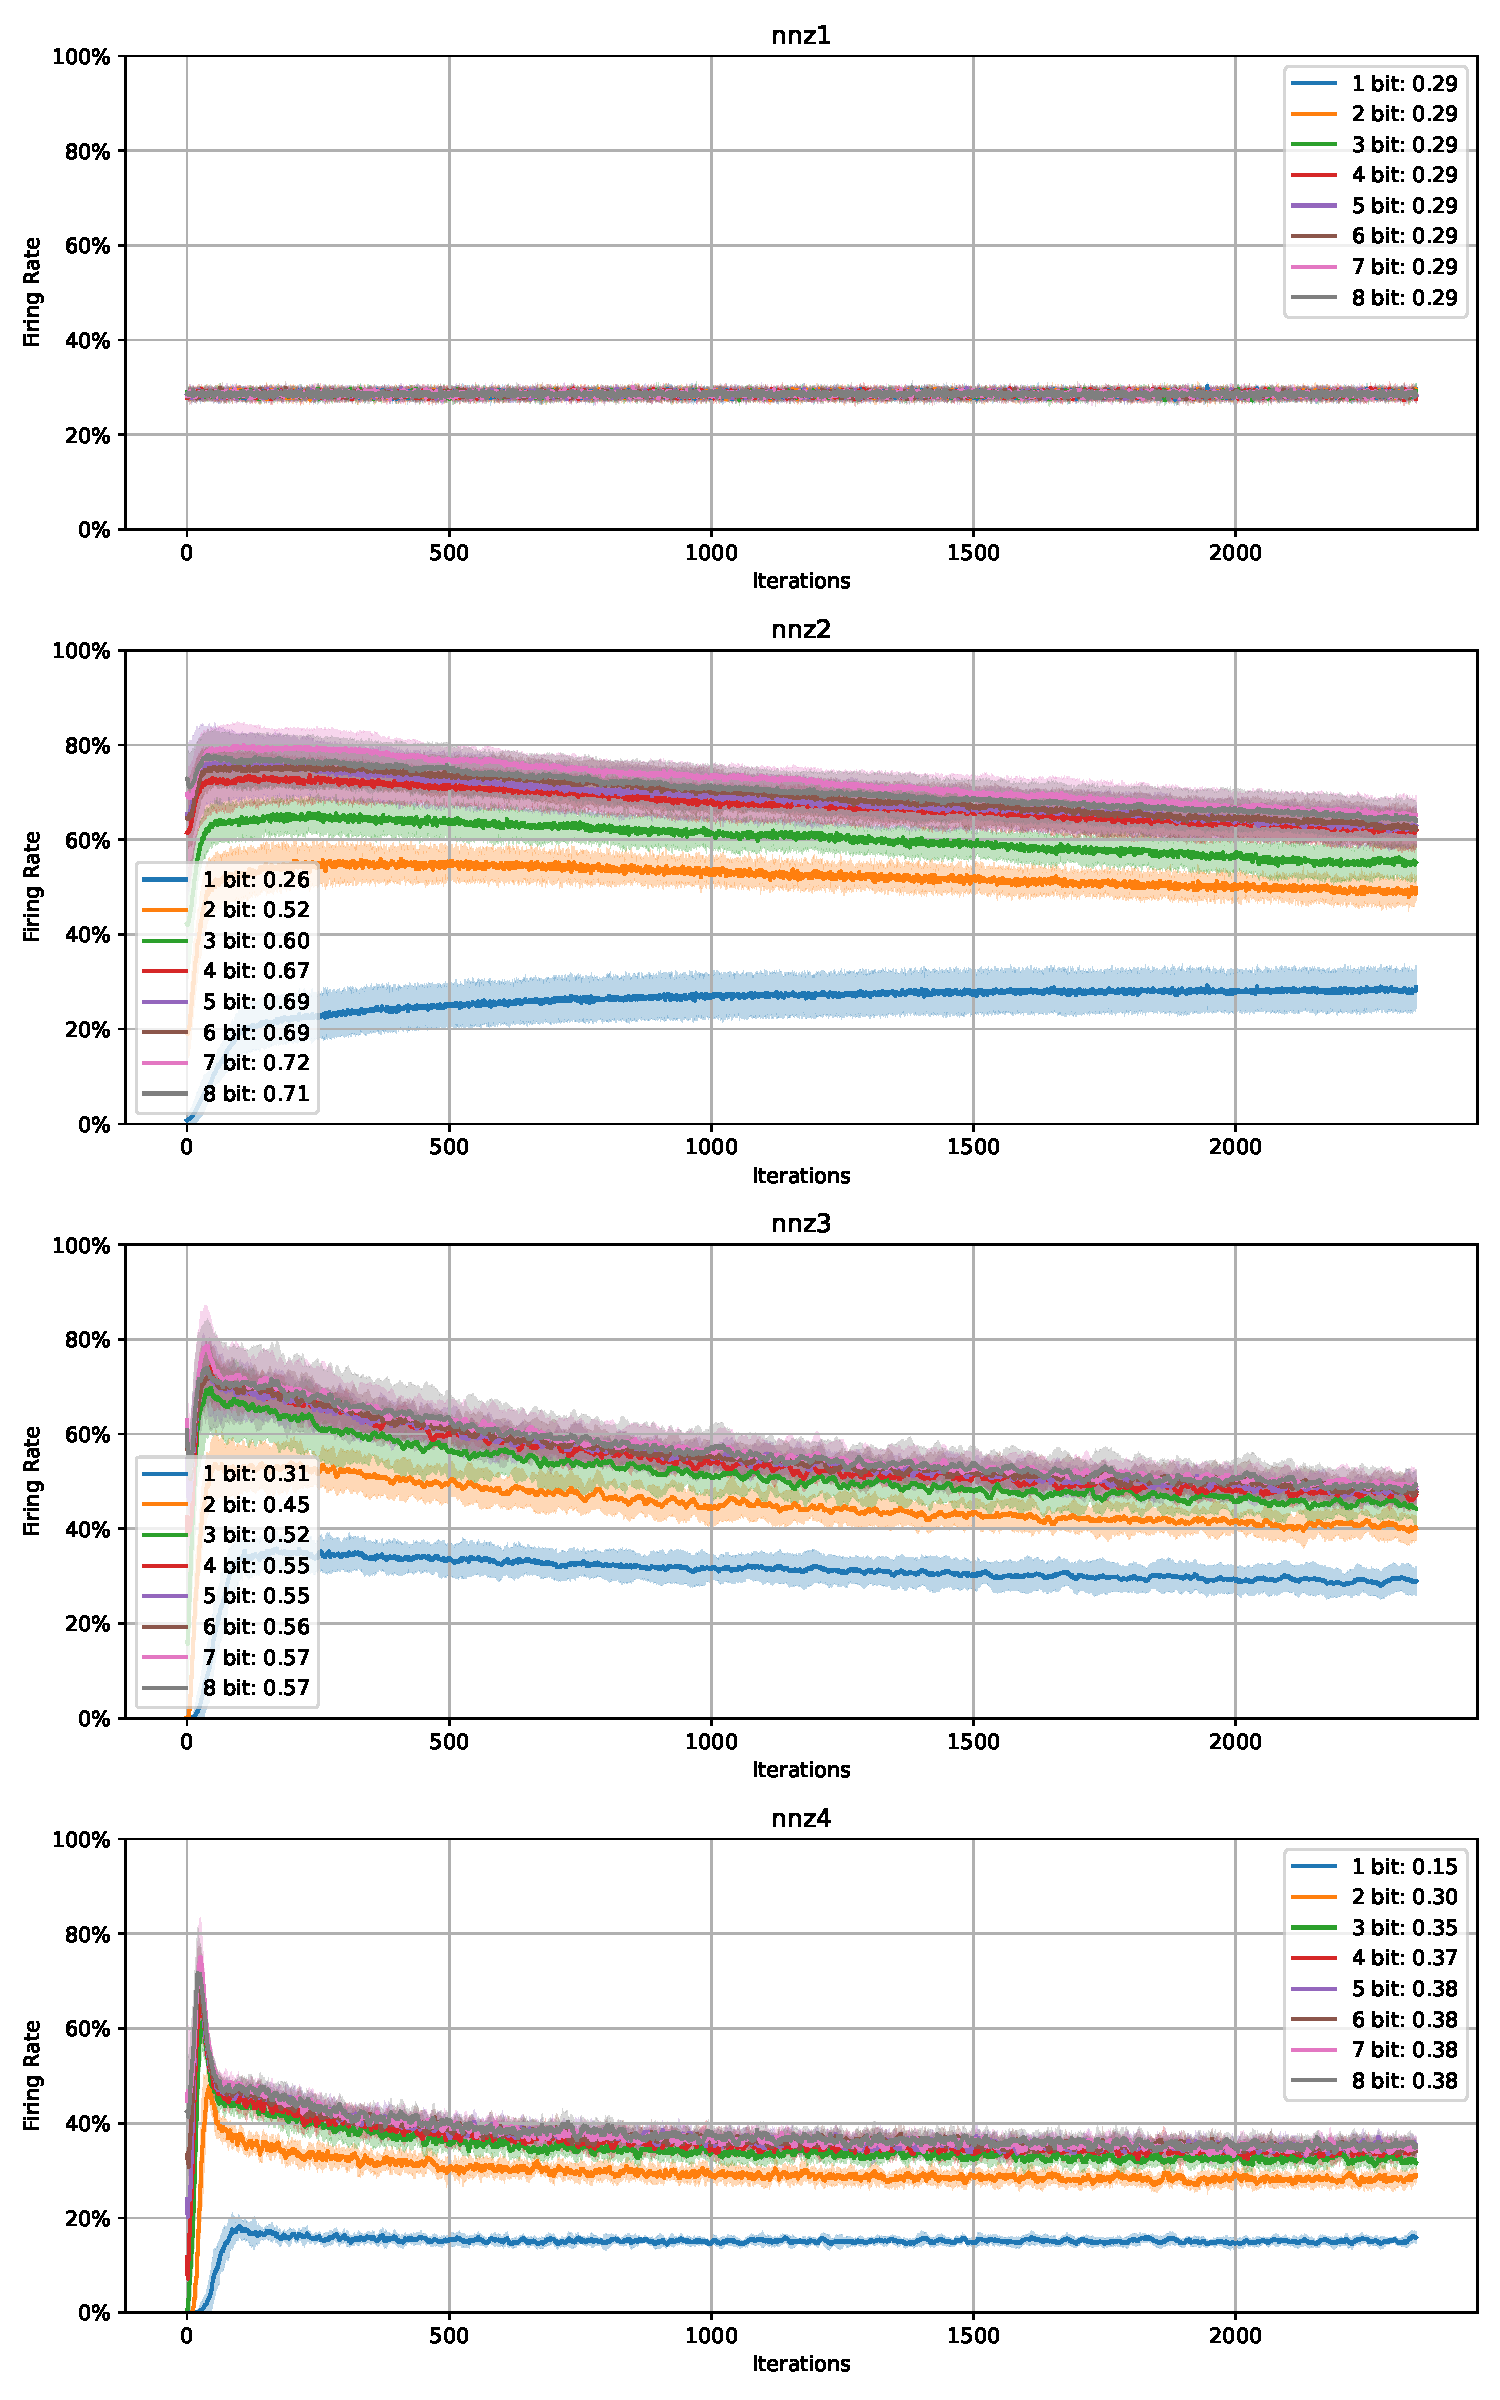
\includegraphics[width=\textwidth]{../firerate/FashionMNIST/plots/fashionmnist_train_firerate.pdf}
                \caption{Firing Rate in Different Positions (Training)}
            \end{subfigure}
        \end{figure}
        \begin{figure}[H]
            \centering
            \ContinuedFloat
            \begin{subfigure}[H]{\textwidth}
                \centering
                \includegraphics[width=\textwidth]{../firerate/FashionMNIST/plots/fashionmnist_test_firerate.pdf}
                \caption{Firing Rate in Different Positions (Test)}
            \end{subfigure}
        \end{figure}
        \begin{figure}[H]
            \centering
            \ContinuedFloat
            \begin{subfigure}[H]{\textwidth}
                \centering
                \includegraphics[width=\textwidth]{../firerate/FashionMNIST/plots/fashionmnist_final_firerate.pdf}
                \caption{Firing Rate in Different Positions (Final Test)}
            \end{subfigure}
            \caption{Firing Rate in Different Positions of the Fashion MNIST Model}
        \end{figure}

    \section{MNIST}
    \label{appendix:firerate_mnist}
        \begin{figure}[H]
            \centering
            \begin{subfigure}[H]{\textwidth}
                \centering
                \includegraphics[width=\textwidth]{../firerate/MNIST/plots/mnist_train_firerate.pdf}
                \caption{Firing Rate in Different Positions (Training)}
            \end{subfigure}
        \end{figure}
        \begin{figure}[H]
            \centering
            \ContinuedFloat
            \begin{subfigure}[H]{\textwidth}
                \centering
                \includegraphics[width=\textwidth]{../firerate/MNIST/plots/mnist_test_firerate.pdf}
                \caption{Firing Rate in Different Positions (Test)}
            \end{subfigure}
        \end{figure}
        \begin{figure}[H]
            \centering
            \ContinuedFloat
            \begin{subfigure}[H]{\textwidth}
                \centering
                \includegraphics[width=\textwidth]{../firerate/MNIST/plots/mnist_final_firerate.pdf}
                \caption{Firing Rate in Different Positions (Final Test)}
            \end{subfigure}
            \caption{Firing Rate in Different Positions of the MNIST Model}
        \end{figure}

    \section{NMNIST}
    \label{appendix:firerate_nmnist}
        \begin{figure}[H]
            \centering
            \begin{subfigure}[H]{\textwidth}
                \centering
                \includegraphics[width=\textwidth]{../firerate/NMNIST/plots/nmnist_train_firerate.pdf}
                \caption{Firing Rate in Different Positions (Training)}
            \end{subfigure}
        \end{figure}
        \begin{figure}[H]
            \centering
            \ContinuedFloat
            \begin{subfigure}[H]{\textwidth}
                \centering
                \includegraphics[width=\textwidth]{../firerate/NMNIST/plots/nmnist_test_firerate.pdf}
                \caption{Firing Rate in Different Positions (Test)}
            \end{subfigure}
        \end{figure}
        \begin{figure}[H]
            \centering
            \ContinuedFloat
            \begin{subfigure}[H]{\textwidth}
                \centering
                \includegraphics[width=\textwidth]{../firerate/NMNIST/plots/nmnist_final_firerate.pdf}
                \caption{Firing Rate in Different Positions (Final Test)}
            \end{subfigure}
            \caption{Firing Rate in Different Positions of the NMNIST Model}
        \end{figure}

    \section{DVS Gesture}
    \label{appendix:firerate_dvs_gesture}
        \begin{figure}[H]
            \centering
            \begin{subfigure}[H]{\textwidth}
                \centering
                \includegraphics[width=\textwidth]{../firerate/DVSGesture/plots/dvsgesture_train_firerate.pdf}
                \caption{Firing Rate in Different Positions (Training)}
            \end{subfigure}
        \end{figure}
        \begin{figure}[H]
            \centering
            \ContinuedFloat
            \begin{subfigure}[H]{\textwidth}
                \centering
                \includegraphics[width=\textwidth]{../firerate/DVSGesture/plots/dvsgesture_test_firerate.pdf}
                \caption{Firing Rate in Different Positions (Test)}
            \end{subfigure}
        \end{figure}
        \begin{figure}[H]
            \centering
            \ContinuedFloat
            \begin{subfigure}[H]{\textwidth}
                \centering
                \includegraphics[width=\textwidth]{../firerate/DVSGesture/plots/dvsgesture_final_firerate.pdf}
                \caption{Firing Rate in Different Positions (Final Test)}
            \end{subfigure}
            \caption{Firing Rate in Different Positions of the DVS Gesture Model}
        \end{figure}

    \section{CIFAR-10}
    \label{appendix:firerate_cifar10}
        Here we use learning rate schedulers to accelerate the convergence of the models. Although the models can reach a high accuracy faster, the multi-bit spike train model suffers from the high learning rate from time to time. 

        \begin{figure}[H]
            \centering
            \begin{subfigure}[H]{\textwidth}
                \centering
                \includegraphics[width=\textwidth]{../firerate/CIFAR10/plots/cifar10_train_firerate.pdf}
                \caption{Firing Rate in Different Positions (Training)}
            \end{subfigure}
        \end{figure}
        \begin{figure}[H]
            \centering
            \ContinuedFloat
            \begin{subfigure}[H]{\textwidth}
                \centering
                \includegraphics[width=\textwidth]{../firerate/CIFAR10/plots/cifar10_test_firerate.pdf}
                \caption{Firing Rate in Different Positions (Test)}
            \end{subfigure}
        \end{figure}
        \begin{figure}[H]
            \centering
            \ContinuedFloat
            \begin{subfigure}[H]{\textwidth}
                \centering
                \includegraphics[width=\textwidth]{../firerate/CIFAR10/plots/cifar10_final_firerate.pdf}
                \caption{Firing Rate in Different Positions (Final Test)}
            \end{subfigure}
            \caption{Firing Rate in Different Positions of the CIFAR-10 Model}
        \end{figure}

\chapter{Energy Consumption Estimation}
\label{appendix:energy}

\section{Training Energy Consumption Estimation on GPUs}
\label{appendix:energy_gpu}

    The hyperparameters used in the training process are the same as in Table \ref{tab:hyperparameters_accuracy}.

    \label{appendix:energy_gpu_fashion_mnist}

        \begin{figure}[H]
            \centering
            \begin{subfigure}[H]{\textwidth}
                \includegraphics[width=\textwidth]{../standard/FashionMNIST/plots/fashionmnist_train_energy_gpu_horizontal.pdf}
                \caption{Energy Consumption Estimation, Unit in Constant $c$}
            \end{subfigure}
        \end{figure}
        \begin{figure}[H]
            \centering
            \ContinuedFloat
            \begin{subfigure}[H]{\textwidth}
                \includegraphics[width=\textwidth]{../standard/FashionMNIST/plots/fashionmnist_train_relative_energy_gpu_horizontal.pdf}
                \caption{Normalized Energy Consumption Estimation Relative to 1-bit Spike Train Model}
            \end{subfigure}
            \caption{Training Energy Consumption Estimation on GPUs for Fashion MNIST Dataset}
        \end{figure}

    \label{appendix:energy_gpu_mnist}

        \begin{figure}[H]
            \centering
            \begin{subfigure}[H]{\textwidth}
                \includegraphics[width=\textwidth]{../standard/MNIST/plots/mnist_train_energy_gpu_horizontal.pdf}
                \caption{Energy Consumption Estimation, Unit in Constant $c$}
            \end{subfigure}
        \end{figure}
        \begin{figure}[H]
            \centering
            \ContinuedFloat
            \begin{subfigure}[H]{\textwidth}
                \includegraphics[width=\textwidth]{../standard/MNIST/plots/mnist_train_relative_energy_gpu_horizontal.pdf}
                \caption{Normalized Energy Consumption Estimation Relative to 1-bit Spike Train Model}
            \end{subfigure}
            \caption{Training Energy Consumption Estimation on GPUs for MNIST Dataset}
        \end{figure}

    \label{appendix:energy_gpu_nmnist}

        \begin{figure}[H]
            \centering
            \begin{subfigure}[H]{\textwidth}
                \includegraphics[width=\textwidth]{../standard/NMNIST/plots/nmnist_train_energy_gpu_horizontal.pdf}
                \caption{Energy Consumption Estimation, Unit in Constant $c$}
            \end{subfigure}
        \end{figure}
        \begin{figure}[H]
            \centering
            \ContinuedFloat
            \begin{subfigure}[H]{\textwidth}
                \includegraphics[width=\textwidth]{../standard/NMNIST/plots/nmnist_train_relative_energy_gpu_horizontal.pdf}
                \caption{Normalized Energy Consumption Estimation Relative to 1-bit Spike Train Model}
            \end{subfigure}
            \caption{Training Energy Consumption Estimation on GPUs for NMNIST Dataset}
        \end{figure}

    \label{appendix:energy_gpu_dvs_gesture}

        \begin{figure}[H]
            \centering
            \begin{subfigure}[H]{\textwidth}
                \includegraphics[width=\textwidth]{../standard/DVSGesture/plots/dvsgesture_train_energy_gpu_horizontal.pdf}
                \caption{Energy Consumption Estimation, Unit in Constant $c$}
            \end{subfigure}
        \end{figure}
        \begin{figure}[H]
            \centering
            \ContinuedFloat
            \begin{subfigure}[H]{\textwidth}
                \includegraphics[width=\textwidth]{../standard/DVSGesture/plots/dvsgesture_train_relative_energy_gpu_horizontal.pdf}
                \caption{Normalized Energy Consumption Estimation Relative to 1-bit Spike Train Model}
            \end{subfigure}
            \caption{Training Energy Consumption Estimation on GPUs for DVS Gesture Dataset}
        \end{figure}

    \label{appendix:energy_gpu_cifar10}

        \begin{figure}[H]
            \centering
            \begin{subfigure}[H]{\textwidth}
                \includegraphics[width=\textwidth]{../standard/CIFAR10/plots/cifar10_train_energy_gpu_horizontal.pdf}
                \caption{Energy Consumption Estimation, Unit in Constant $c$}
            \end{subfigure}
        \end{figure}
        \begin{figure}[H]
            \centering
            \ContinuedFloat
            \begin{subfigure}[H]{\textwidth}
                \includegraphics[width=\textwidth]{../standard/CIFAR10/plots/cifar10_train_relative_energy_gpu_horizontal.pdf}
                \caption{Normalized Energy Consumption Estimation Relative to 1-bit Spike Train Model}
            \end{subfigure}
            \caption{Training Energy Consumption Estimation on GPUs for CIFAR-10 Dataset}
        \end{figure}

\section{Inference Energy Consumption Estimation on Neuromorphic Hardware}
\label{appendix:energy_neuromorphic}

    We assume the models are running on neuromorphic hardware like Intel Loihi 2 that support graded spikes. 

    The hyperparameters used in the training process are the same as in Table \ref{tab:hyperparameters_accuracy}.

    \subsection{Fashion MNIST}
    \label{appendix:energy_neuromorphic_fashion_mnist}

        % \begin{figure}[H]
        %     \centering
        %     \begin{subfigure}[H]{0.495\textwidth}
        %         \includegraphics[width=\textwidth]{../standard/FashionMNIST/plots/fashionmnist_test_energy_nh.pdf}
        %         \caption{Energy Consumption Estimation, Unit in Parameters $F\cdot E_{\text{AC}}$}
        %     \end{subfigure}
        %     \hfill
        %     \begin{subfigure}[H]{0.495\textwidth}
        %         \includegraphics[width=\textwidth]{../standard/FashionMNIST/plots/fashionmnist_test_relative_energy_nh.pdf}
        %         \caption{Normalized Energy Consumption Estimation Relative to 1-bit Spike Train Model}
        %     \end{subfigure}
        %     \caption{Inference Energy Consumption Estimation on Intel Loihi 2}
        % \end{figure}
        \begin{figure}[H]
            \centering
            \begin{subfigure}[H]{0.7\textwidth}
                \centering
                \includegraphics[width=\textwidth]{../standard/FashionMNIST/plots/fashionmnist_test_energy_nh.pdf}
                \caption{Energy Consumption Estimation, Unit in Parameters $F\cdot E_{\text{AC}}$}
            \end{subfigure}
        \end{figure}
        \begin{figure}[H]
            \centering
            \ContinuedFloat
            \begin{subfigure}[H]{0.7\textwidth}
                \centering
                \includegraphics[width=\textwidth]{../standard/FashionMNIST/plots/fashionmnist_test_relative_energy_nh.pdf}
                \caption{Normalized Energy Consumption Estimation Relative to 1-bit Spike Train Model}
            \end{subfigure}
            \caption{Inference Energy Consumption Estimation on Intel Loihi 2}
        \end{figure}
    
    \subsection{MNIST}
    \label{appendix:energy_neuromorphic_mnist}

        % \begin{figure}[H]
        %     \centering
        %     \begin{subfigure}[H]{0.495\textwidth}
        %         \includegraphics[width=\textwidth]{../standard/MNIST/plots/mnist_test_energy_nh.pdf}
        %         \caption{Energy Consumption Estimation, Unit in Parameters $F\cdot E_{\text{AC}}$}
        %     \end{subfigure}
        %     \hfill
        %     \begin{subfigure}[H]{0.495\textwidth}
        %         \includegraphics[width=\textwidth]{../standard/MNIST/plots/mnist_test_relative_energy_nh.pdf}
        %         \caption{Normalized Energy Consumption Estimation Relative to 1-bit Spike Train Model}
        %     \end{subfigure}
        %     \caption{Inference Energy Consumption Estimation on Intel Loihi 2}
        % \end{figure}
        \begin{figure}[H]
            \centering
            \begin{subfigure}[H]{0.7\textwidth}
                \centering
                \includegraphics[width=\textwidth]{../standard/MNIST/plots/mnist_test_energy_nh.pdf}
                \caption{Energy Consumption Estimation, Unit in Parameters $F\cdot E_{\text{AC}}$}
            \end{subfigure}
        \end{figure}
        \begin{figure}[H]
            \centering
            \ContinuedFloat
            \begin{subfigure}[H]{0.7\textwidth}
                \centering
                \includegraphics[width=\textwidth]{../standard/MNIST/plots/mnist_test_relative_energy_nh.pdf}
                \caption{Normalized Energy Consumption Estimation Relative to 1-bit Spike Train Model}
            \end{subfigure}
            \caption{Inference Energy Consumption Estimation on Intel Loihi 2}
        \end{figure}

    \subsection{NMNIST}
    \label{appendix:energy_neuromorphic_nmnist}

        % \begin{figure}[H]
        %     \centering
        %     \begin{subfigure}[H]{0.495\textwidth}
        %         \includegraphics[width=\textwidth]{../standard/NMNIST/plots/nmnist_test_energy_nh.pdf}
        %         \caption{Energy Consumption Estimation, Unit in Parameters $F\cdot E_{\text{AC}}$}
        %     \end{subfigure}
        %     \hfill
        %     \begin{subfigure}[H]{0.495\textwidth}
        %         \includegraphics[width=\textwidth]{../standard/NMNIST/plots/nmnist_test_relative_energy_nh.pdf}
        %         \caption{Normalized Energy Consumption Estimation Relative to 1-bit Spike Train Model}
        %     \end{subfigure}
        %     \caption{Inference Energy Consumption Estimation on Intel Loihi 2}
        % \end{figure}
        \begin{figure}[H]
            \centering
            \begin{subfigure}[H]{0.7\textwidth}
                \centering
                \includegraphics[width=\textwidth]{../standard/NMNIST/plots/nmnist_test_energy_nh.pdf}
                \caption{Energy Consumption Estimation, Unit in Parameters $F\cdot E_{\text{AC}}$}
            \end{subfigure}
        \end{figure}
        \begin{figure}[H]
            \centering
            \ContinuedFloat
            \begin{subfigure}[H]{0.7\textwidth}
                \centering
                \includegraphics[width=\textwidth]{../standard/NMNIST/plots/nmnist_test_relative_energy_nh.pdf}
                \caption{Normalized Energy Consumption Estimation Relative to 1-bit Spike Train Model}
            \end{subfigure}
            \caption{Inference Energy Consumption Estimation on Intel Loihi 2}
        \end{figure}

    \subsection{DVS Gesture}
    \label{appendix:energy_neuromorphic_dvs_gesture}

        % \begin{figure}[H]
        %     \centering
        %     \begin{subfigure}[H]{0.495\textwidth}
        %         \includegraphics[width=\textwidth]{../standard/DVSGesture/plots/dvsgesture_test_energy_nh.pdf}
        %         \caption{Energy Consumption Estimation, Unit in Parameters $F\cdot E_{\text{AC}}$}
        %     \end{subfigure}
        %     \hfill
        %     \begin{subfigure}[H]{0.495\textwidth}
        %         \includegraphics[width=\textwidth]{../standard/DVSGesture/plots/dvsgesture_test_relative_energy_nh.pdf}
        %         \caption{Normalized Energy Consumption Estimation Relative to 1-bit Spike Train Model}
        %     \end{subfigure}
        %     \caption{Inference Energy Consumption Estimation on Intel Loihi 2}
        % \end{figure}
        \begin{figure}[H]
            \centering
            \begin{subfigure}[H]{0.7\textwidth}
                \centering
                \includegraphics[width=\textwidth]{../standard/DVSGesture/plots/dvsgesture_test_energy_nh.pdf}
                \caption{Energy Consumption Estimation, Unit in Parameters $F\cdot E_{\text{AC}}$}
            \end{subfigure}
        \end{figure}
        \begin{figure}[H]
            \centering
            \ContinuedFloat
            \begin{subfigure}[H]{0.7\textwidth}
                \centering
                \includegraphics[width=\textwidth]{../standard/DVSGesture/plots/dvsgesture_test_relative_energy_nh.pdf}
                \caption{Normalized Energy Consumption Estimation Relative to 1-bit Spike Train Model}
            \end{subfigure}
            \caption{Inference Energy Consumption Estimation on Intel Loihi 2}
        \end{figure}

    \subsection{CIFAR-10}
    \label{appendix:energy_neuromorphic_cifar10}

        % \begin{figure}[H]
        %     \centering
        %     \begin{subfigure}[H]{0.495\textwidth}
        %         \includegraphics[width=\textwidth]{../standard/CIFAR10/plots/cifar10_test_energy_nh.pdf}
        %         \caption{Energy Consumption Estimation, Unit in Parameters $F\cdot E_{\text{AC}}$}
        %     \end{subfigure}
        %     \hfill
        %     \begin{subfigure}[H]{0.495\textwidth}
        %         \includegraphics[width=\textwidth]{../standard/CIFAR10/plots/cifar10_test_relative_energy_nh.pdf}
        %         \caption{Normalized Energy Consumption Estimation Relative to 1-bit Spike Train Model}
        %     \end{subfigure}
        %     \caption{Inference Energy Consumption Estimation on Intel Loihi 2}
        % \end{figure}
        \begin{figure}[H]
            \centering
            \begin{subfigure}[H]{0.7\textwidth}
                \centering
                \includegraphics[width=\textwidth]{../standard/CIFAR10/plots/cifar10_test_energy_nh.pdf}
                \caption{Energy Consumption Estimation, Unit in Parameters $F\cdot E_{\text{AC}}$}
            \end{subfigure}
        \end{figure}
        \begin{figure}[H]
            \centering
            \ContinuedFloat
            \begin{subfigure}[H]{0.7\textwidth}
                \centering
                \includegraphics[width=\textwidth]{../standard/CIFAR10/plots/cifar10_test_relative_energy_nh.pdf}
                \caption{Normalized Energy Consumption Estimation Relative to 1-bit Spike Train Model}
            \end{subfigure}
            \caption{Inference Energy Consumption Estimation on Intel Loihi 2}
        \end{figure}

\section{Trading Accuracy for Energy Consumption}
\label{appendix:energy_tradeoff}

    The hyperparameters used in the training process are shown in Table \ref{tab:hyperparameters_energy_tradeoff}.

    \begin{table}[H]
        \begin{tabularx}{\textwidth}{|X|c|c|c|c|c|c|c|}
            \toprule
            Dataset & Reps & Epochs & LR & Opt & Batch & Time steps \\
            \midrule
            Fashion MNIST & 10 & 5 & 2e-3 & Adam & 128 & 4 \\
            CIFAR-10 & 5 & 50 & 1e-5 & Adam & 128 & 4 \\
            \bottomrule
        \end{tabularx}
        \caption{Hyperparameters}
        \label{tab:hyperparameters_energy_tradeoff}
    \end{table}

    \subsection{Fashion MNIST}
    \label{appendix:energy_tradeoff_fashion_mnist}

        \begin{figure}[H]
            \centering
            \begin{subfigure}[H]{\textwidth}
                \centering
                \begin{subfigure}[H]{\textwidth}
                    \includegraphics[width=\textwidth]{../timesteps/FashionMNIST/plots/fashionmnist_train_acc.pdf}
                    \caption{Training Accuracy (smoothed with a window size of 100)}
                \end{subfigure}
                \hfill
                \begin{subfigure}[H]{\textwidth}
                    \includegraphics[width=\textwidth]{../timesteps/FashionMNIST/plots/fashionmnist_test_acc.pdf}
                    \caption{Test Accuracy}
                \end{subfigure}
            \end{subfigure}
            \hfill
            \begin{subfigure}[H]{\textwidth}
                \centering
                \includegraphics[width=0.8\textwidth]{../timesteps/FashionMNIST/plots/fashionmnist_final_acc_horizontal.pdf}
                \caption{Final Test Accuracy}
            \end{subfigure}
            \caption{Accuracy of 1-bit Spike Train Model with 10 Timesteps and 2-bit Spike Train Model with 4 Timesteps}
        \end{figure}

        \begin{figure}[H]
            \centering
            \begin{subfigure}[H]{\textwidth}
                \includegraphics[width=\textwidth]{../timesteps/FashionMNIST/plots/fashionmnist_train_energy_gpu_horizontal.pdf}
                \caption{Energy Consumption Estimation, Unit in Constant $c$}
            \end{subfigure}
            \hfill
            \begin{subfigure}[H]{\textwidth}
                \includegraphics[width=\textwidth]{../timesteps/FashionMNIST/plots/fashionmnist_train_relative_energy_gpu_horizontal.pdf}
                \caption{Normalized Energy Consumption Estimation Relative to 1-bit Spike Train Model}
            \end{subfigure}
            \caption{Training Energy Consumption Estimation on GPUs for Fashion MNIST Dataset}
        \end{figure}

        \begin{figure}[H]
            \centering
            \begin{subfigure}[H]{0.495\textwidth}
                \includegraphics[width=\textwidth]{../timesteps/FashionMNIST/plots/fashionmnist_test_energy_nh.pdf}
                \caption{Energy Consumption Estimation, Unit in Parameters $F\cdot E_{\text{AC}}$}
            \end{subfigure}
            \hfill
            \begin{subfigure}[H]{0.495\textwidth}
                \includegraphics[width=\textwidth]{../timesteps/FashionMNIST/plots/fashionmnist_test_relative_energy_nh.pdf}
                \caption{Normalized Energy Consumption Estimation Relative to 1-bit Spike Train Model}
            \end{subfigure}
            \caption{Inference Energy Consumption Estimation on Intel Loihi 2}
        \end{figure}

    \subsection{CIFAR-10}
    \label{appendix:energy_tradeoff_cifar10}

        \begin{figure}[H]
            \centering
            \begin{subfigure}[H]{\textwidth}
                \centering
                \begin{subfigure}[H]{\textwidth}
                    \includegraphics[width=\textwidth]{../timesteps/CIFAR10/plots/cifar10_train_acc.pdf}
                    \caption{Training Accuracy (smoothed with a window size of 100)}
                \end{subfigure}
                \hfill
                \begin{subfigure}[H]{\textwidth}
                    \includegraphics[width=\textwidth]{../timesteps/CIFAR10/plots/cifar10_test_acc.pdf}
                    \caption{Test Accuracy}
                \end{subfigure}
            \end{subfigure}
            \hfill
            \begin{subfigure}[H]{0.8\textwidth}
                \centering
                \includegraphics[width=\textwidth]{../timesteps/CIFAR10/plots/cifar10_final_acc_horizontal.pdf}
                \caption{Final Test Accuracy}
            \end{subfigure}
            \caption{Accuracy of 1-bit Spike Train Model with 10 Timesteps and 2-bit Spike Train Model with 4 Timesteps}
        \end{figure}

        \begin{figure}[H]
            \centering
            \begin{subfigure}[H]{\textwidth}
                \includegraphics[width=\textwidth]{../timesteps/CIFAR10/plots/cifar10_train_energy_gpu_horizontal.pdf}
                \caption{Energy Consumption Estimation, Unit in Constant $c$}
            \end{subfigure}
            \hfill
            \begin{subfigure}[H]{\textwidth}
                \includegraphics[width=\textwidth]{../timesteps/CIFAR10/plots/cifar10_train_relative_energy_gpu_horizontal.pdf}
                \caption{Normalized Energy Consumption Estimation Relative to 1-bit Spike Train Model}
            \end{subfigure}
            \caption{Training Energy Consumption Estimation on GPUs for CIFAR-10 Dataset}
        \end{figure}

        \begin{figure}[H]
            \centering
            \begin{subfigure}[H]{0.495\textwidth}
                \includegraphics[width=\textwidth]{../timesteps/CIFAR10/plots/cifar10_test_energy_nh.pdf}
                \caption{Energy Consumption Estimation, Unit in Parameters $F\cdot E_{\text{AC}}$}
            \end{subfigure}
            \hfill
            \begin{subfigure}[H]{0.495\textwidth}
                \includegraphics[width=\textwidth]{../timesteps/CIFAR10/plots/cifar10_test_relative_energy_nh.pdf}
                \caption{Normalized Energy Consumption Estimation Relative to 1-bit Spike Train Model}
            \end{subfigure}
            \caption{Inference Energy Consumption Estimation on Intel Loihi 2}
        \end{figure}


\backmatter

\bibliographystyle{plain}
\bibliography{refs}

\includepdf[pages={-}]{declaration-originality.pdf}

\end{document}
